\documentclass[12pt,twoside]{report}
\usepackage[utf8]{inputenc}
%Para qué los títulos aparezcan en español
\usepackage[spanish]{babel}
\usepackage{csquotes}
\usepackage{array} % para hacer tablas
\usepackage{graphicx} % gráficos
\usepackage{booktabs} %para que las tablas se vean como en los libros y revistas
\usepackage{float} % posiciona las imágenes, tambien usamos placeins
\usepackage{blindtext}
\usepackage{caption} %para los subtítulos de cuadros y figuras
\usepackage{placeins} %para el posicionamiento de imágenes
\usepackage{subfig}
\usepackage[export]{adjustbox}
\usepackage{verbatim} % comentarios
\raggedbottom  %para eliminar los espacios en blanco que deja el espaciado automatico.
%\usepackage{amssymb}
\usepackage[
backend=biber,
sorting=none
]{biblatex} %se puede especificar otra forma de imprimir las citaciones aca
\addbibresource{referencias.bib}

%Margenes según normas APA
\usepackage[a4paper,top=1in, bottom=1in, left=1in, right=1in]{geometry}

% Links a todo el documento y urls
\usepackage{hyperref}
\hypersetup{
    colorlinks=true,
    linkcolor=blue,
    filecolor=magenta,      
    urlcolor=black,
    citecolor=black,
    pdftitle={Sharelatex Example},
    %bookmarks=true,
    pdfpagemode=FullScreen,
}

\begin{document}

    \begin{titlepage}

    \begin{center}

        \begin{tabular}{ p{0.5\textwidth} p{0.5\textwidth} }
        		\centering
\includegraphics[height=0.15\textwidth]{./imagenes_caratula/unc_logo.jpg} &
        		\centering
\includegraphics[height=0.15\textwidth]{./imagenes_caratula/logo_fcefyn_nuevo.jpg}
        \end{tabular}
        
        \vspace*{30mm}
        \begin{Huge}
            Universidad Nacional de Córdoba \\
        \end{Huge}
        
        \vspace*{10mm}
        \begin{Large}
            Facultad de Ciencias Exactas Físicas y Naturales \\
        \end{Large}
        
        \vspace*{20mm}
        \begin{large}
            Proyecto Integrador: \\
        \end{large}
        
        \vspace*{5mm}
        \begin{LARGE}
            \textbf{Implementación de una solución para gestión de eventos de seguridad de una red de datos} \\
        \end{LARGE}
        
        \vspace*{0.3in}
        \begin{large} \begin{center}
          Autores  
        \end{center}
        \end{large}
        \begin{center}
           \begin{table}[h]
            \resizebox{\textwidth}{!}{%
            \begin{tabular}{|rll|}
            \hline
            \multicolumn{1}{|l}{} & Figueroa Sergio David        & Sepulveda Federico Nicolas       \\
            Correo:               & sergiofigueroa@mi.unc.edu.ar & federico.sepulveda@mi.unc.edu.ar \\
            Matricula:            & 36355236                     & 35037929                         \\
            Telefono:             & 3512941114               & 2994165771                   \\ \hline
            \end{tabular}%
            }
            \end{table}
        \end{center}
        \vspace*{0.3mm}
        \rule{100mm}{0.1mm}\\
        \vspace*{0.3mm}
        \begin{large}
            Director: \\
            Mgter. Ing. Miguel Ángel Solinas \\
        \end{large}
        

    \end{center}

\end{titlepage}

    \chapter*{\Large Resumen}
\addcontentsline{toc}{chapter}{Resumen}


    % Índice general
    \tableofcontents
    % Índice de figuras
    \listoffigures
    % Índice de tablas
    \listoftables
    % Agradecimientos
    \chapter*{\Large Agradecimientos}
\addcontentsline{toc}{chapter}{Agradecimientos}

A toda mi gran Familia por su apoyo permanente: mi abuela Yoli, mis padres, mis hermanos, mis abuelos Sergio, Cesar y mi Nona, tíos y primos. Mi novia Victoria, mis amigos Alan y Antonio que me ayudaron en el trabajo mientras necesitaba concentrarme en esta tesis y a todos los amigos y compañeros de la facultad, junto a los que recorrí este desafiante y apasionante camino que es la carrera de Ingeniería en Computación. Sin ellos, sin lugar a dudas todo hubiera sido mas difícil. \par Mi ultimo agradecimiento es hacia la Universidad Nacional de Córdoba y la Facultad de Ciencias Exactas, Físicas y Naturales, por la educación gratuita y de calidad que recibí para mi formación.\par 
\begin{large} \begin{center}
         Sergio David Figueroa 
        \end{center}
        \end{large}

Agradezco a mi familia que me apoyo durante toda la carrera. También a mis amigos y compañeros que hicieron que transitar por la facultad fuera una experiencia mas llevadera. Y agradezco que exista la Universidad publica y gratuita. \par
\begin{large} \begin{center}
         Federico Nicolas Sepulveda 
        \end{center}
        \end{large}
    % Glosario
    \chapter*{\Large Glosario}
\addcontentsline{toc}{chapter}{Glosario}

\textbf{CCNA}: siglas en inglés de Cisco Certified Network Associate, un certificado de validación profesional emitido por la corporación Cisco para técnicos que operan sus productos. \par

\textbf{CERT}: siglas en inglés de Computer Emergency Response Team, en español equipo de respuesta a incidentes de computadoras. Término registrado comercialmente por la universidad estadounidense de Carnegie Mellon. \par

\textbf{CPU}: siglas en inglés de Central Processing Unit, en español Unidad de Procesamiento Central.\par

\textbf{Creative Commons}: licencia que permite a cualquier usuario copiar, reproducir, adaptar, distribuir, traducir y desarrollar los contenidos multimedia sin costo alguno. La utilización de contenido que se encuentra bajo esta licencia implica reconocer al autor original.\par

\textbf{CSIRT}: siglas en inglés de Computer Security Incident Response Team, en español equipo de respuesta a incidentes de seguridad de computación. Es el equipo de profesionales, sistemas y toda la infraestructura (hardware y software) de detección y respuesta a incidentes de ciberseguridad de una organización.\par

\textbf{DDoS}: siglas en inglés de Denied Distribution Of Service, en español denegación distribuida de servicio. \par

\textbf{DNS}: siglas en inglés de Domain Name Service, en español Servicio de Nombres de Dominio, es un protocolo de red de la capa de aplicación. \par


\textbf{Dirección MAC}: siglas en inglés de Media Access Control, en español control de acceso a medios, es un conjunto de bytes que constituyen la dirección física (única) que identifica a un dispositivo conectado a una red. \par

\textbf{EMCFFAA}: siglas del Estado Mayor Conjunto de las Fuerzas Armadas Argentinas. \par

\textbf{Firewall}: Un firewall es un dispositivo basado en un software, hardware o ambos. Bloquea o permite el tráfico de red, basándose en una serie de reglas dinámicas predefinidas y políticas. \par

\textbf{Gbps}: siglas de gigabit por segundo, es una especificación técnica de la medida del ancho de banda y / o velocidad de transmisión, dependiendo del contexto. \par

\textbf{GNU}: acrónimo recursivo en inglés de “GNU is Not Unix”, en español "GNU No es Unix". \par

\textbf{GPL}: siglas en inglés de General Public Licence, en español licencia pública general, es un tipo de licencia GNU. \par

\textbf{GUI}: siglas en inglés de Graphical User Interface, en español Interfaz gráfica de Usuario. \par

\textbf{HIDS}: siglas en inglés de Host Intrusion Detection System, en español sistema de detección de intrusiones en un host o punto final. \par

\textbf{IDS}: siglas en inglés de Intrusion Detection System, en español sistema de detección de intrusiones. Es un componente de software destinado al procesamiento de firmas basadas en la información recolectada del tráfico de red, mediante una sonda colocada en un enlace de la infraestructura de comunicaciones de datos. Los IDS son un componente vital de un CSIRT debido a que realizan la identificación a priori de eventos en el tráfico de datos y su clasificación como un incidente. \par

\textbf{IMAP}:  siglas en inglés de Internet Message Access Protocol. Este protocolo de aplicación, permite a los usuarios acceder a sus e-mails directamente en el servidor y sólo descargar, hacia la máquina local, los mensajes y archivos adjuntos que le resulten de interés. \par

\textbf{Información normalizada}: el objetivo es modificar los mensajes de diferentes fuentes de manera tal que se adapten a un modelo de datos común. \par

\textbf{Infraestructura de IT}: corresponde a la infraestructura de tecnologías de la información (servidores, switches, routers, etc) de una organización. \par

\textbf{IPV4 e IVP6}: siglas en inglés de los protocolos de Internet versiones 4 y 6, respectivamente. \par

\textbf{IPS}: siglas en inglés de Intrusion Protection System, en español sistema de protección de intrusiones. \par

\textbf{Licencia AGPL}: siglas de GNU Affero General Public License. Esta licencia asegura los derechos de autor sobre el software y da permisos legales para la copia, distribución y modificaciones del mismo. En caso de modificaciones se debe poner a disposición de la comunidad el código fuente con dichos cambios. \par

\textbf{Licencia APACHE}: licencia de software libre permisiva creada por la Apache Software Foundation. Se diferencia de otros tipos de licencias ya que no exige copyleft en el software donde se aplica. \par

\textbf{Licencia BSD}: siglas en inglés de Berkeley Software Distribution, licencia de software libre desarrollada en dicha universidad homónima de Estados Unidos. \par

\textbf{Licencia GFDL}: siglas de GNU Free Documentation License. Está orientado a permitir que un manual, un libro de texto o cualquier  otro documento escrito sea libre en el sentido de su difusión, copias, modificaciones y comercialización. \par

\textbf{Linux}: núcleo de código (kernel) abierto de familias de sistemas operativos del mismo nombre, de software libre. \par

\textbf{Log}: equivalente en inglés a “registro” en español. Término utilizado específicamente para registros de datos con un formato definido. \par

\textbf{Malware}: software malicioso diseñado para identificar y / o explotar vulnerabilidades en  los sistemas de  una víctima: sistemas operativos, drivers, cualquier tipo de software, dispositivos, etc. Las consecuencias implican desde el mal funcionamiento del software o dispositivo afectado, robo o pérdida de información, hasta la inutilización total del hardware o sistema infectado. \par

\textbf{MIT}: siglas en inglés de Massachusetts Institute of Technology, universidad de los Estados Unidos cuyo nombre es usado para un tipo de licencia de código libre desarrollada en esa universidad. \par
\textbf{MSSP}: siglas 
en inglés de Managed Security Service Provider", en español proveedores de servicios de seguridad gestionados. Empresas que prestan servicios de seguridad informática a organizaciones. \par

\textbf{NIDS}: siglas en inglés de Network Intrusion Detection System, en español sistema de detección de intrusiones a nivel de red. \par

\textbf{NIPS}: siglas en inglés de Network Intrusion Protection System, en español sistema de protección de intrusiones a nivel de red. \par

\textbf{NSM}: siglas en inglés de Network Security Monitoring, en español monitoreo de seguridad de redes. \par

\textbf{RAM}: siglas en inglés de Random Access Memory, en español memoria de acceso aleatorio. \par

\textbf{Ransomware}: Software malicioso, que en un dispositivo puede bloquear la interfaz de usuario o cifrar las información que se encuentra en el disco y posteriormente solicitarle a la víctima un pago para recuperar los datos. \par

\textbf{SaaS}: siglas en inglés de Software as a Service, en español software como servicio, es un modelo de negocio de software, cuyo despliegue y funcionalidades están disponibles a la medida de la demanda del cliente. \par

\textbf{SNMP}: Simple Network Management Protocol (Protocolo simple de administración de red, por sus siglas en ingles). Protocolo que se ubica en el nivel de aplicación de la pila de red TCP/IP.  \par

\textbf{STDIN}: siglas en ingles de Standard Input, es la entrada estándar de ingreso de datos a un software.\par

\textbf{SYN}: bit usado en el protocolo TCP para indicar la sincronización del número de secuencia al comienzo de una comunicación utilizando el protocolo antes mencionado. \par

\textbf{TCP}: siglas en inglés de Transmission Control Protocol, en español protocolo de control de transmisión. Uno de los protocolos fundamentales en la comunicación de datos. \par

\textbf{UDP}: siglas en inglés de User Datagram Protocol. Es un protocolo que permite la transmisión sin conexión de datagramas en redes basadas en IP. \par

\textbf{VPN}: siglas en inglés de Virtual Private Network, en español red privada virtual. \par

    % A partir de acá comienza la numeración de los capítulos
    \chapter{\Large Introducción}
    \begin{section}{Sistema SIEM}
        Este proyecto consiste en la implementación de un Sistema de Administración de Eventos y Seguridad de la Información (SIEM, por sus siglas en inglés) para la Universidad Nacional de Córdoba. Un SIEM consiste en varias herramientas como bases de datos, filtros para normalizar la información, tablero para visualizar los datos y generador de alertas entre otras. Por otro lado, tenemos el monitoreo de la red en tiempo real que utiliza un Sistema de Detección de Intrusiones (IDS, por sus siglas en inglés). Este último, envía los datos ya procesados al SIEM para que los almacene en la base de datos. \par
        Además, como se pretende que el SIEM funcione dentro de un Equipo de Respuesta a Incidentes de Seguridad Informática (CSIRT, por sus siglas en inglés) se necesita integrar un gestor de incidentes. Este último, sirve para tener un registro de los incidentes ocurridos, permite administrar las tareas del equipo de analistas, compartir y solicitar información con otros CSIRT entre otras funciones.
    \end{section}
    \begin{section}{Objetivo general}
        El objetivo de este proyecto integrador es el desarrollo e implantación de un sistema SIEM dentro del proyecto general de la creación del CSIRT de la Universidad Nacional de Córdoba, con el fin de otorgar al mencionado centro de respuesta, el instrumento capaz de obtener, analizar y presentar datos sobre las amenazas detectadas por los demás subsistemas del CSIRT.
    \end{section}
    
    \begin{section}{Motivación}
        La tecnología y la digitalización de la información convierten a los datos en un activo muy importante de las organizaciones y de los individuos en general. Es fundamental saber cómo proteger los datos para evitar ser víctima de un ciberdelito o parte involuntaria de una ciber operación a gran escala. A pesar que actualmente las técnicas de seguridad hacia los datos y la infraestructura de redes están en auge, las herramientas de seguridad como \textit{firewalls}, IDS y otras que permiten prevenir ataques informáticos no son suficientes para mitigar y tener un seguimiento de actividades maliciosas o potencialmente maliciosas para lograr fortalecer la infraestructura y prevenir futuros incidentes. Resulta necesario contar con un sistema global que permita integrar un variado conjunto de utilidades que brindan soluciones puntuales y específicas, para crear una defensa inteligente y eficiente de los activos de información de una organización. \par
        Actualmente la infraestructura de red y los sistemas asociados conviven en un ambiente de saturación de la información, que implica un alto costo de procesamiento. Esto ultimo, constituye un desafío constante para los sistemas encargados de la optimización de los recursos de hardware y software con los que cuenta la infraestructura, tales como uso de CPU y memorias RAM de \textit{routers}, \textit{switches} y servidores. Por otro lado, la retención de un ingente volumen de datos generados por el exponencial y siempre creciente tráfico de la red, amenaza constantemente con el colapso de los medios disponibles sin importar su capacidad de almacenamiento. Estos problemas, entre otros, configuran una avalancha constante de información que sería imposible de analizar (siquiera una parte de ella) en un momento determinado utilizando métodos que impliquen el procesamiento en bruto.  \par
        En esta situación, sería imposible distinguir un evento puntual y nocivo dentro de esta cantidad gigantesca de información que se genera permanentemente en la red, de un evento normal o de tráfico legítimo y en caso de identificar un potencial incidente, este tendría unas probabilidades muy altas de ser un falso positivo. Esto último es característico de los sistemas basados en el análisis de firmas, como los IDS, IPS o antivirus. Es necesario diseñar, desarrollar, implementar, configurar y probar un sistema capaz de orquestar un gran abanico de herramientas diseñadas cada una con un objetivo puntual, combinando las capacidades de todos sus subsistemas para identificar eficientemente las amenazas reales y responder en consecuencia, minimizando los falsos positivos y daños colaterales.

    \end{section}
    \chapter{\Large Marco Teórico}
    \begin{section}{Presentación}
    
        Las infracciones a las políticas de seguridad y los ataques han concentrado la atención sobre las capacidades de detección, investigación y mitigación de incidentes de seguridad de la información en  las organizaciones. Si bien no siempre es posible evitar un incidente de seguridad, es necesario detectar y responder rápidamente para minimizar el daño. Para ello, es preciso realizar inversiones inteligentes basadas en un plan de seguridad que comprenda la realidad y necesidades específicas de la organización, ya que un gran monto de dinero o equipos adquiridos por si mismos no garantizan una mayor protección. \par
        Este plan debe incluir personal especializado, procedimientos e infraestructura  adaptados a la organización, con una gestión de objetivos a cumplir a corto, mediano y largo plazo. \par
        Para las organizaciones que no cuentan con una capacidad de manejo de incidentes, la creación desde cero de un Computer Security Incident Response Team (CSIRT) puede ser un proceso complejo y costoso. Sin embargo, no es necesario una gran inversión para obtener las capacidades elementales ofrecidas por un CSIRT, ya que es posible desarrollar una solución específica y a escala de la organización. \par
        Una vez identificadas las necesidades de la organización, el proceso de creación del CSIRT requiere de la creación, colaboración y comunicación entre los tres pilares que lo componen: el personal, la tecnología y los procesos, como se muestra en la Figura \ref{fig:pilares}. \par
        
        \begin{figure}[H]
            \centering
            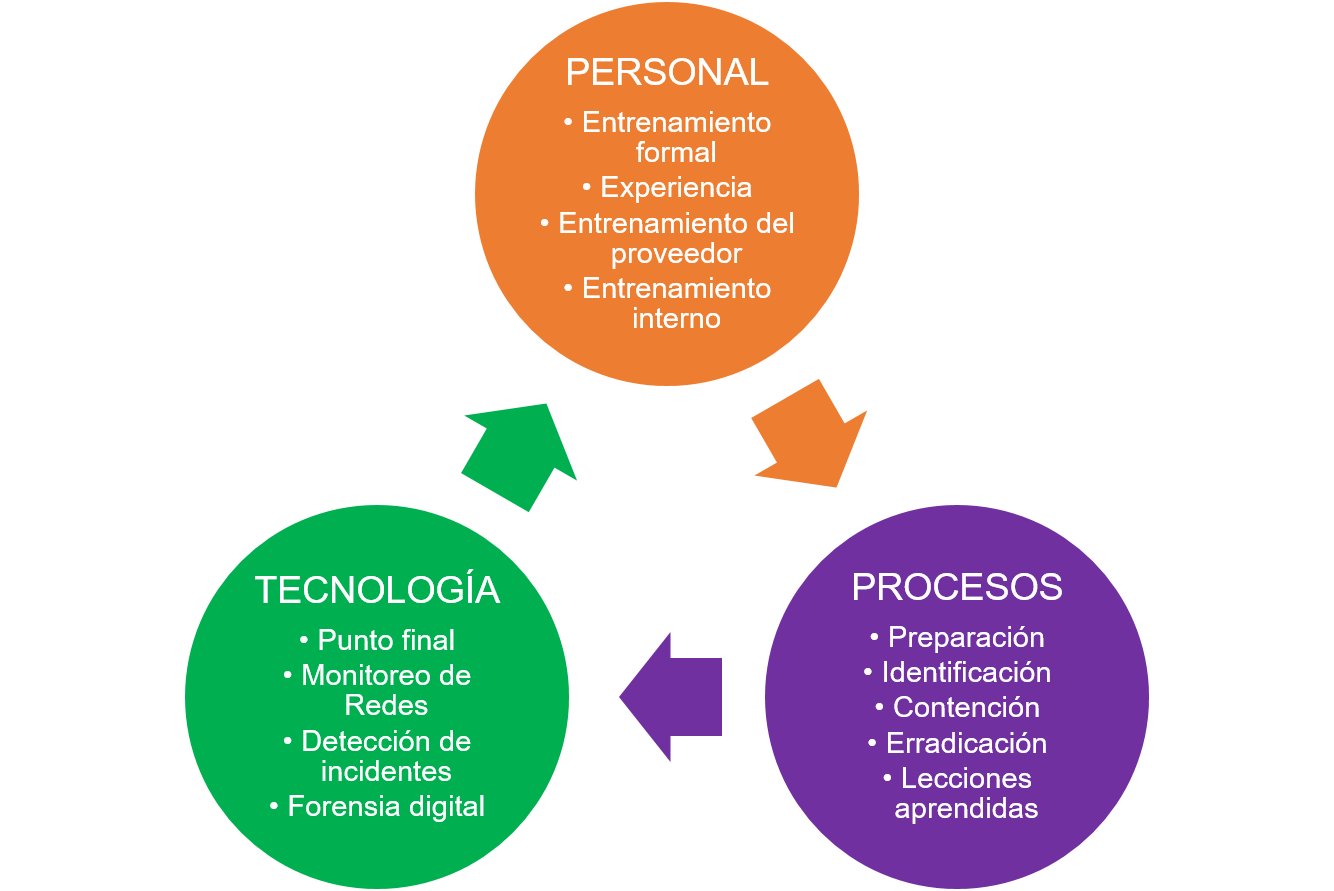
\includegraphics[width=1\textwidth]{./marco_teorico_imagenes/figura_1_pilares.png}
            \caption{Pilares de un CSIRT}
            \label{fig:pilares}
        \end{figure}
        %\par
        \FloatBarrier
        El CSIRT debe tener una perspectiva flexible y escalable para mantener el ritmo de las tácticas de los adversarios, acompañando el crecimiento y evolución de la organización. \par
    \end{section}
    
   \begin{section}{Personal}  
   En cuanto al personal, estos comprenden tanto a los encargados de dar respuesta a los incidentes como a los analistas del CSIRT. Si bien la propia organización puede designar a sus integrantes para asumir estas funciones, existen otras alternativas como la tercerización mediante empresas especializadas que proveen el servicio de Managed Security Service Provider (MSSP) o contratar especialistas en respuesta a incidentes en el caso de una emergencia o un problema complejo. Otra vía consiste en la creación de equipos híbridos compuestos por personal perteneciente a la organización y especialistas externos. \par
    De acuerdo a una encuesta del SANS Institute del año 2014 \cite{sans_1}, el 61\% de las organizaciones relevadas manifestaron haber recurrido a personal de emergencia para cubrir incidentes críticos y el 58 \% tenía un equipo de respuesta propio. Por lo que las organizaciones no siempre cubren sus necesidades con miembros de su propio personal y en algunos casos las tareas recaen por completo en los servicios de terceros. Esto se debe a que, sin importar la estructura del equipo, el personal de un CSIRT debe contar con el entrenamiento necesario para tratar con los cambios en las amenazas a las que se enfrenta. En el Cuadro \ref{table:1} se muestran las responsabilidades y la formación requerida para cada uno de los integrantes de un CSIRT. \par
    
    \begin{table}%[ht]
    \centering
        \begin{tabular}{ | m{10em} | m{16em}| m{11em} | } 
            \hline
            Título profesional & Tarea & Entrenamiento requerido \\ 
            \hline
            Nivel 1 - Analista de alertas & Supervisa continuamente la cola de alertas, monitorea el estado de los sensores y los puntos finales, clasifica las alertas de seguridad y recopila los datos necesarios para iniciar el trabajo de Nivel 2. & Procedimientos de triage de alerta y detección de intrusos. Gestión de redes, información de seguridad y eventos. Capacitación en investigación basada en host. \\ 
            \hline
            Nivel 2 - Analista de respuesta a incidentes & Realiza un análisis profundo de incidentes al correlacionar datos de varias fuentes y determina si un sistema crítico o un conjunto de datos se ha visto afectado. Asesora sobre su remediación. & Análisis avanzado de forensia de redes y basado en host. Procedimientos de respuesta a incidentes, revisiones de registros, evaluación básica de malware e inteligencia de amenazas. \\ 
            \hline
            Nivel 3 - Especialista en la materia & Se trata de un conjunto de especialistas que cubren distintas áreas de un CSIRT. 
            Actúan como “cazadores” de amenazas, sin esperar que se intensifiquen los incidentes. Se encuentra estrechamente involucrado en el desarrollo, ajuste e implementación de análisis de detección de amenazas.
             & Entrenamiento avanzado en detección de anomalías. Entrenamiento específico en herramientas para la agregación y análisis de datos e inteligencia de amenazas. 
            Poseen un conocimiento profundo en áreas como redes, puntos finales, inteligencia de amenazas, forensia e ingeniería inversa de malware, así como la infraestructura de IT subyacente.
            \\ 
             \hline
            Director del CSIRT & Administra recursos para incluir personal, presupuesto, programación de turnos y estrategias para cumplir con los acuerdos de nivel de servicio. Se comunica con la gerencia y sirve como persona de contacto en el caso de incidentes críticos. Proporciona una dirección general para el CSIRT. & Gestión de proyectos, formación en gestión de respuesta a incidentes, habilidades generales de gestión de personas y comunicación institucional.  \\
            \hline %linea final de tabla
        \end{tabular}
        \caption{Integrantes de un CSIRT y sus funciones}
        \label{table:1}
    \end{table}
    \FloatBarrier % obliga a la imagen a renderizarse antes de este punto
        Para organizar el trabajo de los analistas, un CSIRT necesita un director que coordine los múltiples esfuerzos dentro y fuera del equipo. Su responsabilidad es dirigir el trabajo y organizar los recursos con el fin de detectar, investigar y priorizar incidentes que puedan impactar en la organización. Otra de las misiones asignadas al director consiste en desarrollar un modelo de flujo de trabajo e implementar procedimientos operativos estandarizados, para el proceso de manipulación de incidentes, que guíen a los analistas en la clasificación y respuesta apropiada.
        En la Figura \ref{fig:org_csirt} se observa un modelo de organización de un CSIRT.
        
        \begin{figure}[H]
            \centering
            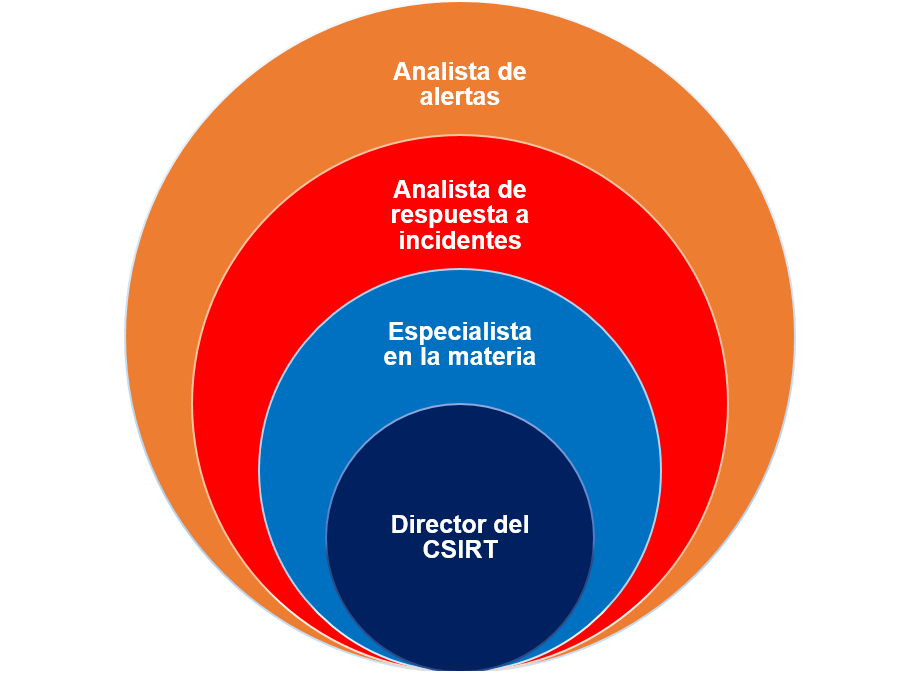
\includegraphics[width=1\textwidth]{./marco_teorico_imagenes/figura_2_org_csirt.png}
            \caption{Organización de un CSIRT}
            \label{fig:org_csirt}
        \end{figure}

   \end{section}
   
   \begin{section}{Procesos}  
        Para estandarizar las acciones que pueden tomar los analistas del CSIRT y asegurar que no se perderán tareas importantes en el camino, es necesario definir procesos repetibles de clasificación de incidentes e investigación. Al crear un flujo repetible de gestión de incidentes, se definen las responsabilidades y acciones de los miembros del equipo: desde la creación de una alerta y evaluación por analistas de nivel 1, hasta el tratamiento del incidente por parte del personal de los niveles superiores. Como consecuencia, la segmentación del proceso permite una gestión eficiente de los recursos del CSIRT. \par
    	Uno de los modelos de procesos de respuesta a incidentes más utilizado es el modelo DOE/CIAC \cite{doe_ciac}, que consiste en seis etapas: preparación, identificación, contención, erradicación, recuperación y lecciones aprendidas.

   \end{section}
   \begin{section}{Tecnología}
        En el núcleo de un CSIRT se encuentran las tecnologías de recolección de datos, agregación, detección, análisis y administración. En cuanto a la recolección, se trata de un sistema de monitoreo que obtiene sus datos a partir de un conjunto variado de fuentes como puntos finales (PC, dispositivos móviles, servidores, etc), redes, generadores de logs y eventos. Como resultado de la disponibilidad de los datos, antes y durante el incidente, los analistas pueden utilizar el sistema de vigilancia como una herramienta de investigación, revisando las actividades sospechosas del incidente en curso. Por otro lado, el sistema de monitoreo puede ser utilizado para generar la respuesta al incidente y potencialmente mitigar sus causas. \par
        Un aspecto importante a considerar es la compatibilidad de las tecnologías empleadas, en particular si la organización ya cuenta con una herramienta de monitoreo existente y se busca incorporar nuevas soluciones para integrarlas a los sistemas en servicio. En la Figura \ref{fig:comp_tech} se ejemplifica la necesidad de compatibilidad entre sistemas y componentes. 
        
        \begin{figure}[H]
            \centering
            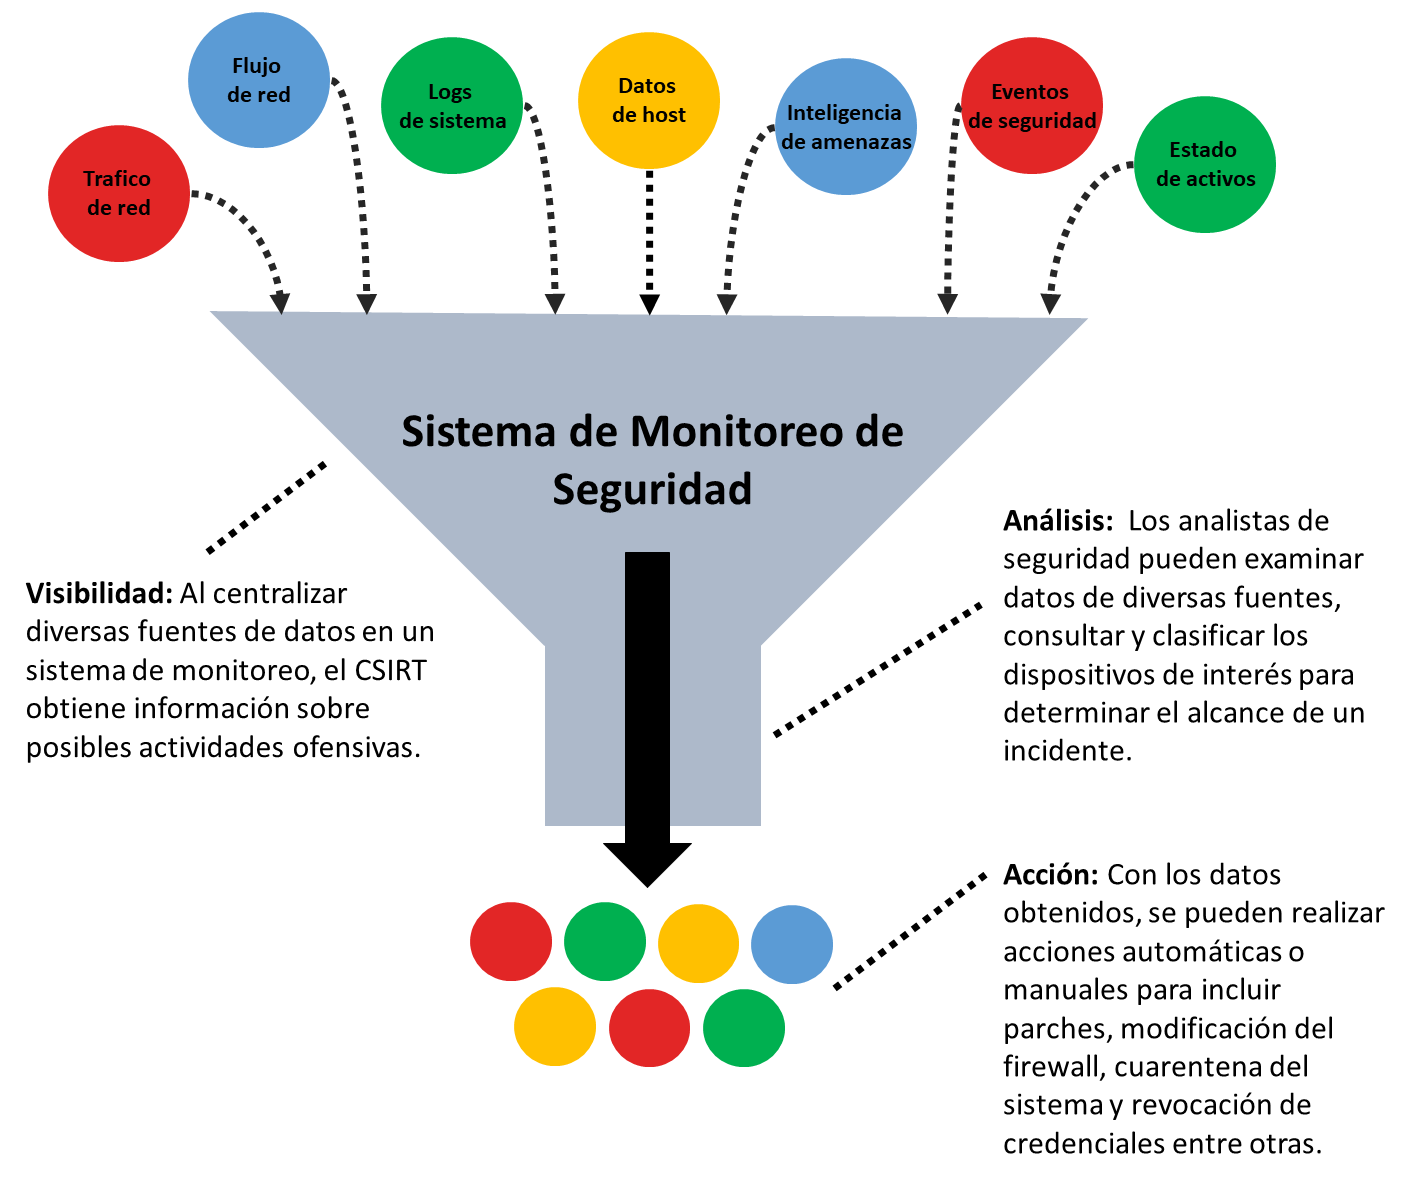
\includegraphics[width=1\textwidth]{./marco_teorico_imagenes/figura_3_compatibilidad_entre_tecnologias.png}
            \caption{Compatibilidad entre tecnologías de detección}
            \label{fig:comp_tech}
        \end{figure}
        \FloatBarrier
        \begin{subsection}{Agregando contexto a los incidentes}
        La incorporación de inteligencia de amenazas y otras informaciones de contexto tales como activos e identidades, contribuye al proceso de investigación del analista de un CSIRT. En determinados casos, la información inicial que está asociada a una alerta puede ser muy limitada, por ejemplo la dirección IP del punto final sospechoso es insuficiente por sí sola para tomar una decisión. \par
        Para que los analistas puedan investigar un incidente, generalmente necesitan más información, por ejemplo los nombres del dueño y de dominio de la máquina, registros DHCP para mapear la IP con el host al momento del incidente, etc. Si el sistema de monitoreo incorpora información de identidad y de los activos de información, entre otros datos de contexto, le permitirá al analista ahorrar tiempo y esfuerzo para priorizar los incidentes y elaborar la respuesta más apropiada.\par

        \end{subsection}
        \begin{subsection}{Definición de conductas normales}
        Dado que es posible observar patrones de comportamiento en usuarios, aplicaciones, infraestructura, redes y dispositivos, es útil establecer una referencia o línea base de la actividad de lo que se considerará un comportamiento normal. Esto facilitará la detección de conductas sospechosas anticipando posibles amenazas. \par
        Un sistema de monitoreo configurado y con una base de referencia adecuada estará en condiciones de enviar alertas confiables al analista de primer nivel. Esto obtiene especial relevancia, ya que de acuerdo al citado informe del SANS Institute del año 2014 \cite{sans_1}, uno de los principales desafíos en la utilización de registros de eventos de seguridad, es la incapacidad de distinguir actividades sospechosas de las normales. La ausencia de una referencia de “normalidad” es un obstáculo común al que se enfrentan las empresas de monitoreo y muchas organizaciones. \par
        La mejor práctica es utilizar plataformas que pueden crear líneas o patrones de referencia mediante el monitoreo de la red y la actividad de los puntos finales durante un periodo de tiempo.
        \end{subsection}
        
        \begin{subsection}{Inteligencia de amenazas}
        Los CSIRT bien establecidos o maduros desarrollan continuamente la capacidad de aprovechar la inteligencia de información proveniente tanto de sus incidentes pasados como de fuentes de inteligencia compartidas. Ejemplos de estas últimas son los proveedores especializados, CSIRT aliados, divisiones policiales de cibercrimen, organizaciones de intercambio de información como la Information Technology - Information Sharing and Analysis Center (IT-ISAC) \cite{it_isac}, etc. \par
        La capacidad de utilizar la inteligencia de amenazas contribuye a mejorar la precisión de la detección. De esta manera, es posible detectar patrones de amenazas ocultas en puntos finales, logs y registros de red, reduciendo las oportunidades de desarrollo de un ataque.
        \end{subsection}
        \pagebreak
        \begin{subsection}{Obstáculos para el manejo eficiente de incidentes del CSIRT}
        Algunos de los obstáculos que deben ser evitados por un CSIRT son aquellos que generan cuellos de botella en el proceso de respuesta a incidentes.  Este proceso que consiste en el traslado de un incidente entre los sucesivos niveles del CSIRT, eventualmente puede generar “ruido blanco”: la presencia de una gran cantidad de alertas de poca importancia y / o falsos positivos. De prolongarse esta situación en el tiempo, se produce un fenómeno llamado “fatiga de alertas” que afecta a los analistas provocando una disminución en sus capacidades de atender incidentes prioritarios. \par
        Al momento de elegir una herramienta de monitoreo, se debe considerar que incluya entre sus características la personalización del umbral de alertas y la posibilidad de combinar distintas alertas en un mismo incidente. Una herramienta de este tipo permite a los analistas clasificar las alertas más rápido, reduciendo las capas de evaluación necesarias antes de que el evento pueda ser confirmado y mitigado. 
        \end{subsection}
   \end{section}
      
   \begin{section}{Ámbitos de actuación de los CSIRT}
        En la actualidad existen en todo el mundo CSIRT pertenecientes a organizaciones que responden a distintos ámbitos de la sociedad y de diferente naturaleza (pública o privada). En términos generales, estos equipos se clasifican dependiendo de la comunidad a la que atienden, diferenciándose entre:
        \begin{itemize}
            \item \textbf{CSIRT para el sector de PYMES:} En este caso, el tamaño de las empresas hace poco viable que las organizaciones de este sector puedan implementar de forma individual las funciones de un CSIRT. Por lo tanto, surge la necesidad de unificar esfuerzos y servicios en un solo equipo capaz de dar soporte a varias empresas. La naturaleza de estos CSIRT puede ser pública o privada, dependiendo del contexto en el que se encuentren estas compañías.
            \item \textbf{CSIRT académico:} El área de responsabilidad de este tipo de equipos se circunscribe a instituciones académicas. Su tamaño, por lo tanto, puede variar dependiendo de las dimensiones de la comunidad, condicionando los servicios que ofrezcan, el modo en que lo hagan y su grado de intervención.
            \item \textbf{CSIRT comercial:} estos centros prestan distintos servicios a cambio de una contraprestación económica. Se trata de empresas especializadas en la industria de la ciberseguridad, que habitualmente utilizan acuerdos de servicios específicos con cada cliente.
            \item \textbf{CSIRT de proveedor:} se centra en los productos o servicios específicos de un proveedor. Su objetivo es proveer servicios y soluciones para eliminar o reducir el impacto negativo de las vulnerabilidades en estos últimos, ya sea un producto tecnológico o un servicio TIC.
            \item \textbf{CSIRT del sector militar:} Prestan servicios a organizaciones militares, con responsabilidades en infraestructuras TIC necesarias para la Defensa. Su comunidad está conformada por las instituciones militares y de entidades estrechamente relacionadas con éstas. Por ejemplo, en nuestro país el Comando Conjunto de Ciberdefensa \cite{fa_comando}, es el encargado de la defensa de la infraestructura de redes y activos de la información de las Fuerzas Armadas.
            \item \textbf{CSIRT para protección de infraestructuras críticas:}  Los CSIRT de este sector se centran principalmente en la protección de las infraestructuras críticas  y de los activos de información asociados. Ejemplos de infraestructuras críticas son las centrales y redes de energía, telecomunicaciones, sistema financiero, sector sanitario, agua, transportes, industria nuclear, etc.
            \item \textbf{CSIRT gubernamental:} Bajo esta denominación se sitúan los equipos cuyo principal objetivo es asegurar la infraestructura TIC de un Gobierno/Estado y los servicios ofrecidos a la población. La Comunidad a la que están dirigidos son las administraciones públicas y sus distintos organismos. Estos CSIRT gubernamentales generalmente forman parte de las instituciones del Estado.
            \item \textbf{CSIRT Nacional:} Este es un equipo con responsabilidad general de coordinación sobre todos los sectores y tiene una amplia responsabilidad sobre prácticamente todos los CSIRT tratados anteriormente. Este centro funciona como punto focal de contacto tanto en el entorno nacional como para requerimientos internacionales. ENISA, la Agencia de Ciberseguridad para la Unión Europea, define en un documento \cite{enisa} elaborado en diciembre de 2009, a este tipo de CSIRT como “aquel que actúa como el Point of Contact (POC) con otros equipos nacionales y/o internacionales. De hecho, podría considerarse como CSIRT  del último recurso, por su papel de coordinación”. Cada nación define la misión de estas unidades y establece sus operaciones, su organización y su imperativo legal en base a las necesidades del país y su comunidad. En Argentina, esta responsabilidad es asumida por la Dirección Nacional de Ciberseguridad \cite{dir_nac_ciber}. 
            \begin{figure}[H]
                \centering
              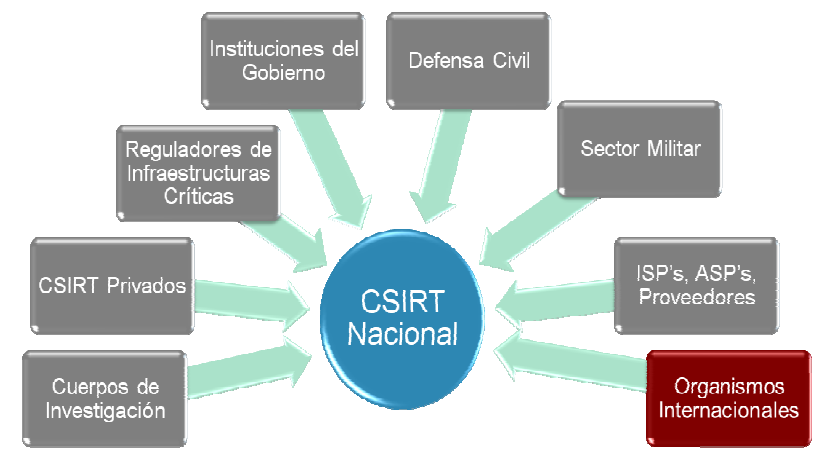
\includegraphics[width=0.8\textwidth]{./marco_teorico_imagenes/figura_4_csirt_nacional.png}
                \caption{CSIRT Nacional como centro de coordinación}
                \label{fig:csirt_nac}
            \end{figure}
            \FloatBarrier
            Frente a esto, todos los CSIRT nacionales tienen un objetivo común, mantener seguras las redes de sus países. De este modo podemos concluir que, aunque cada uno utiliza herramientas y procedimientos diferentes, todos comparten el mismo objetivo:
            \begin{enumerate}
                \item Designar un punto de contacto para la coordinación de la respuesta a incidentes.
                \item Construir y mantener una red de contactos extensa, tanto nacional como internacional.
                \item Monitorización de la situación actual y mejora de la concientización.
            \end{enumerate}
            Es importante destacar que la constitución de un CSIRT nacional o gubernamental, no es la única medida a tener en cuenta en una estrategia de ciberseguridad completa por parte de un Estado. Es una parte importante de la misma teniendo en cuenta, además, que este tipo de equipos deberían asumir la responsabilidad de la Protección de las Infraestructuras Críticas de Información (CIIP) del país.
        \end{itemize}
        \begin{subsection}{Estado de la ciberseguridad en Argentina} 
        Los orígenes de la gestión de la seguridad informática en nuestro país pueden rastrearse en el decreto 856/98 \cite{jef_gab_856_98} y a la Resolución de la Secretaría de la Función Pública (SFP), organismo dependiente de la Jefatura de Gabinete de Ministros, Res SFP 81/99 \cite{sub_tec}. Esta Resolución establece la reorganización de la Subsecretaría de Tecnologías Informáticas y el “Reglamento de Operación del ArCERT", donde se indican los requisitos y condiciones de operación de la Coordinación de Emergencia en Redes Teleinformáticas - ArCERT, y las Políticas de Seguridad del mismo. \par
        El objetivo principal del ArCERT fue coordinar y colaborar en los esfuerzos orientados a elevar los umbrales de seguridad en los recursos y en los sistemas de información en el ámbito de la Administración Pública Nacional (APN). Para esto se estableció una estrategia de coordinación, asesoramiento y capacitación hacia los organismos públicos en la gestión de la problemática de seguridad. \par
        Sus funciones \cite{sub_tec} eran: 
        \begin{enumerate}
            \item Proveer un servicio especializado de asesoramiento en seguridad de redes.
            \item Promover la coordinación entre los organismos de la Administración Pública Nacional para prevenir, detectar, manejar y recuperar incidentes de seguridad.
            \item Centralizar los reportes sobre incidentes de seguridad ocurridos en la APN y facilitar el intercambio de información para afrontarlos.
            \item Actuar como repositorio de toda la información sobre incidentes de seguridad, herramientas, técnicas de protección y defensa.
        \end{enumerate}
        En el marco de las funciones nombradas, el ArCERT realizó actividades de investigación de amenazas y nuevas soluciones disponibles,  divulgación de incidentes y soluciones así como capacitaciones de seguridad en redes y seminarios de actualización periódicos. \par
        El año 2011 marcó el comienzo de un largo proceso de reestructuración de los organismos del Estado Nacional relativos a la ciberseguridad, que incluyó el reordenamiento de estructuras internas, la creación de nuevas dependencias y el reemplazo o absorción de unidades preexistentes por las de nueva formación. Ese mismo año, mediante la resolución de la Jefatura del Gabinete de Ministros, Res JGM Nº 580/2011 \cite{jef_gab_crease} se creó el Programa de Infraestructuras Criticas de Informacion y Ciberseguridad, que declaró como finalidad “Impulsar la creación y adopción de un marco regulatorio específico que propicie la identificación y protección de las Infraestructuras estratégicas y críticas del Sector Público Nacional, los organismos interjurisdiccionales y las organizaciones civiles y del sector privado que así lo requieran”. \par
        En el año 2013 y mediante el artículo 1º de la Disposición Nº 2/2013 \cite{disp_2_2013} de la Oficina Nacional de Tecnologías de Información (ONTI), se creó el Instituto de Ciencias e Ingeniería de Computación - Computer Emergency Response Team (ICIC-CERT) que reemplazó al ArCERT. \par
        Este nuevo CERT heredaba parte de las responsabilidades del original, a la par que otros artículos de la referida disposición creaban nuevos grupos de trabajo especializados que ampliaban las capacidades, funciones y responsabilidades concentradas originalmente en el ArCERT, tales como el grupo ICIC - GAP (Grupo de Acción Preventiva, art. 3º) con funciones similares a las encargadas al ArCERT pero enfocadas a monitorear “los servicios que el Sector Público Nacional brinda a través de la red de Internet y aquellos que se identifiquen como Infraestructura Crítica para la prevención de posibles fallas de Seguridad”, el grupo “ICIC - GICI” (Grupo de Infraestructuras Críticas de Información, art. 4º) especializado en el desarrollo y aplicación de nuevas tecnologías para el monitoreo, simulación y respuesta a incidentes en la red de infraestructuras críticas, establecer prioridades y planes estratégicos para liderar el abordaje de la ciberseguridad para la protección de este tipo de infraestructuras, coordinar la implementación de ejercicios de respuesta ante la eventualidad de un intento de vulneración de estos activos, entre otras. Finalmente, se creó el grupo de trabajo “ICIC - INTERNET SANO” (art. 7º) con el objetivo específico de ocuparse de las tareas de difusión y capacitación que anteriormente le correspondía al ArCERT. En cuanto al programa de infraestructuras críticas, podemos mencionar la adhesión de la Universidad Nacional de Córdoba, cuando el 15 de Julio de 2014, mediante la Resolución 1221 \cite{unc_rec} firmada por el Rector Tamarit, en su artículo N°1 “Hacer lugar a lo solicitado a fS.1 por la Prosecretaría de Informática y, en consecuencia, adherir al "Programa Nacional de Infraestructuras Críticas de Información y Ciberseguridad"...” \par
        El Estado Nacional siguió actualizando sus políticas en los años siguientes, creando nuevos centros de respuesta a incidentes y actualizando la normativa vigente. Algunos de los ejemplos son la creación del Comando Conjunto de Ciberdefensa de las Fuerzas Armadas \cite{fa_comando}, el “MING-CSIRT” \cite{minis_seg} del Ministerio de Seguridad de la Nación, la Dirección Nacional de Ciberseguridad \cite{dir_nac_ciber} y sus correspondientes unidades de gobierno. \par
       \begin{figure}[H]
            \centering
            \subfloat[\centering] {{
\includegraphics[width=5 cm, valign=c]{./marco_teorico_imagenes/figura_5a_comando_conjunto.png}}} %
            \quad
            \subfloat[\centering] {{
\includegraphics[width=5 cm, valign=c]{./marco_teorico_imagenes/figura_5b_csirt_neuquen.png}}} %
            \caption{Insignias de CSIRTS argentinos: (a) corresponde al Comando Conjunto de Ciberdefensa y (b) corresponde al CSIRT de la provincia de Neuquén}
            \label{fig:ciberdef_nqn}
        \end{figure}
        \FloatBarrier
        Por otro lado, los Estados Provinciales, universidades y empresas también han desarrollado e implantado CSIRTs en sus organizaciones. Algunos ejemplos de esto son el “BA-CSIRT”\cite{ba_csirt} de la Ciudad de Buenos Aires, el “CSIRT-NQN”\cite{nqn_csirt} del gobierno de la provincia de Neuquén, “CERT UNLP” \cite{unlp_cert} de la Universidad Nacional de La Plata o el que dispone NIC Argentina \cite{nic_arg} destinado a la infraestructura crítica de DNS. En el caso de las empresas, podemos mencionar a los CSIRT de las redes bancarias Link \cite{red_link} y Banelco\cite{banelco}.
            \begin{subsubsection}{Demanda de ciberseguridad Argentina}
            Nuestro país, de manera análoga a los demás países de la región, ha experimentado un crecimiento exponencial de incidentes de ciberseguridad a lo largo de las últimas dos décadas. Esto afecta a individuos, empresas, universidades, infraestructuras críticas y a los organismos de diferentes niveles del gobierno. Este incremento exponencial en la demanda de ciberseguridad no ha encontrado una respuesta adecuada del Estado Argentino. Un ejemplo lo constituyen los 1590 millones de ataques \cite{iProUP} que sufrió el sistema bancario argentino en el año 2019 o los 187 millones de ciberataques entre enero y marzo del 2020 con un incremento del 131\% solo para el mes de marzo, según la plataforma “Fortinet Threat Intelligence Insider Latin America” \cite{fortinet}. \par 
            En la Figura \ref{fig:cant_intentos} se observan las diez amenazas más frecuentes y la cantidad de ataques producidos en Argentina por ellas, en el periodo comprendido entre los meses de abril y junio de 2020. Los tres primeros corresponden al troyano de puertas traseras “DoublePulsar Backdoor”, negociación de cifrados SSL anónimos e intentos de ataque contra una vulnerabilidad de divulgación de información en el servidor SMB de Microsoft Windows. La fuente es un informe de Fortinet Threat Intelligence Insider Latin America \cite{fortinet}.\par
            \begin{figure}[H]
            \centering
            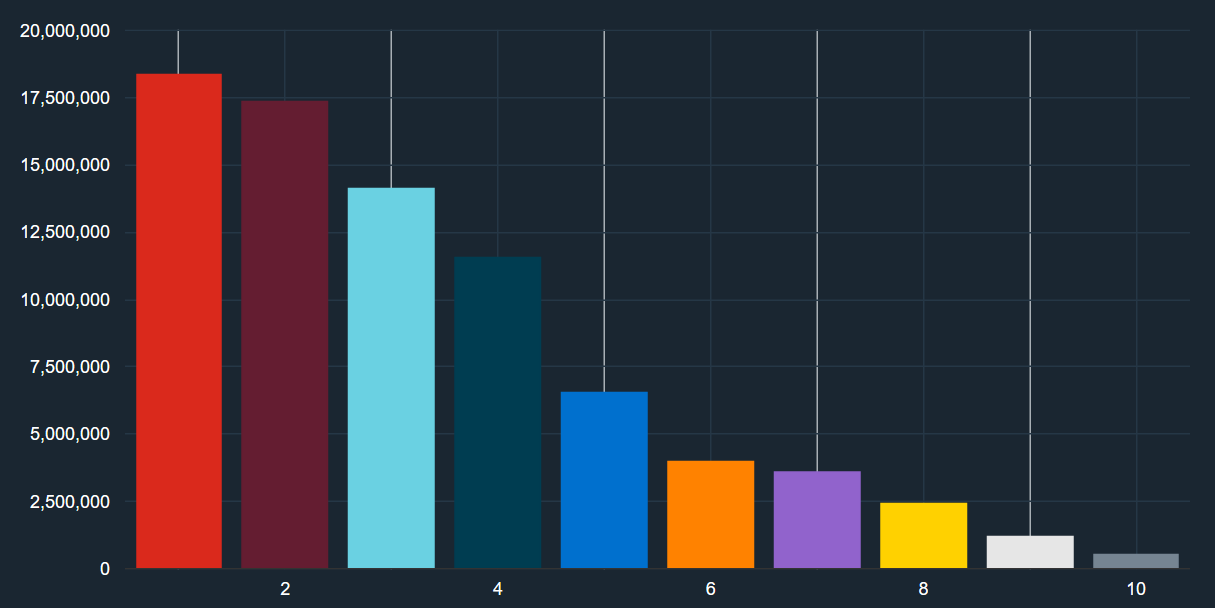
\includegraphics[width=1\textwidth]{./marco_teorico_imagenes/figura_6_cant_intentos_intrusion.png}
            \caption{ Cantidad de intentos de intrusión según la amenaza. Abril - Junio de 2020}
            \label{fig:cant_intentos}
        \end{figure}
        \FloatBarrier
        Hay informes del gobierno nacional \cite{panorama} disponibles desde el 2016 que anticipan esta tendencia, en particular el Ministerio de Modernización indicó que el país registró 5.400 millones de dólares en pérdidas atribuidas a incidentes de ciberseguridad. Esto representa el 1\% del PBI \cite{pbi} del mismo año. La Figura \ref{fig:porcentaje_tipos} del mencionado informe muestra los tipos de incidentes más frecuentes del año 2016 \par
        \begin{figure}[H]
            \centering
            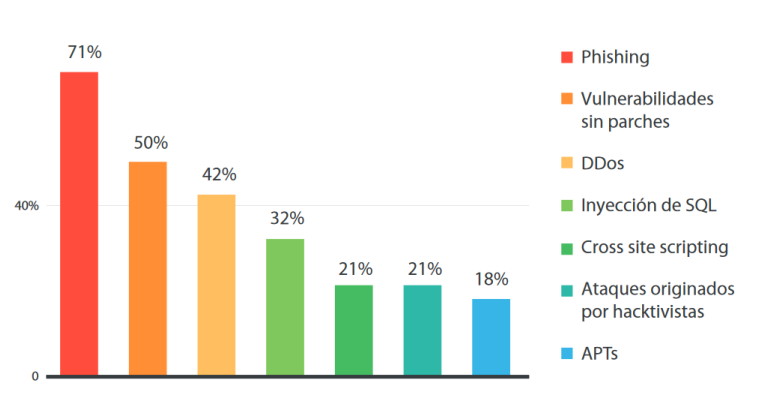
\includegraphics[width=1\textwidth]{./marco_teorico_imagenes/figura_7_tipos_de_incidentes.png}
            \caption{Porcentaje de tipos de incidentes durante 2016}
            \label{fig:porcentaje_tipos}
        \end{figure}
        \FloatBarrier
        Este costo, enorme tanto en relación a la producción nacional como en forma cuantitativa, resalta la necesidad cada vez más importante de desarrollar políticas públicas activas en forma de inversiones en la ampliación de las capacidades de análisis y respuesta a amenazas de ciberseguridad en los organismos de la Administración Pública. \par
        Resulta por lo tanto, necesaria la promoción de iniciativas privadas junto a la concientización de los riesgos existentes, el fomento de investigaciones académicas y la formación de recursos humanos capaces de afrontar estos desafíos, junto a una legislación adecuada y actualizada, para responder al constante aumento de amenazas y complejos escenarios que implica la creciente actividad en línea de industrias, organismos del Estado, comercio y desarrollo de la sociedad en Internet. \par

            \end{subsubsection}
        \end{subsection}
   \end{section}

    \begin{section}{SIEM: Definición y funciones}
    Las capacidades que ofrece un CSIRT para las organizaciones, en términos de prevención y mitigación de incidentes informáticos, se basan en los tres pilares mencionados en las secciones anteriores: el personal, la tecnología y los procesos. \par
    En cuanto a la tecnología, es la que permite llevar a cabo las tareas de recolección de datos, agregación, detección, análisis y administración. Estas tecnologías se encuentran dentro del marco operacional del Security Information and Event Management (SIEM) como entidad dentro de la estructura de organización de un CSIRT. \par
    El proceso de monitoreo de la seguridad de una red de datos compleja requiere recopilar diferentes tipos de datos para detectar, verificar y contener acciones ofensivas. Las tecnologías del SIEM proporcionan informes en tiempo real y análisis de eventos de seguridad a largo plazo, como se muestra en la Figura 8. Todo esto ayuda a la tarea de un analista de ciberseguridad cuando debe verificar acciones ofensivas sobre la red de una organización. \par
    El término SIEM fue acuñado en 2005 por los analistas Amrit Williams y Mark Nicolett de la compañía estadounidense Gartner \cite{def_siem}, una empresa especializada en investigación y consultoría de incidentes de seguridad, unificando los acrónimos en inglés SIM (security information management) y SEM (security events management) para describir metodologías muy similares pero ligeramente diferentes de ciberseguridad. Esta superposición de tareas hizo evidente que un nuevo término podría englobar ambos conjuntos de funciones, con el fin de disponer de un único acrónimo que pudiese identificar a una plataforma capaz de resolver los objetivos de los sistemas predecesores. \par
    De esta manera, el nuevo acrónimo SIEM significa Administración de Eventos de Seguridad de la Información, por sus siglas en inglés. Como plataforma que combina las funciones de los sistemas anteriormente descritos, sus capacidades comprenden la siguiente lista de tareas:
    \begin{itemize}
        \item Recolectar, analizar y presentar de manera eficiente datos relacionados a la seguridad.
        \item Análisis en tiempo real de eventos de seguridad.
        \item Generar reportes y almacenar datos relacionados a la seguridad.
        \item Administración de niveles y tipos de acceso e identidad.
        \item Auditoría de registros.
        \item Respuesta a incidentes y operaciones de seguridad.
    \end{itemize}
    Como se puede observar en la Figura \ref{fig:flujo_datos_siem}, para cumplir con las tareas anteriormente descritas, un SIEM obtiene su información de diversas fuentes:
    \begin{itemize}
        \item Inteligencia de Amenazas, identidades y logs: la revisión de amenazas pasadas y la inteligencia compartida por otras organizaciones aliadas contribuyen a detectar más rápido patrones anormales de comportamiento.
        \item Telemetría de Netflow: es un protocolo de recopilacion de informacion del flujo de red IP.
        \item Captura de paquetes: replicación de paquetes de información con el fin de correlacionar posibles amenazas en el flujo de red.
        \item Dispositivos Antimalware: componentes especializados en la detección de malware, localizados en puntos finales.
        \item IDS (HIDS y NIDS): Sistemas de detección de intrusiones, orientados a redes (NIDS) o puntos finales (HIDS).
        \item Firewalls: software que bloquea y filtra conexiones con origen desde el sistema hacia el exterior y viceversa.
        \item IPS: Sistema de protección de intrusiones. Ofrecen protección activa frente a comportamientos inusuales ya que pueden tomar acciones programadas para evitar un intento de intrusión.
        \item Syslog: Syslog es un protocolo para el tratamiento de logs en un formato estandarizado, empleado fundamentalmente en el monitoreo de la integridad de servidores.
    \end{itemize}
      \begin{figure}[H]
            \centering
            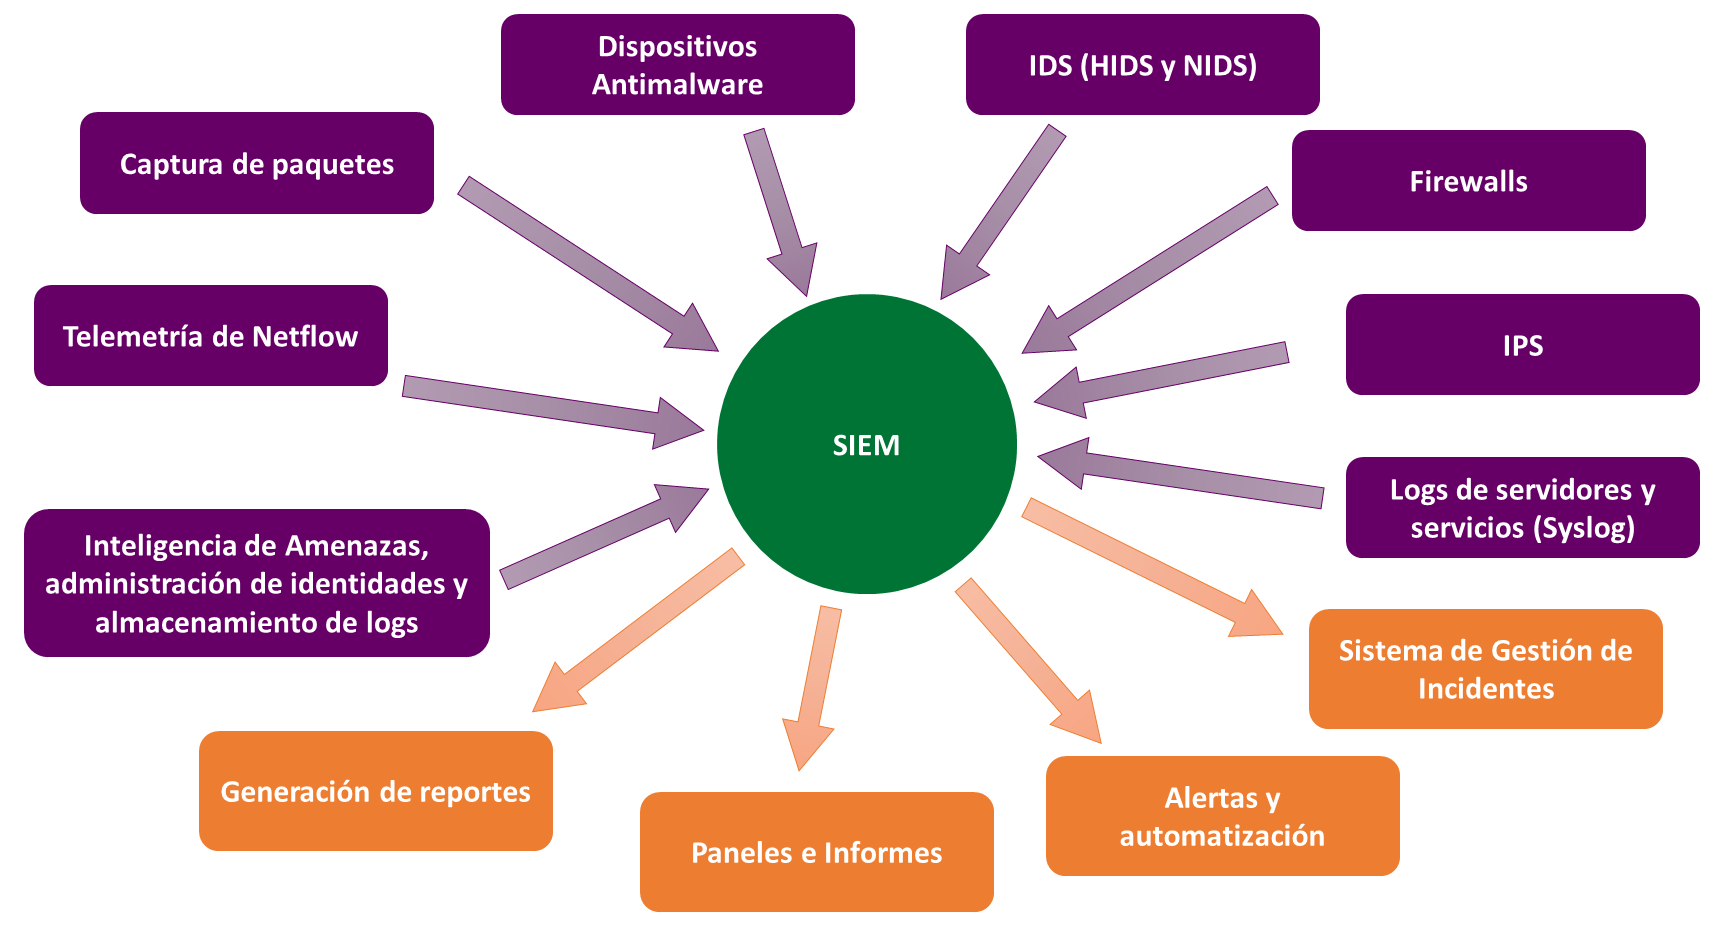
\includegraphics[width=1\textwidth]{./marco_teorico_imagenes/figura_8_datos_de_un_siem.png}
            \caption{Funciones y flujos de datos de un SIEM}
            \label{fig:flujo_datos_siem}
        \end{figure}
        \FloatBarrier
        La secuencia del tratamiento que recibe la información dentro un SIEM está representada en la Figura \ref{fig:procesos_siem}, donde se muestran los cuatro pasos que forman el proceso de respuesta a incidentes del SIEM. La secuencia se detalla a continuación:
        \begin{itemize}
            \item Paso 1: inicialmente es necesario recolectar datos provenientes de diversas fuentes, tales como sistemas IDS, firewall, syslog, switches (protocolos SNMP), entre otros. Como estos datos tienen formatos disímiles entre sí, es necesario un posterior proceso de normalización.
            \item Paso 2: a medida que los datos arriban al SIEM, es necesario someterlos a un proceso de normalización. Este proceso consiste en extraer la información contenida en los distintos mensajes, para almacenarla en un formato estandard. Con el objetivo de reducir el volumen de almacenamiento, la información resultante es sometida a un proceso de agregación, que separa los datos importantes de los secundarios.
            \item Paso 3: es posible analizar los datos resultantes en busca de patrones de actividad inusual. Esta búsqueda se puede realizar de manera manual por un analista o en forma autónoma en el caso de disponer de herramientas  que utilicen inteligencia de amenazas.
            \item Paso 4:  con los resultados del análisis del paso anterior, es posible determinar la existencia de un intento de intrusión u otros tipos de incidentes. De confirmarse este último caso, es posible enviar alertas a los responsables de tomar decisiones para mitigar el incidente.
        \end{itemize}
    \begin{figure}[H]
            \centering
            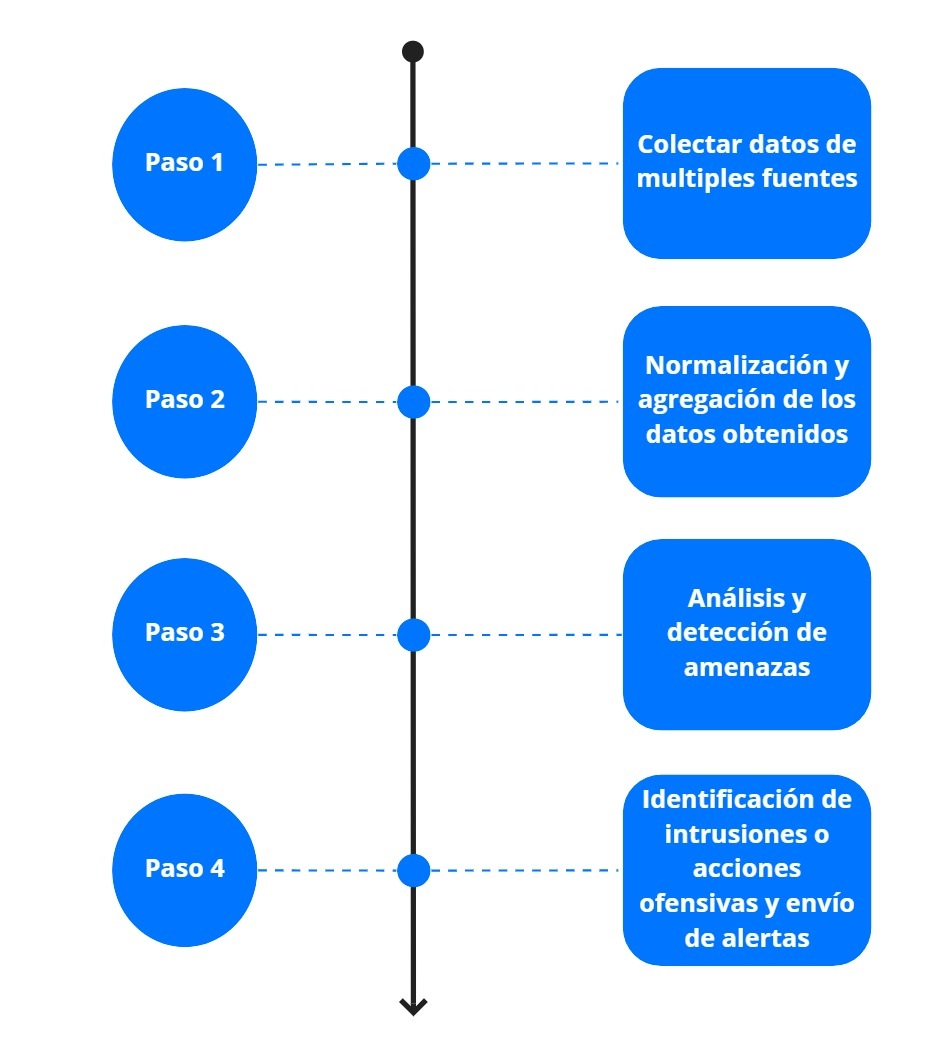
\includegraphics[width=1\textwidth]{./marco_teorico_imagenes/figura_9_procesos_de_un_siem.jpg}
            \caption{Proceso de identificación y respuesta a incidentes de un SIEM}
            \label{fig:procesos_siem}
        \end{figure}
        \FloatBarrier    
        El objetivo, por lo tanto, de un sistema SIEM dentro del CSIRT es concentrar la información proveniente de múltiples fuentes independientes, procesar los datos y realizar un análisis centralizado.
    \end{section}
    \pagebreak
    \begin{section}{Soluciones disponibles}
    Las principales soluciones que existen en el mercado, sean gratuitas, de software libre, pagas o de código propietario,  se presentan a continuación.\par
    En primer lugar se realizó un relevamiento en sitios especializados y de referencia para el mercado mundial, con el objetivo de identificar las soluciones comerciales disponibles, que actualmente dominan el mercado global de SIEM . En el sitio web de Gartner \cite{ranking} se encontró un listado de los productos ordenados por valoración de los usuarios de dicha página. El resultado de los diez primeros productos junto a sus desarrolladores, se muestra en el Cuadro \ref{table:2}. \par
    \begin{center}
        \begin{table}[H]
        \centering
        \begin{tabular}{ | m{4em} | m{22em}| m{12em} | }
            \hline
            Posición & Nombre de la solución & Empresa desarrolladora \\ 
            \hline
            1) & QRadar SIEM\cite{qradar} & IBM. \\ 
            \hline
            2) & ManageEngine ADAudit Plus\cite{adaudit} & ManageEngine. \\ 
            \hline
            3) & LogRhythm NextGen SIEM Platform\cite{logrhythm}
             & LogRhythm
            \\ 
             \hline
            4) & LogPoint - SIEM\cite{logpoint} & LogPoint  \\
             \hline
            5) & McAfee Enterprise Security Manager\cite{enterprise} & McAfee  \\
             \hline
            6) & ArcSight Enterprise Security Manager (ESM)\cite{arcsight} & Micro Focus  \\
             \hline
            7) & InsightIDR\cite{insight} & Rapid7  \\
             \hline
            8) & Elastic (ELK) Stack\cite{elastic} & Elastic  \\
             \hline
            9) & Splunk Enterprise\cite{splunk} & Splunk  \\
             \hline
            10) & Exabeam Security Management Platform\cite{exabeam} & Exabeam \\
            \hline %linea final de tabla
        \end{tabular}
        \caption{Ranking Gartner \cite{ranking} de soluciones SIEM 2020}
        \label{table:2}
    \end{table}
    \end{center}
    \FloatBarrier
    En base a la información recolectada, se procedió a clasificar las herramientas bajo el criterio de la disponibilidad del código: propietarias o libres y el resultado se muestra en el Cuadro \ref{table:3}.
        \begin{table}[h]
        \begin{tabular}{ | m{22em}| m{17em} | } 
            \hline
            Soluciones Pagas y Propietarias & Soluciones Libres y Gratuitas  \\ 
            \hline
            Splunk\cite{splunk} &  \\ 
            
            McAfee Enterprise Security Manager\cite{enterprise} &  \\
            
            AlienVault USM\cite{alienvault_usm} & Graylog\cite{graylog} \\ 
             
            QRadar SIEM \cite{qradar} & Elastic (ELK) Stack\cite{elastic}  \\
             
            ManageEngine ADAudit Plus\cite{adaudit} & AlienVault OSSIM\cite{alienvault_ossim}  \\
             
            LogRhythm NextGen SIEM Platform\cite{logrhythm} & Security Onion\cite{sonion}  \\
             
            LogPoint - SIEM\cite{logpoint} & Sweet Security\cite{sweet_security}  \\
             
            ArcSight Enterprise Security Manager (ESM)\cite{arcsight} &   \\
             
            InsightIDR\cite{insight} &   \\
             
            \hline %linea final de tabla
        \end{tabular}
        \caption{Ranking Gartner \cite{ranking} de soluciones SIEM 2020}
        \label{table:3}
    \end{table}
    
    \pagebreak
    
    \begin{subsection}{Soluciones comerciales}
    
        En nuestro análisis de las soluciones comerciales disponibles, se decidió describir la situación del mercado internacional en función de los siguientes criterios: 
        Usuarios (descritos a través de los sectores industriales a los que pertenecen), la distribución geográfica de los usuarios a nivel global y luego repetimos el análisis con un énfasis en América Latina. \par 
        Respecto de los sectores industriales que hacen uso de sistemas de ciberseguridad y generan demandas de nuevas soluciones, se observó que el sector financiero a nivel mundial es el que lidera el consumo de soluciones SIEM, con la mayoría de los desarrolladores teniendo como clientes principales a empresas y organizaciones de este sector. Esto se explica dado el alto nivel de digitalización de la banca y los servicios financieros, que por su masividad y naturaleza son objetivos prioritarios para cualquier atacante en el ciberespacio. \par
        Finalmente, se hizo una comparación por características entre los principales productos SIEM del mercado internacional, en base a las revisiones de sus usuarios en distintos medios, en particular se tuvo referencia a las publicaciones de “Gartner”\cite{ranking} y “Markets \& Markets”\cite{markets_markets}. 
        Los resultados se encuentran en la Figura \ref{fig:tabla_valoracion}.\par
        %\textfloatsep
        \protect
         \begin{figure}
            \centering
            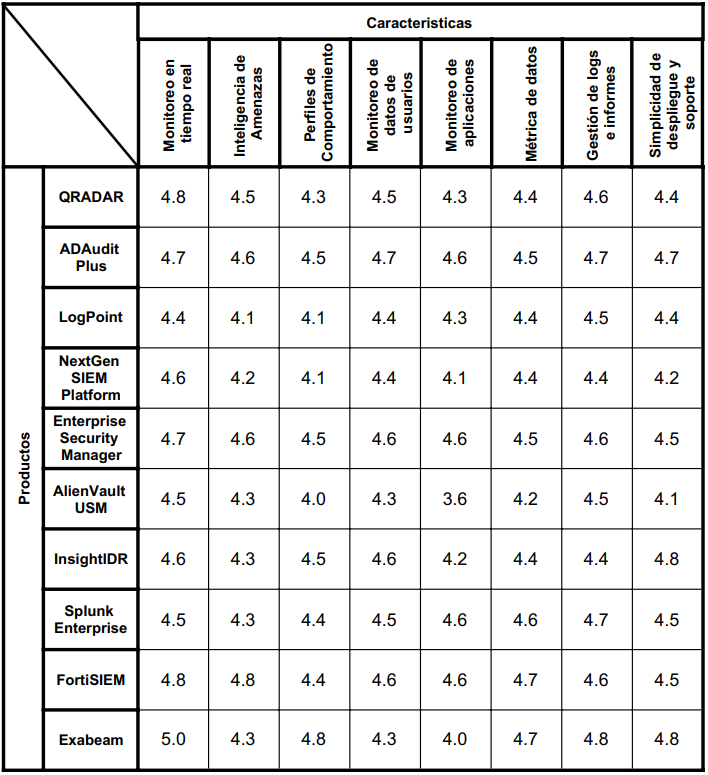
\includegraphics[width=1\textwidth]{./marco_teorico_imagenes/tabla_3_valoracion.png}
            \caption{Valoración de las características}
            \label{fig:tabla_valoracion}
        \end{figure}
        \FloatBarrier
        En la figura comparativa \ref{fig:tabla_valoracion} se observó que FortiSIEM y ADAudit Plus, de las compañías Fortinet\cite{fortisiem} y ManageEngine\cite{adaudit} respectivamente, son las soluciones mejor valoradas.
        \begin{figure}[H]
        \centering
        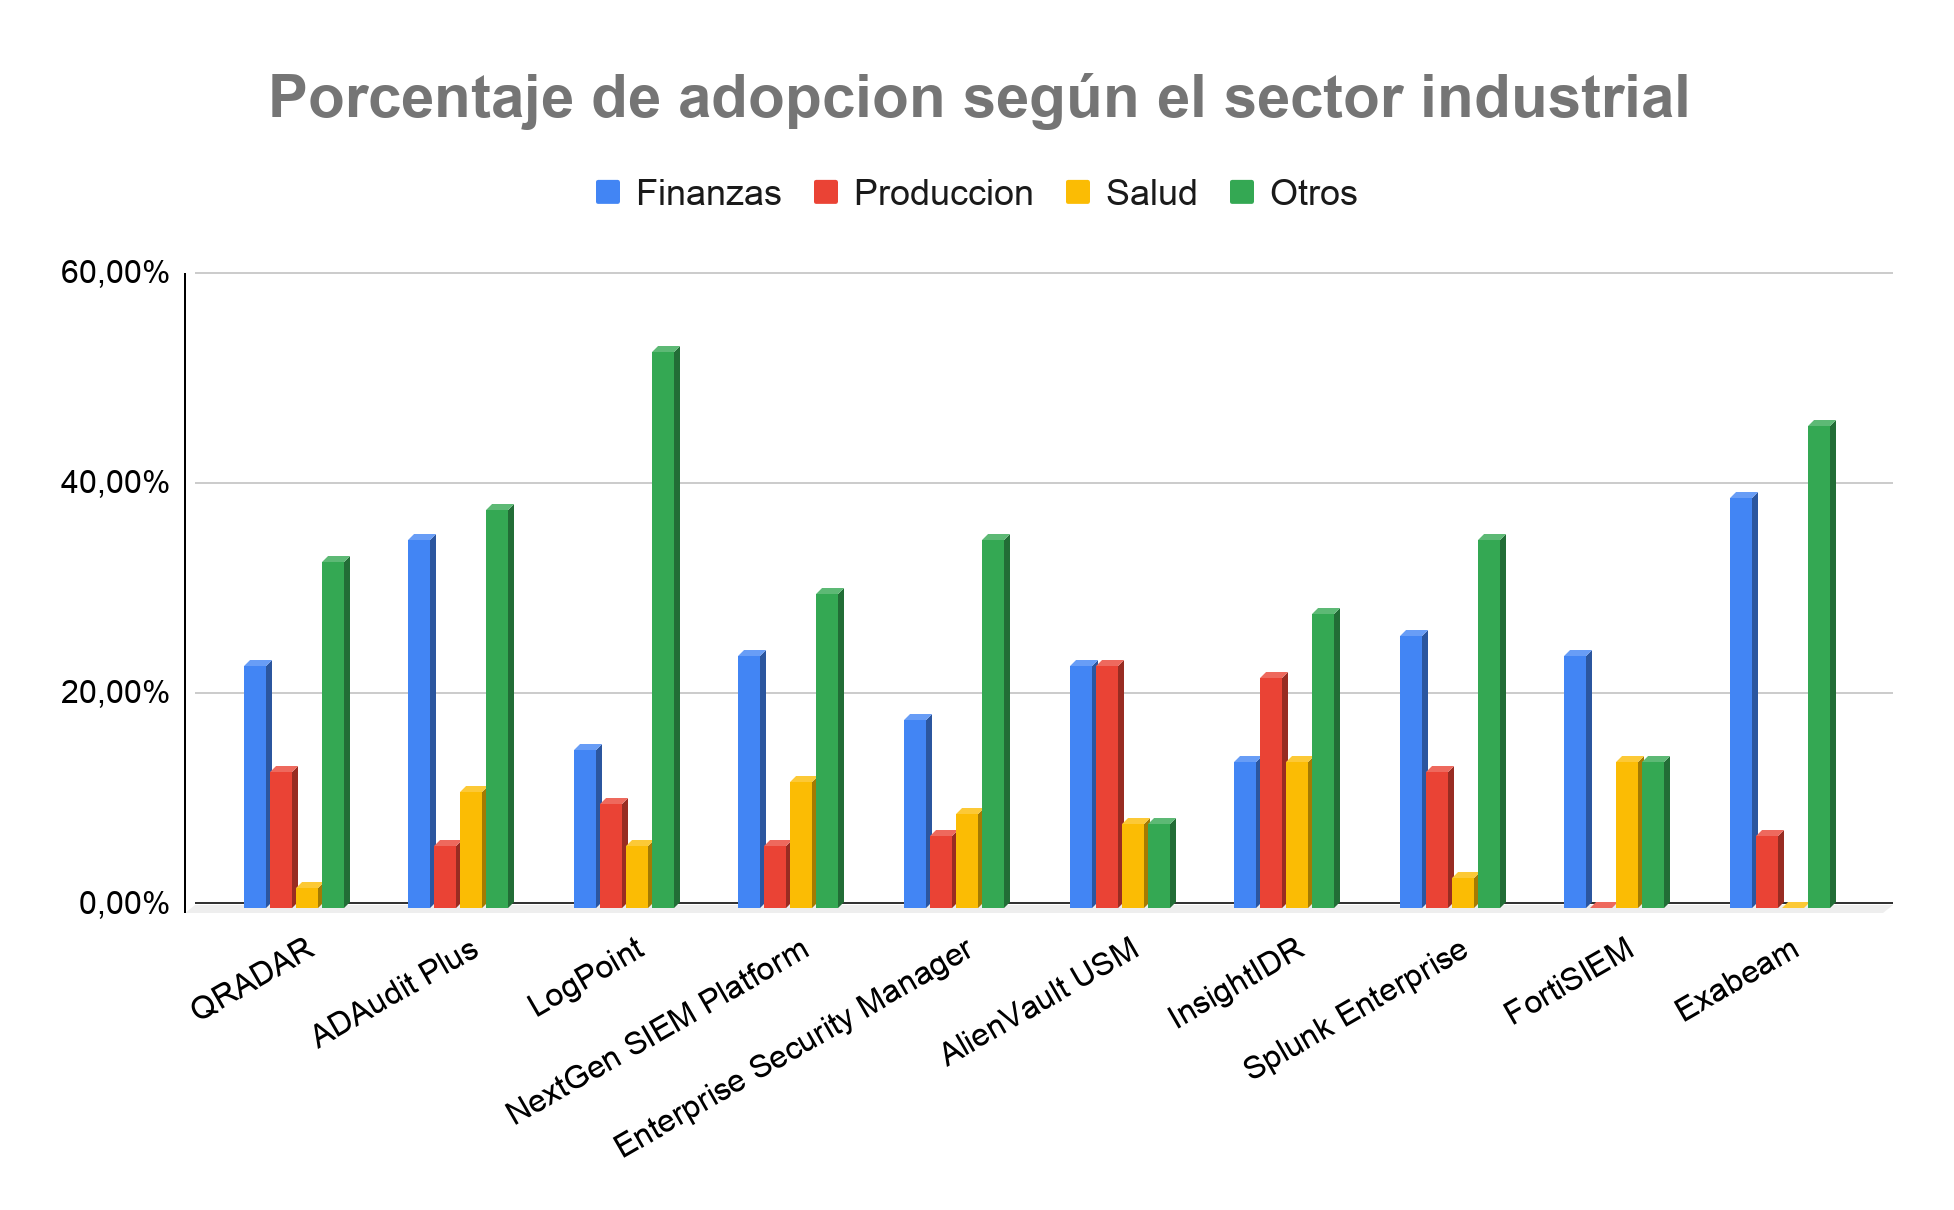
\includegraphics[width=1\textwidth]{./marco_teorico_imagenes/figura_10_porcentaje_sector_ind.png}
        \caption{Porcentaje de adopción según el sector industrial}
        \label{fig:sector_industrial}
        \end{figure}
        \FloatBarrier
       
        En las Figuras \ref{fig:sector_industrial} y \ref{fig:area_geografica_mundial} se aprecia que el sector financiero es el principal demandante de estas soluciones a nivel global, seguido por las industrias manufactureras y de salud. Los sectores industriales se destacan con diferencia respecto al resto en términos de adopción de soluciones SIEM. Esto se debe a que la automatización de la industria primero y su evolución al actual modelo de “industrias 4.0” \cite{industrias_4}, con cadenas de producción, montaje y ensamble distribuidas geográficamente alrededor del globo, implica uso masivo de sensores, redes y datos intrínsecos a cada fase de producción. Esto produjo la necesidad de contar con soluciones de ciberseguridad para evitar incidentes que impliquen el posible robo de información crítica o secretos industriales. De manera análoga al sector manufacturero, las clínicas, hospitales \cite{CCN_CERT} y centros de salud han sufrido el impacto de la digitalización de sus procesos tanto en el hardware médico, el almacenamiento y distribución de la información como en la protección de los sensibles datos privados de los pacientes y la estricta normativa que los regula. \par
        \begin{figure}[H]
            \centering
            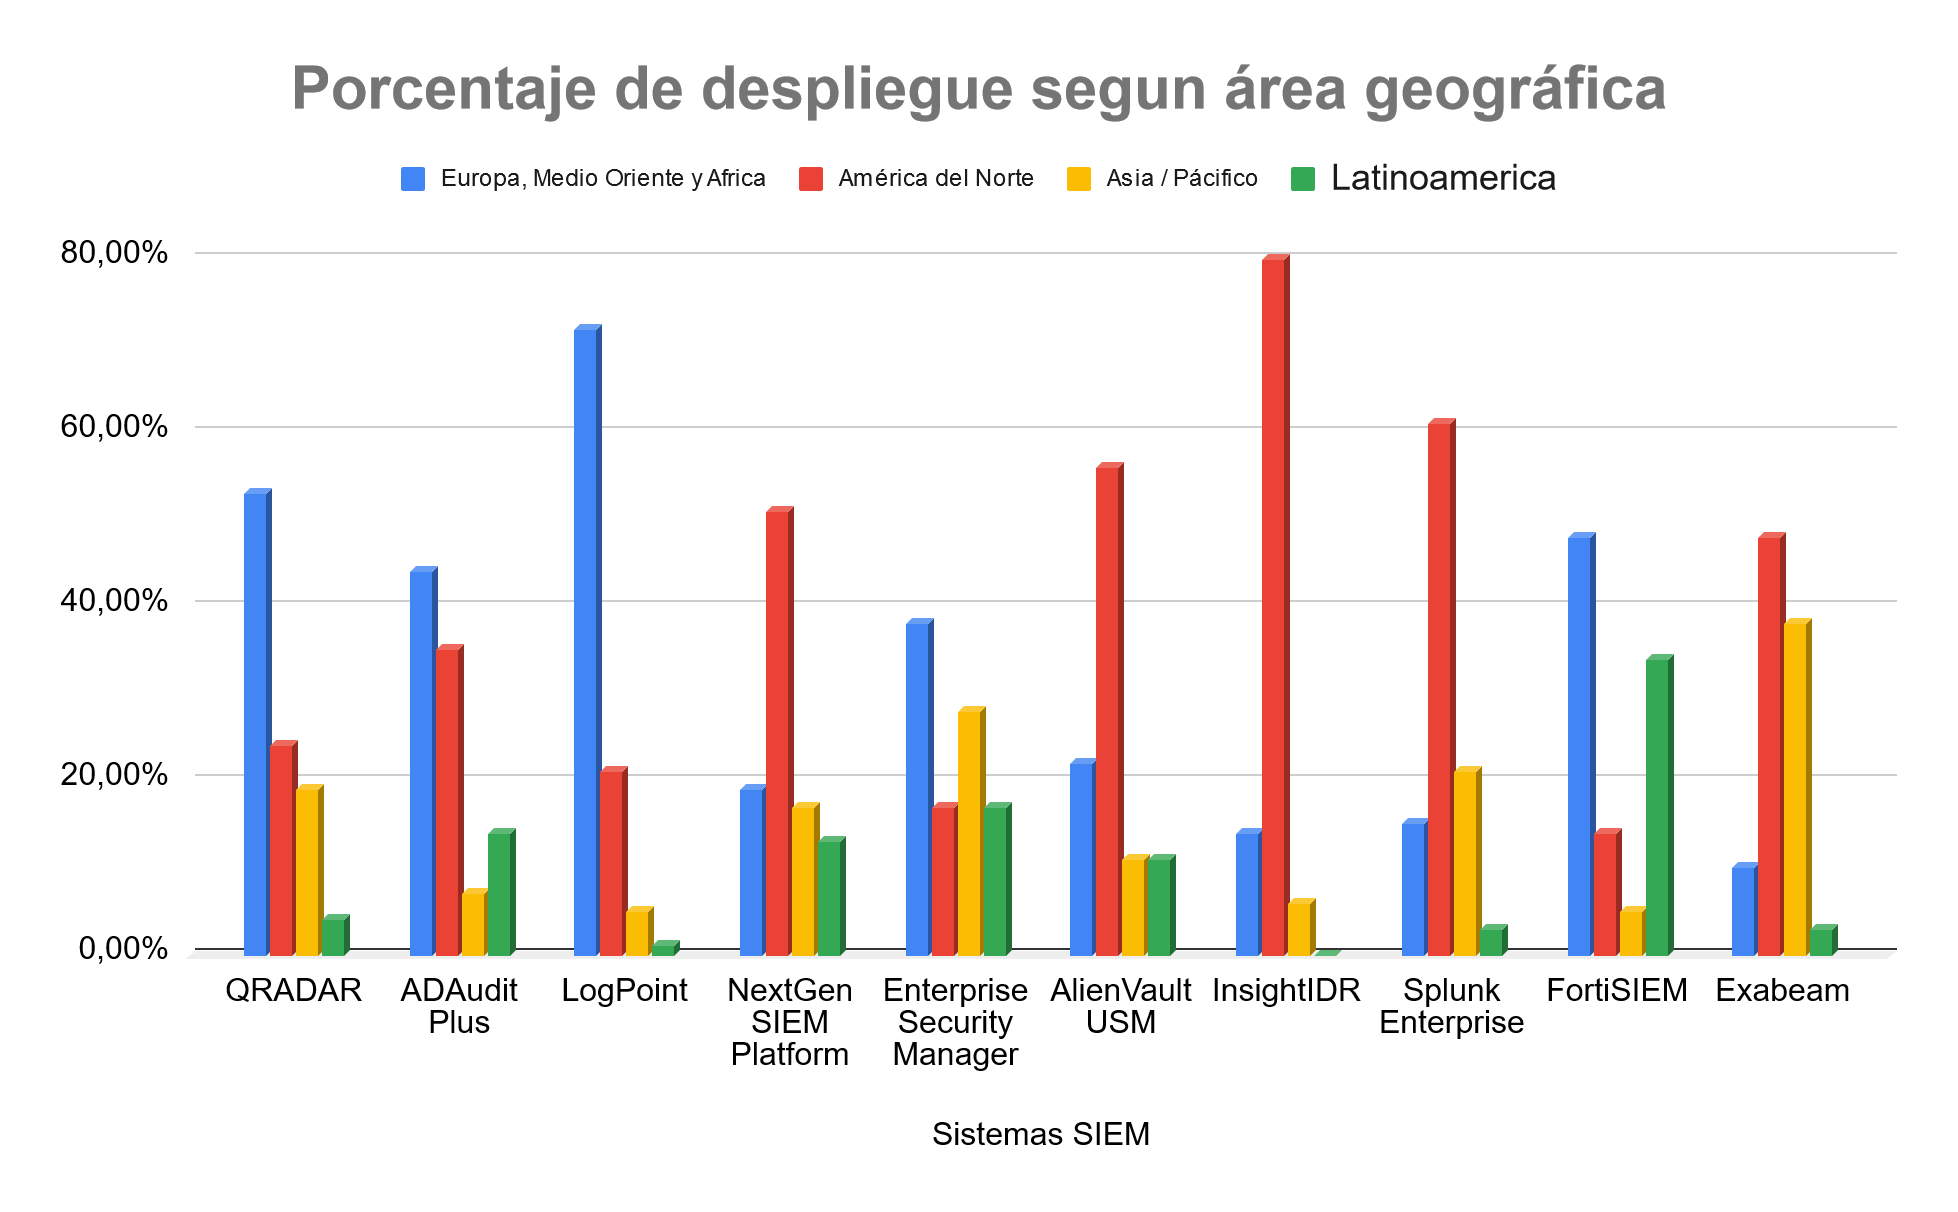
\includegraphics[width=1\textwidth]{./marco_teorico_imagenes/figura_11_porcentaje_area_geografica.png}
            \caption{Porcentaje de despliegue según área geográfica}
            \label{fig:area_geografica_mundial}
        \end{figure}
        \FloatBarrier
        \vspace{-0,5cm}
        En la Figura \ref{fig:area_geografica_mundial} se observa que las soluciones QRADAR\cite{qradar}, LogPoint\cite{logpoint} y FortiSIEM\cite{fortisiem} concentran su demanda en Europa, Medio Oriente y África. En el continente americano existe un contraste entre los mercados de América del Norte y de América Latina. En el norte del continente la mayor parte del mercado es atendido por las soluciones de Enterprise Security Manager\cite{enterprise}, InsightIDR\cite{insight} y AlienVault USM\cite{alienvault_usm}, mientras que la plataforma FortiSIEM es la preferida en Iberoamérica. \par
        \begin{figure}[H]
            \centering
            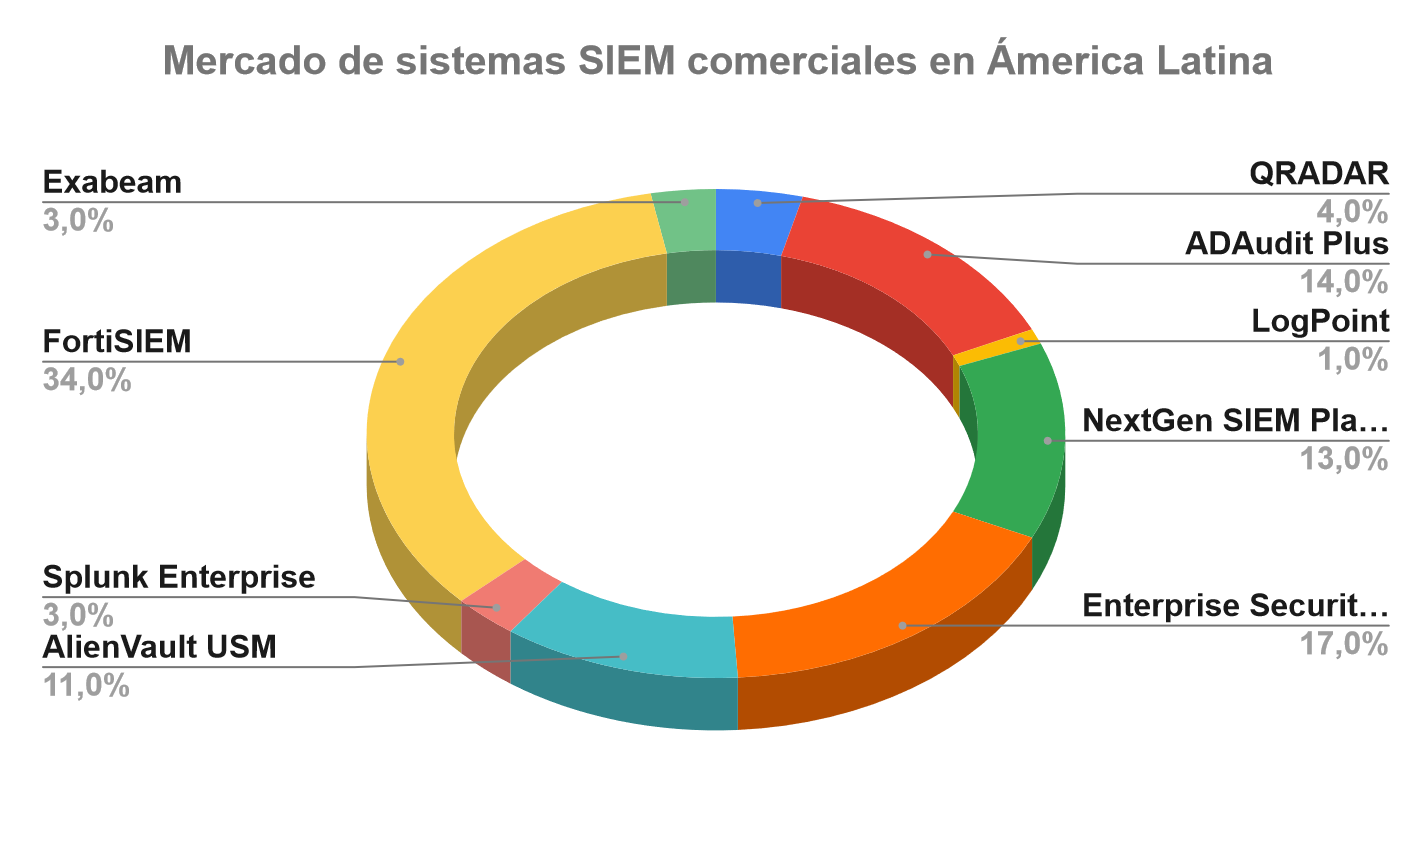
\includegraphics[width=1\textwidth]{./marco_teorico_imagenes/figura_12_comercial_america_latina.png}
            \caption{mercado de sistemas SIEM comerciales en América Latina}
            \label{fig:comercial_latam}
        \end{figure}
        \FloatBarrier
        Sobre nuestra región, en la Figura \ref{fig:comercial_latam} se observó que FortiSIEM acapara el 34 \% del mercado, seguido de Enterprise Security Manager, ADAudit Plus y NextGen SIEM Platform con un 17, 14 y 13 \% del mercado, respectivamente.
        \end{subsection}
        
        \begin{subsection}{Soluciones gratuitas y de código abierto}
        Como consecuencia del relevamiento de las soluciones libres que se encuentran disponibles, se observó que la oferta de productos que cubren estas necesidades es acotada. Incluso en algunos casos, hay proyectos que se encuentran en estado de abandono, como por ejemplo Sweet Security[39]. Este proyecto no cuenta con soporte desde el año 2017. Por otro lado, las versiones abiertas de productos propietarios presentan serias limitaciones respecto de su equivalente comercial, lo que dificulta su consideración como alternativa viable para una organización. \par
        Sin embargo, existen soluciones íntegramente libres capaces de cumplir adecuadamente las misiones de un SIEM, constituyendo una opción válida y competitiva frente a los principales productos comerciales.\par
        Al igual que en el caso de los productos comerciales, se realizó un análisis sobre los sectores industriales a nivel mundial donde predominan las soluciones gratuitas. Como resultado, se observó un uso intensivo en las áreas de servicios IT, esto se debe a que en estas áreas predominan empresas desarrolladoras de tecnología de la información y entes gubernamentales, por lo que en ambos casos cuentan con el personal y recursos necesarios para modificar las soluciones a la medida de sus objetivos e infraestructura. En la Figura \ref{fig:sector_industrial_sol_libre} se puede observar el porcentaje de adopción por área en la industria.\par
        
        \begin{figure}[H]
            \centering
            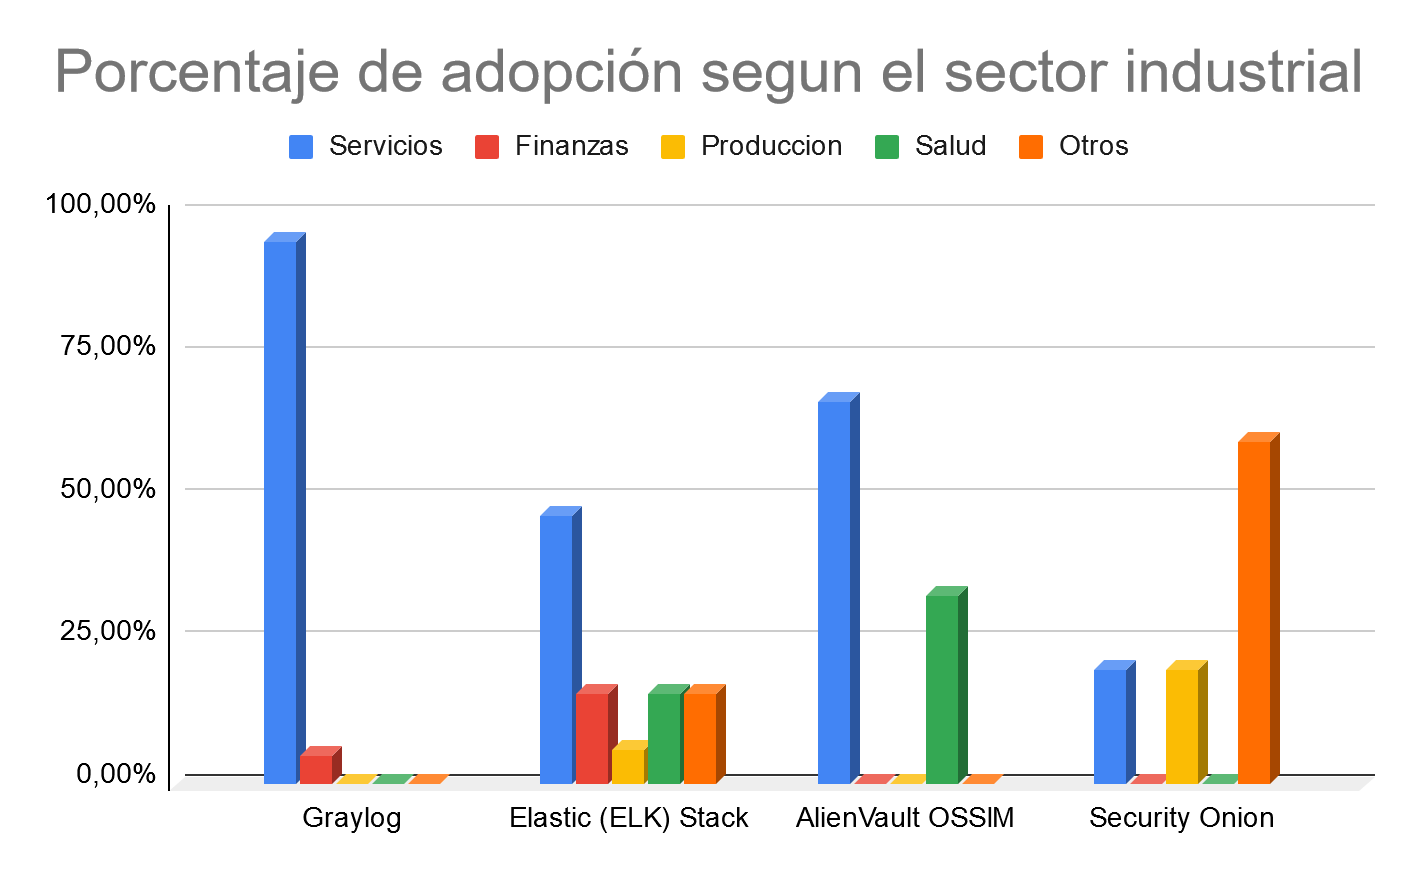
\includegraphics[width=1\textwidth]{./marco_teorico_imagenes/figura_13_ sol_libres_sector_ind.png}
            \caption{Porcentaje de adopción según el sector industrial para el caso de las soluciones libres. Gartner 2019 \cite{ranking}}
            \label{fig:sector_industrial_sol_libre}
        \end{figure}
        
        Por otro lado, se realizó el estudio de la región y el porcentaje de uso de las soluciones. Se observó que la pila Elastic tiene una presencia significativa en todas las regiones, como se puede ver en la Figura \ref{fig:region_implen_sol_libre}.\par
        
        \begin{figure}[H]
            \centering
            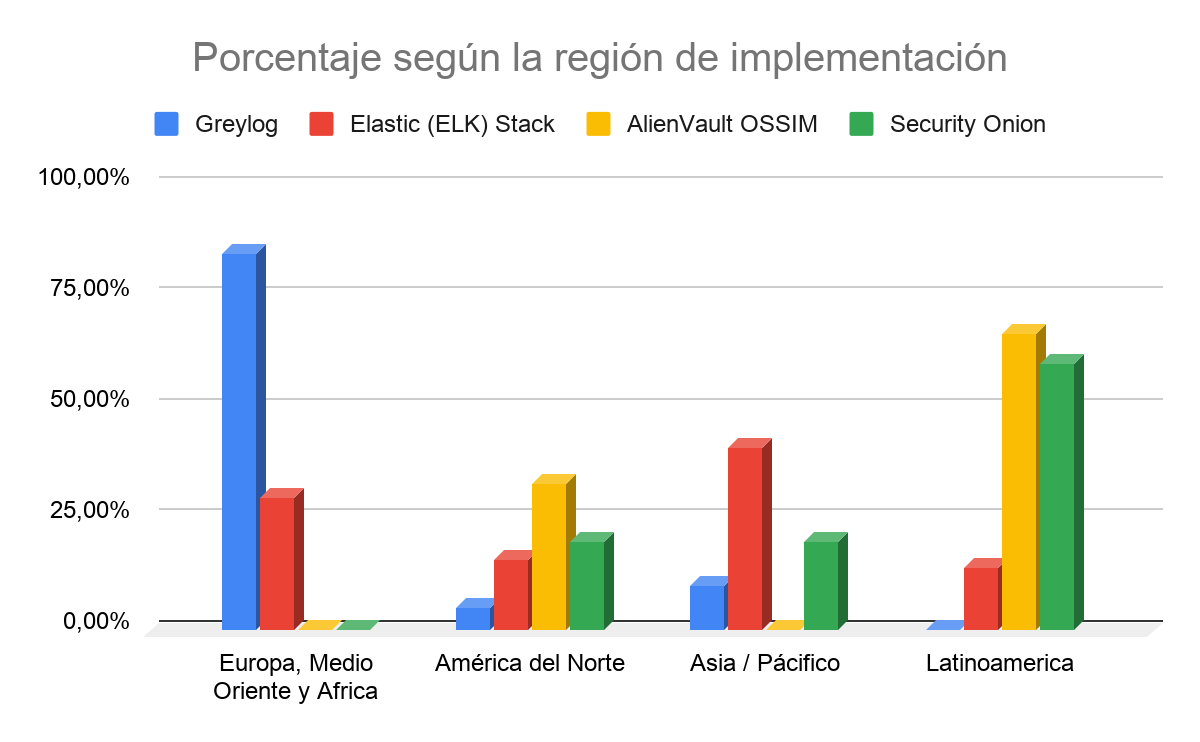
\includegraphics[width=1\textwidth]{./marco_teorico_imagenes/figura_14_region_implen_sol_libre.png}
            \caption{Porcentaje según la región de implementación}
            \label{fig:region_implen_sol_libre}
        \end{figure}
        
        Otra conclusión que se puede destacar del gráfico es que en América del norte y del sur la solución SIEM más utilizada es AlienVault OSSIM \cite{alienvault_ossim}, mientras que en Europa, Medio Oriente y África es Graylog \cite{graylog} así como en Asia/Pacífico optan por la pila Elastic\cite{elastic}.\par
        
            \begin{subsubsection}{AlienVault OSSIM}
            AlienVault OSSIM \cite{alienvault_ossim} es una solución desarrollada por la compañía estadounidense de telecomunicaciones AT \& T. Se trata de una alternativa libre a AlienVault USM, que es la solución comercializada por la empresa. Permite la recopilación, normalización y correlación de eventos, ofreciendo un subconjunto de las capacidades de la variante comercial. El fabricante recomienda esta solución para profesionales IT de organizaciones pequeñas y de pocos recursos, investigadores de seguridad y miembros de la comunidad académica. \par
            Sus capacidades de monitoreo incluyen entornos físicos y virtuales pero no permite un despliegue descentralizado, ya que solo admite la instalación en un único servidor. Entre sus limitaciones se cuentan la ausencia de gestión de logs y la capacidad de detección en puntos finales. A pesar de esto, es la solución SIEM más utilizada en América Latina.

            \end{subsubsection}
            \begin{subsubsection}{Graylog}
            Graylog \cite{graylog} es una solución SIEM desarrollada por la compañía del mismo nombre. Dispone de una arquitectura enfocada a la administración centralizada de logs y, a diferencia de otros sistemas, es capaz de recibir y procesar datos en distintos formatos tales como Syslog, NetFlow, JSON, entre otros. Permite una arquitectura de despliegue descentralizada, donde la recolección, normalización y correlación de eventos se llevan a cabo de manera centralizada. Utiliza una base de datos de elasticsearch y es una solución apta para escalar al tamaño que requiera cualquier organización. \par 
            Entre sus principales ventajas se encuentra su motor de procesamiento de logs, que permite consultar y procesar información de una manera más eficiente que otras soluciones disponibles. Otra de sus ventajas es la tolerancia a fallos, que previene la pérdida de datos en el caso de producirse algún problema de red. Esto facilita el almacenamiento distribuido de datos y el balanceo de carga en las bases de datos. Como se observa en la Figura \ref{fig:region_implen_sol_libre}, Graylog es la solución SIEM más utilizada en Europa, Medio Oriente y África.

            \end{subsubsection}
            \begin{subsubsection}{Elastic Stack}
            Elastic Stack\cite{elastic}, a diferencia de las soluciones descritas anteriormente, no constituye por sí mismo un SIEM como plataforma integral. Sin embargo, es utilizado como columna vertebral de muchos proyectos de software libre, código propietario y soluciones a medida debido a su capacidad de procesamiento de la información. \par
        	Elastic Stack se destaca por el soporte de mensajes provenientes de múltiples fuentes y despliegue de distintos tipos de arquitecturas. Como resultado, dispone de capacidades de almacenamiento tales como escalamiento de infraestructuras, alta disponibilidad, recuperación automática de réplicas y balanceo de carga, etc. En cuanto a la visualización cuenta con una GUI web que permite definir consultas e interactuar con los datos recibidos, mostrando los resultados de una manera intuitiva y visible. 

            \end{subsubsection}
            \begin{subsubsection}{Security Onion}
            Se trata de una distribución Linux basada en Ubuntu \cite{ubuntu} que cuenta con un suite de diversas herramientas dedicadas a la ciberseguridad. Utiliza la pila completa de Elastic Stack para la recopilación, procesamiento y visualización de la información. Admite distintos tipos de arquitectura de despliegue, permitiendo adaptar los recursos disponibles según las necesidades de una organización. Actualmente se encuentra en desarrollo y cuenta con el soporte activo de una comunidad. Es la solución elegida para el desarrollo de este proyecto integrador.
            \end{subsubsection}
            
        \end{subsection} 
    \end{section}
    \begin{section}{Corolario}
    El uso masivo de las tecnologías de la información, así como la convergencia e interconexión de redes y sistemas, ha generado nuevos tipos de riesgos y amenazas en las organizaciones. Los ataques han evolucionado en complejidad, sigilo y focalización de los objetivos, implicando de esta manera mayores esfuerzos para su detección y resolución. \par
	Las organizaciones, públicas y privadas, deben esforzarse en preservar la seguridad de sus activos de información y responder a los nuevos riesgos e incidentes. Esto lleva a la necesidad de desplegar soluciones del tipo CSIRT. \par
    La Universidad Nacional de Córdoba, por sus características como organización y teniendo en cuenta el panorama anteriormente descrito, no se encuentra exceptuada de posibles ciberataques contra sus activos de información. Por lo tanto, se encuentra justificada la creación de un CSIRT que atienda a sus propias necesidades. \par

    \end{section}
            
            
            
            

    \chapter{Descripción de Requerimientos}
    Con el objetivo de desplegar un sistema SIEM capaz de soportar los requerimientos funcionales y no funcionales, es necesario definir el entorno en el que operará la plataforma. \par
    Para esto se requiere, en primer lugar describir la topología de la red de la organización, es decir realizar un relevamiento de las conexiones  de la infraestructura de red interna del área central, de sus dependencias y la red entre las unidades geográficamente distribuidas si las hubiera. Debe incluirse la topología de las conexiones de salida a Internet. \par
    %En segundo lugar será necesario inventariar los activos de la organización: se requerirá una investigación y un relevamiento de los activos con los que cuentan las infraestructuras de red y de datos a fin de clasificarlos. \par
    Las tareas de relevamiento anteriormente descritas proporcionarán un entendimiento acabado y profundo de la situación en la que se encuentra la infraestructura. Como resultado, será posible identificar puntos críticos a tener en consideración y como consecuencia, elegir la solución que mejor se ajuste a las necesidades de la organización. \par

    \begin{section}{Requerimientos funcionales del SIEM}
    A continuación se listan los requerimientos funcionales:
    \begin{enumerate}
        \item Recolectar y almacenar datos de incidentes de seguridad en la infraestructura de la red corporativa.
        \item Recolectar y almacenar información contextual y asociada a los activos vinculados  al incidente.
        \item Visualizar las alertas en un tablero de mando. 
        \item Implementar un sistema de envío de alertas de seguridad que notifique a los responsables de activos de información afectados.
        \item Definir un criterio para priorizar alertas.
        \item Implementar un sistema de correlación de alertas de seguridad.
    \end{enumerate}
        
    \end{section}
    \pagebreak
    \begin{section}{Requerimientos no funcionales}
    A continuación se listan los requerimientos no funcionales:
    \begin{enumerate}
        \item La solución propuesta debe utilizar software libre.
        \item La solución debe ser compatible con sistemas operativos abiertos y de tipo Unix. 
        \item La arquitectura de la solución debe ser escalable a demanda de la organización.
        \item Se requiere un despliegue automatizado de la solución.
    \end{enumerate}

    \end{section}
    \begin{section}{Análisis de riesgo}
    A partir de la definición de los requerimientos, se procedió a realizar un análisis de riesgo en el que se evaluaron las distintas soluciones SIEM mencionadas en el Marco Teórico. El objetivo de esta comparación fue encontrar la solución que mejor se adaptase los requerimientos formulados. \par
    En primer lugar, se codificaron los requerimientos funcionales y no funcionales en el Cuadro \ref{table:6}, así como las soluciones disponibles en el Cuadro \ref{table:7}. Esta codificación fue utilizada para comparar las soluciones contra los requerimientos del proyecto, para obtener una apreciación general de la viabilidad de cada solución, en términos de su potencial elección para el desarrollo del proyecto. Los Cuadros \ref{table:6} y \ref{table:7} se presentan a continuación:
    \begin{table}[H]
        \centering
        \begin{tabular}{|m{4em}|m{30em}|}
        
            \hline 
                Siglas  & Requerimientos \\ 
            \hline
                RF1 & Recolectar y almacenar datos de incidentes de seguridad en la infraestructura de la red corporativa. \\ 
            \hline
                RF2  & Recolectar y almacenar información contextual y asociada a los activos vinculados al incidente. \\ 
            \hline
                RF3 & Visualizar las alertas en un tablero de mando. \\
            \hline
                RF4 & Implementar un sistema de envío de alertas de seguridad que notifique a los responsables de activos de información afectados. \\
            \hline
                RF5 & Definir un criterio para priorizar alertas. \\
            \hline
                RF6 & Implementar un sistema de correlación de alertas de seguridad.. \\
            \hline
                RNF1 & La solución propuesta debe utilizar software libre. \\
            \hline
                RNF2 & La solución debe ser compatible con sistemas operativos abiertos y de tipo Unix. \\
            \hline
                RNF3 & La arquitectura de la solución debe ser escalable a demanda de la organización. \\
            \hline
                RNF4 & Se requiere un despliegue automatizado de la solución. \\
            \hline %linea final de tabla
        \end{tabular}
        \caption{Codificación de requerimientos funcionales y no funcionales.}
        \label{table:6}
    \end{table}
     %\FloatBarrier
    \begin{table}[H]
        \centering
        \begin{tabular}{|m{6em}|m{20em}|}
        
            \hline 
                Siglas  & Solución \\ 
            \hline
                S1 & Graylog \\ 
            \hline
                S2  & Elastic (ELK) Stack \\ 
            \hline
                S3 & AlienVault OSSIM \\
            \hline
                S4 & Security Onion \\
            \hline
                S5 & Splunk. \\
            \hline
                S6 & McAfee Enterprise Security Manager \\
            \hline
                S7 & AlienVault USM \\
            \hline
                S8 & QRadar SIEM \\
            \hline
                S9 & ManageEngine ADAudit Plus \\
            \hline
                S10 & LogRhythm NextGen SIEM Platform \\
            \hline
                S11 & LogPoint - SIEM \\
            \hline
                S12 & ArcSight Enterprise Security Manager (ESM) \\
            \hline
                S13 & InsightIDR \\
            \hline %linea final de tabla
        \end{tabular}
        \caption{Codificación de las soluciones disponibles.}
        \label{table:7}
    \end{table}
     \FloatBarrier
     
     Posteriormente, se priorizaron los requerimientos funcionales y no funcionales. Se eligieron tres categorías: Alta, Media y Baja. A continuación se describen detalladamente estos niveles.\par
     Los requerimientos funcionales definidos como de “Alta” prioridad son los que se consideraron que no pueden faltar en una solución SIEM, ya que son inherentes a la naturaleza del mismo. Por otro lado los requerimientos no funcionales de la misma categoría plantean una restricción que no se puede evitar. El incumplimiento de por lo menos uno de estos requerimientos, llevó a descartar la solución. \par
     El nivel de prioridad “Media” para los requerimientos implica  que el cumplimiento de estos es deseable para hacer mejor uso de la solución, pero no impactan significativamente en el desempeño general si no son implementados.\par
     Por último, un nivel de prioridad “Baja” implica que los requerimientos de este tipo están orientados a optimizar la solución, una vez que está ya se encuentre funcionando. Su incumplimiento no es crítico. \par 
     La información resultante se muestra en el Cuadro \ref{table:8}.
     \begin{table}[H]
        \centering
        \begin{tabular}{|m{3em}|m{28em}|m{4em}|}
        
            \hline 
                Siglas & Requerimientos & Prioridad \\ 
            \hline
                RF1 & Recolectar y almacenar datos de incidentes de seguridad en la infraestructura de la red corporativa. & Alta \\ 
            \hline
                RF2  & Recolectar y almacenar información contextual y asociada a los activos vinculados al incidente. & Media\\ 
            \hline
                RF3 & Visualizar las alertas en un tablero de mando. & Alta\\
            \hline
                RF4 & Implementar un sistema de envío de alertas de seguridad que notifique a los responsables de activos de información afectados. & Media \\
            \hline
                RF5 & Definir un criterio para priorizar alertas. & Baja\\
            \hline
                RF6 & Implementar un sistema de correlación de alertas de seguridad. & Media \\
            \hline
                RNF1 & La solución propuesta debe utilizar software libre. & Alta\\
            \hline
                RNF2 & La solución debe ser compatible con sistemas operativos abiertos y de tipo Unix. & Alta \\
            \hline
                RNF3 & La arquitectura de la solución debe ser escalable a demanda de la organización. & Media \\
            \hline
                RNF4 & Se requiere un despliegue automatizado de la solución. & Baja\\
            \hline %linea final de tabla
        \end{tabular}
        \caption{Valoración de requerimientos funcionales y no funcionales.}
        \label{table:8}
    \end{table}
     \FloatBarrier
     En el Cuadro \ref{table:9} se muestran todas las soluciones disponibles y cuales son los requerimientos que cumplen. Este cuadro fue elaborado con las codificaciones extraídas de los Cuadros \ref{table:6} y \ref{table:7}. El resultado permitió valorar la viabilidad de cada solución en términos de cumplimiento de requerimientos y contribuyó a una preselección inicial de soluciones. 
     \begin{table}[H]
        \centering
        \begin{tabular}{|m{4em}|m{2em}|m{2em}|m{2em}|m{2em}|m{2em}|m{2em}|m{3em}|m{3em}|m{3em}|m{3em}|}
        
            \hline 
                Solución & RF1& RF2& RF3& RF4& RF5& RF6& RNF1& RNF2& RNF3& RNF4 \\ 
            \hline
                S1 & Sí & Sí & Sí & Sí & Sí & Sí & Sí & Sí & Sí & Sí \\ 
            \hline
                S2  & Sí & Sí & Sí & Sí & No & Sí & Sí & Sí & Sí & Sí   \\ 
            \hline
                S3 & Sí & No & Sí & No & No & Sí & Sí & Sí & No & Sí   \\
            \hline
                S4 & Sí & Sí & Sí & Sí & Sí & Sí & Sí & Sí & Sí & Sí  \\
            \hline
                S5 & Sí & Sí & Sí & Sí & Sí & Sí & No & Sí & Sí & Sí  \\
            \hline
                S6 & Sí & Sí & Sí & Sí & Sí & Sí & No & Sí & Sí & Sí \\
            \hline
                S7 & Sí & Sí & Sí & Sí & Sí & Sí & No & Sí & Sí & Sí \\
            \hline
                S8 & Sí & Sí & Sí & Sí & Sí & Sí & No & Sí & Sí & Sí \\
            \hline
                S9 & Sí & Sí & Sí & Sí & Sí & Sí & No & Sí & Sí & Sí \\
            \hline
                S10 & Sí & Sí & Sí & Sí & Sí & Sí & No & Sí & Sí & Sí \\
            \hline
                S11 & Sí & Sí & Sí & Sí & Sí & Sí & No & Sí & Sí & Sí \\
            \hline
                S12 & Sí & Sí & Sí & Sí & Sí & Sí & No & Sí & Sí & Sí \\
            \hline
                S13 & Sí & Sí & Sí & Sí & Sí & Sí & No & Sí & Sí & Sí \\
            \hline %linea final de tabla
        \end{tabular}
        %CENTRAR EL NOMBRE DE ESTE CUADRO 
        \caption{Comparación entre las soluciones disponibles y los requerimientos del proyecto.}
        \label{table:9}
    \end{table} 
     \FloatBarrier
     Considerando al RNF1 como un requerimiento de alta prioridad y fundamental para el desarrollo de este proyecto, se procedió a descartar las soluciones comerciales por más que cumplieran con los demás requerimientos de alta prioridad. Esto llevó a continuar el análisis de riesgos teniendo en cuenta solamente las soluciones gratuitas y de código abierto.\par
    Definidos los niveles de requerimientos de las soluciones, se plantea un sistema de puntuación, donde se asignan valores según la prioridad. El resultado se observa en el Cuadro \ref{table:10}.
    \begin{table}[H]
        \centering
        \begin{tabular}{|m{16em}|m{7em}|}
        
            \hline 
                Tipo de prioridad  & Valoración \\ 
            \hline
                Alta & 3 \\ 
            \hline
                Media  & 2 \\ 
            \hline
                Baja & 1 \\
            \hline %linea final de tabla
        \end{tabular}
        \caption{Valoración de prioridades de los requerimientos}
        \label{table:10}
    \end{table}
     \FloatBarrier
    Se utilizó un sistema de valoración para contrastar las soluciones preseleccionadas y elegir la más adecuada para este proyecto. \par
    El proceso consistió en comparar  los datos sobre el cumplimiento o no de los requerimientos, que fueron extraídos del Cuadro \ref{table:9}. Posteriormente se asignó un puntaje mediante un sistema de valoración. Este último consistió en multiplicar el valor de cada prioridad por uno (1) si el requerimiento era satisfecho por la solución, en caso contrario el valor asignado fue cero (0). Finalmente los valores fueron sumados y se expuso el resultado final en el Cuadro \ref{table:11}.
    \begin{table}[H]
        \centering
        \begin{tabular}{|m{4em}|m{2em}|m{2em}|m{2em}|m{2em}|m{2em}|m{2em}|m{3em}|m{3em}|m{3em}|m{3em}| m{2em}|}
        
            \hline 
                Solución & RF1& RF2& RF3& RF4& RF5& RF6& RNF1& RNF2& RNF3& RNF4 & Total\\ 
            \hline
                S1 & 1x3 & 1x2 & 1x3 & 1x2 & 1x1 & 1x2 & 1x3 & 1x3 & 1x2 & 1x1 & 22\\ 
            \hline
                S2  & 1x3 & 1x2 & 1x3 & 1x2 & 0x1 & 1x2 & 1x3 & 1x3 & 1x2 & 1x1 & 21   \\ 
            \hline
                S3 & 1x3 & 0x2 & 1x3 & 0x2 & 0x1 & 1x2 & 1x3 & 1x3 & 0x2 & 1x1 & 15  \\
            \hline
                S4 & 1x3 & 1x2 & 1x3 & 1x2 & 1x1 & 1x2 & 1x3 & 1x3 & 1x2 & 1x1 & 22 \\
            \hline %linea final de tabla
        \end{tabular}
        \caption{Valoración de las soluciones libres disponibles.}
        \label{table:11}
    \end{table} 
    \FloatBarrier
    Se observó que las soluciones mejor puntuadas fueron S1, S2 y S4, que corresponden a Greylog, Elastic (ELK) Stack y Security Onion respectivamente. \par
    Como Graylog y Security Onion utilizan parte o todos los componentes de Elastic dentro de un entorno ya configurado, se procedió a descartar como posible solución a la pila Elastic Stack (S2). \par
    La selección final se realizó mediante una comparativa entre Security Onion y Graylog. Si bien en el Cuadro \ref{table:11} se pudo apreciar que ambos lograron la misma valoración total, el elegido para llevar a cabo el proyecto fue Security Onion. Esto se debió a las ventajas que presenta por sobre todas las soluciones participantes, de la que se destaca el polimorfismo a nivel de plataforma. Esta última característica permite que Security Onion asuma tanto las funciones propias de un SIEM como las de un sistema IDS. \par
    Este trabajo fue realizado en conjunto con otros dos Proyectos Integradores. Uno de ellos desplegó y configuro de sensores IDS, esto fue motivo suficiente para optar por Security Onion. \par
    \end{section}
    \pagebreak
    \begin{section}{Orden de implementación de requerimientos}
    
    A continuación se presenta el orden de abordaje de los requerimientos, a lo largo de este documento.  \par
    %ACÁ PONER EXPLICACIÓN DE QUE CAPITULO O ITERACIÓN SE VAN A VER LOS REQUERIMIENTOS PLANTEADOS%
    
    \begin{table}[h]
    \begin{tabular}{|m{3em}|m{26em}|m{4em}|m{4em}|}
    \hline
    \multicolumn{1}{|l|}{Orden} & \multicolumn{1}{c|}{Requerimiento}                                                                                            & Prioridad & Código\\ \hline
    1     & La solución propuesta debe utilizar software libre                                                                            & Alta   & RNF1   \\ \hline
    2     & La solución debe ser compatible con sistemas operativos tipo Unix                                                             & Alta  & RNF2   \\ \hline
    3     & Recolectar y almacenar datos de incidentes de seguridad en la infraestructura de la red corporativa                           & Alta   & RF1   \\ \hline
    4     & Visualizar las alertas en un tablero de mando                                                                                 & Alta     & RF3 \\ \hline
    5     & Recolectar y almacenar información contextual y asociada a los activos vinculados al incidente                                & Media & RF2    \\ \hline
    6     & Implementar un sistema de correlación de alertas de seguridad                                                                  & Media     & RF6 \\ \hline
    7     & Implementar un sistema de envíos de alertas de seguridad que notifique a los responsables de activos de información afectados & Media & RF4    \\ \hline
    8     & La arquitectura de la solución debe ser escalable a demanda de la organización                                                & Media & RNF3    \\ \hline
    9     & Definir un criterio para priorizar alertas                                                                                    & Baja   & RF5   \\ \hline
    10    & Se requiere un despliegue automatizado de la solución                                                                         & Baja  & RNF4    \\ \hline
    \end{tabular}
    \caption{Orden de implementación de los requerimientos de proyecto}
    \label{table:13}
    \end{table}
    \FloatBarrier
    Como se observo en el cuadro \ref{table:13}, en primer lugar se abordaron los requerimientos RF1 y RF3 en la Iteración I. A continuación, los requerimientos RF2, RF6 Y RF4 se desarrollaron en la Iteración II. Finalmente, el requerimiento RF5 fue implementado en la Iteración III. \par
    Los requerimientos no funcionales, como se puede inferir, no son tratados en una iteración numerada. Esto se debe a que fueron desarrollados en el Capítulo 4.
    \end{section}
    
    \chapter{\Large Descripción de Security Onion}
    \begin{section}{Security Onion como sistema de gestión de eventos}
    \begin{figure}[H]
        \centering
        
\includegraphics[width=0.7\textwidth]{./descripcion_sonion_imagenes/figura_15_logo_sonion.png}
        \caption{logo de Security Onion\cite{sonion}}
        \label{fig:logo_sonion}
    \end{figure}
        La elección de Security Onion (versión 16.04) como plataforma se justificó en su naturaleza de código abierto y por sus características destacables respecto de otras soluciones libres, como el soporte de una activa comunidad, el desarrollo continuo de mejoras, actualizaciones y correcciones, su capacidad polimórfica y funcional de actuar como IDS, plataforma SIEM o cluster de almacenamiento. Esto permitió desarrollar distintas arquitecturas de una manera fácil y asistida para el despliegue y la consiguiente optimización de los recursos de hardware y de red. \par
        Otras de las propiedades destacables es la capacidad de integración directa con un conjunto casi universal de los sistemas IDS disponibles, tanto libres como propietarios. Security Onion también incluye un paquete de configuraciones iniciales predefinidas para la infraestructura inicial del sistema, tales como el almacenamiento, normalización y gestión de logs, sistemas IDS y de gestión de usuarios, entre otros. \par
    \end{section}
    \begin{section}{Arquitectura del sistema de gestión de eventos}
    \end{section}
    \begin{subsection}{Arquitectura de alto nivel}
    \begin{figure}[H]
        \centering
        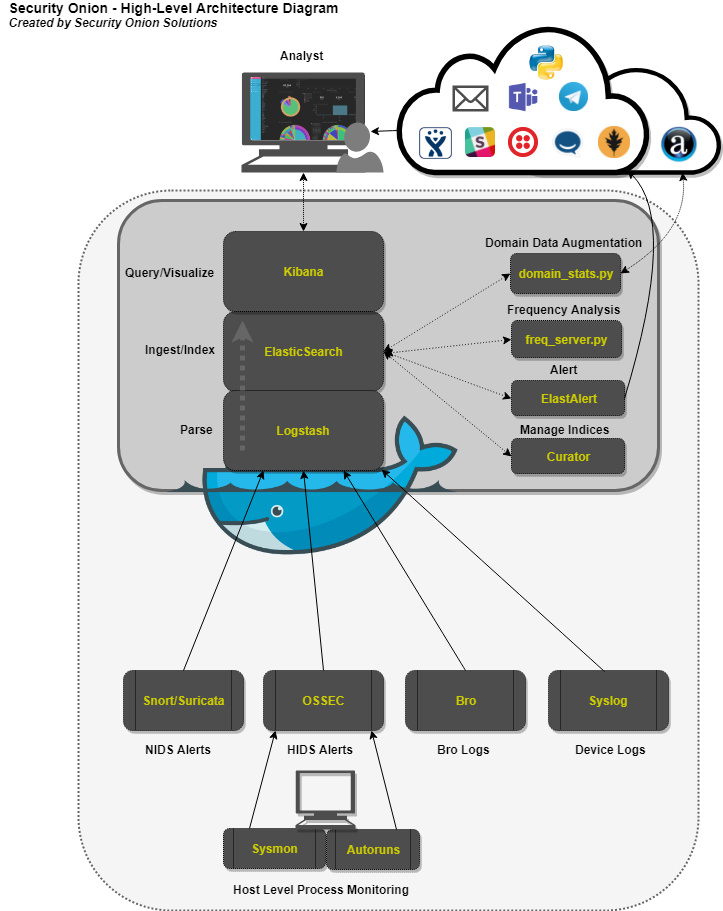
\includegraphics[width=0.7\textwidth]{./descripcion_sonion_imagenes/figura_16_arq_alto_nivel_sonion.png}
        \caption{Security Onion\cite{sonion}: Arquitectura de alto nivel}
        \label{fig:arq_top_sonion}
    \end{figure}
    En la Figura \ref{fig:arq_top_sonion} se observa la distribución de Security Onion y el flujo de datos entre sus componentes principales (la pila Elastic) y secundarios (Curator \cite{curator}, ElastAlert\cite{elasalert}, freqServer\cite{freqserver} y domainStats\cite{domainstat}). Se puede apreciar la conexión con los sistemas de detección IDS como Bro\cite{zeek}, Snort\cite{snort}, Suricata\cite{suricata}, Syslog, etc. Se distinguen también los enlaces con los puntos de administración de los analistas del CSIRT y con los servicios web externos para el envío y recepción de alertas, notificaciones, análisis de tráfico, entre otros. Un punto a destacar es que la pila Elastic se encuentra desplegada en contenedores Docker\cite{docker}. 
    \end{subsection}
    \pagebreak
    \begin{subsubsection}{Tipo de Nodos}
        \begin{itemize}
          \item Nodo Master: este nodo ejecuta su propia copia de la base de datos Elasticsearch, con la que gestiona las búsquedas a través del cluster y estructura a otros nodos en el momento de su despliegue. Lo anterior implica que puede realizar las configuraciones necesarias para los nodos de los tipos “densos” y los de almacenamiento, pero no los de sensores o Forward, por carecer estos últimos de una pila Elastic. Este nodo permite a un analista conectarse mediante un enlace de administración para realizar consultas de los datos.
          \begin{itemize}
              \item  Este nodo contiene los siguientes componentes:
              \begin{itemize}
                  \item Elasticsearch \cite{elastic}
                  \item Logstash \cite{elastic}
                  \item Kibana \cite{elastic}
                  \item Curator \cite{curator}
                  \item ElastAlert \cite{elasalert}
                  \item Redis \cite{redis}
                  \item Wazuh \cite{wazuh} / OSSEC \cite{ossec}
                  \item Sguild \cite{sguil}
              \end{itemize}
          \end{itemize}
          Elasticsearch \cite{elastic}, Kibana \cite{elastic} y Logstash \cite{elastic} son componentes de la pila Elastic, que se tratarán en la siguiente sección junto a ElastAlert \cite{elasalert}. El objetivo de Curator \cite{curator} y Redis \cite{redis} es administrar y optimizar las bases de datos de los nodos de almacenamiento; Wazuh \cite{wazuh} es un IDS y Security Onion lo utiliza para el monitoreo de sí mismo, configurando un sistema HIDS ad hoc, aunque es posible desplegarlo en otros nodos o puntos de interés. Sguild \cite{sguil} permite consultar eventos de una base de datos MySQL desde dentro de Security Onion y muestra los resultados en una GUI. Además, actúa como intermediario de otros componentes secundarios como Squert \cite{squert}, del que detallaremos sus funciones y comportamiento en una sección posterior. 
          \item Nodos Forward: este nodo cumple la función de procesar el tráfico y reenviar los resultados al nodo master. Los logs generados por Snort / Suricata y Bro son enviados mediante syslog a Logstash en el nodo Master, utilizando un túnel ssh, donde finalmente son guardados en la base de datos Elasticsearch, donde pueden ser reenviados a los nodos de almacenamiento. Los logs pueden ser consultados a través de una búsqueda en el cluster.
            \begin{itemize}
               \item Los componentes de un nodo Forward son:
               \begin{itemize}
                   \item Zeek \cite{zeek} (sucesor de Bro)
                   \item Snort \cite{snort} / Suricata \cite{suricata}
                   \item Netsniff-ng \cite{netsniff-ng}
                   \item Wazuh \cite{wazuh} / OSSEC \cite{ossec}
                   \item Syslog-ng \cite{syslog-ng}
               \end{itemize}
            \end{itemize}
            Zeek, Snort / Suricata y Netsniff-ng son procesadores de tráfico (IDS), donde Snort y Suricata serán tratados en una sección posterior. Syslog-ng es utilizado para recolectar logs de los IDS y enviarlos al Logstash del master, donde serán procesados y tratados antes de ser escritos en Elasticsearch.
            \item Nodos Pesados (Heavy Nodes): Es un nodo híbrido entre el nodo Forward y el nodo Master, que incluye todos los componentes del nodo Forward, además de una instancia completa de la pila Elastic. Los nodos pesados envían los resultados de las consultas de su instancia local de Elasticsearch a las solicitudes realizadas por el nodo master mediante un túnel de autossh.
            \begin{itemize}
                \item Los componentes de este nodo son:
                \begin{itemize}
                    \item Elasticsearch
                    \item Logstash
                    \item Curator
                    \item Zeek
                    \item Snort / Suricata
                    \item Netsniff-ng
                    \item Wazuh / OSSEC
                    \item Syslog-ng (envía los logs a la instancia local de Logstash)
                \end{itemize}
            \end{itemize}
            \item Nodos de almacenamiento (Storage Node): su objetivo es extender las capacidades de almacenamiento y procesamiento del nodo Master. Estos nodos despliegan una instancia local de la pila Elastic. De manera análoga a los nodos pesados, cuando se realiza una consulta por parte de la instancia Elasticsearch del nodo Master, esta es procesada por la instancia local del nodo de almacenamiento y devuelta por un túnel autossh.
            \begin{itemize}
                \item Los componentes del nodo de almacenamiento son:
                \begin{itemize}
                    \item Elasticsearch
                    \item Logstash
                    \item Curator
                    \item Wazuh / OSSEC
                \end{itemize}
            \end{itemize}
        \end{itemize}
    \end{subsubsection}
    \pagebreak
    \begin{subsubsection}{Tipos de Arquitectura}
    \label{tipos_de_arquitectura}
      La versatilidad de disponer de múltiples arquitecturas permite adaptar la plataforma a las necesidades de la organización en la que se implante. A continuación, se describen cada una de las opciones posibles:
    \begin{itemize}
         \item Arquitectura monolítica: Consiste en un único servidor que ejecuta simultáneamente los componentes centrales o propios de un nodo Master y los de un nodo sensor. Es un modo híbrido y concentrado que no se recomienda para enlaces de red de alto rendimiento por los elevados requerimientos de hardware necesarios. 
         Este tipo de arquitectura se recomienda para propósitos de pruebas en laboratorio y en entornos de baja demanda de tráfico de red.
        \begin{figure}[H]
            \centering
            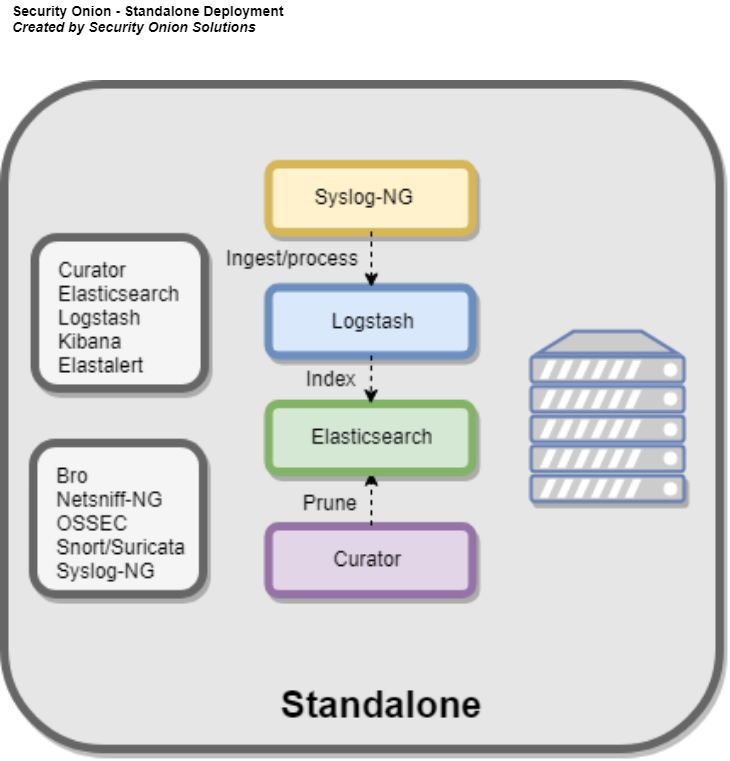
\includegraphics[width=0.7\textwidth]{./descripcion_sonion_imagenes/figura_17_arq_monolitica_sonion.png}
            \caption{Arquitectura monolítica de Security Onion\cite{sonion}}
            \label{fig:arq_monolitica_sonion}
        \end{figure}
        \FloatBarrier
        \pagebreak
        \item Arquitectura densamente distribuida: consiste en uno o más nodos pesados (Heavy Nodes) conectados a un nodo Master. Solo se recomienda en el caso de que no sea posible desplegar una arquitectura distribuida, ya que tiene las mismas deficiencias de rendimiento de la arquitectura monolítica y no es apropiado para entornos de producción y/o enlaces de red de alta velocidad.
        \begin{figure}[H]
            \centering
            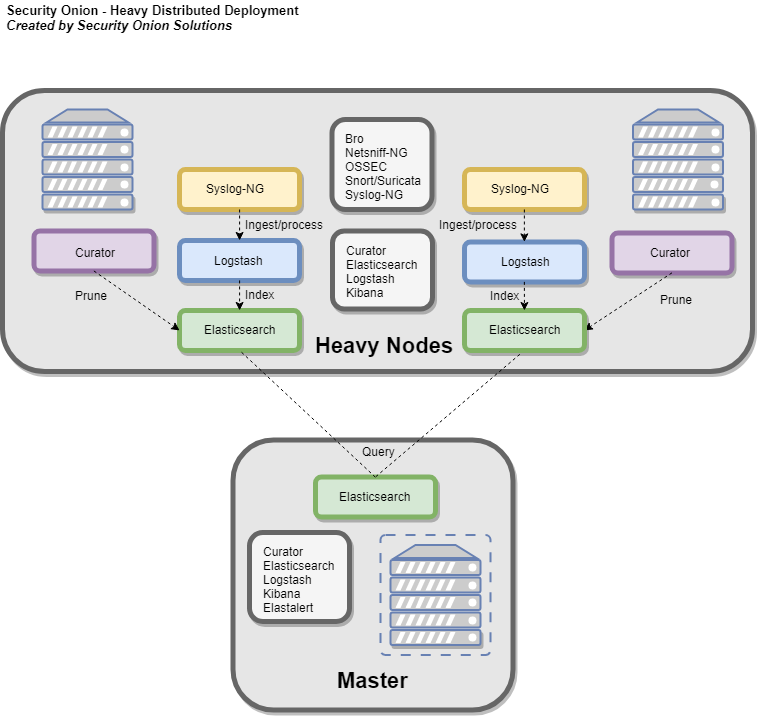
\includegraphics[width=0.7\textwidth]{./descripcion_sonion_imagenes/figura_18_arq_densa_sonion.png}
            \caption{Arquitectura densamente distribuida de Security Onion\cite{sonion}}
            \label{fig:arq_densa_sonion}
        \end{figure}
        \FloatBarrier
        \pagebreak
        \item Arquitectura Distribuida: consiste en un servidor Master, uno o más nodos Forward y uno o más nodos de almacenamiento (Storage Nodes). Es el tipo de despliegue recomendado en términos de eficiencia de requerimientos de hardware, balance de la carga y almacenamiento de datos y optimización general de los recursos disponibles en la organización. 
        \begin{figure}[H]
            \centering
            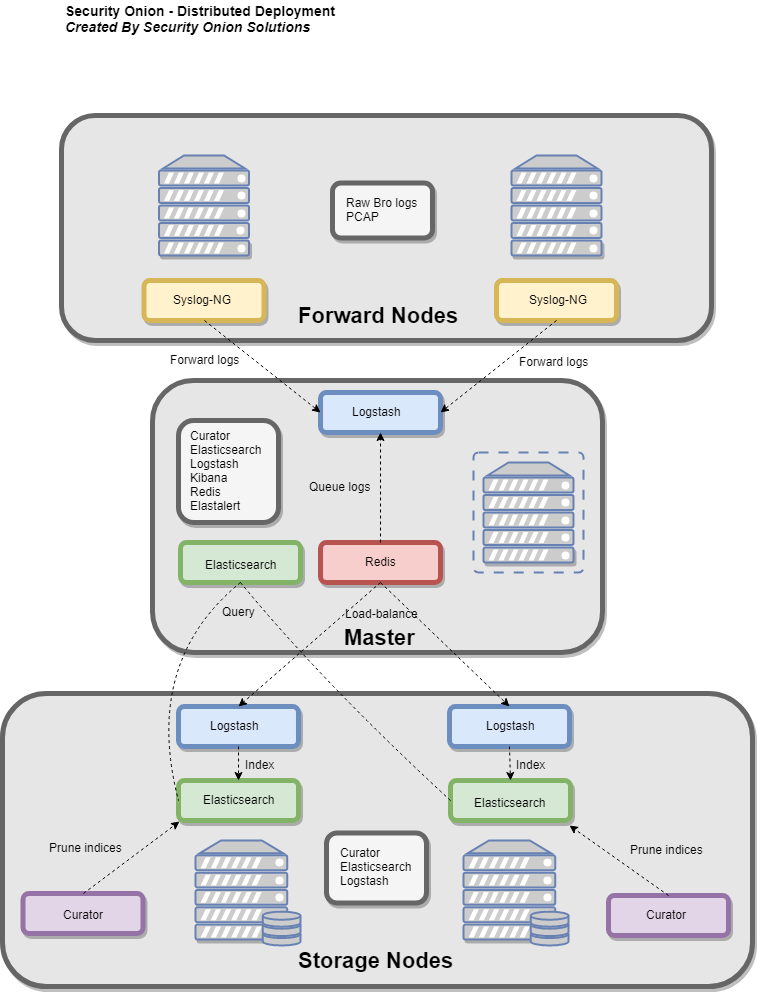
\includegraphics[width=0.7\textwidth]{./descripcion_sonion_imagenes/figura_19_arq_distribuida_sonion.png}
            \caption{Arquitectura distribuida de Security Onion\cite{sonion}}
            \label{fig:arq_distribuida_sonion}
        \end{figure}
     \end{itemize}
   \end{subsubsection}
   \pagebreak
  
   \begin{section}{Recibiendo, procesando y visualizando eventos: La pila Elastic}
   En la Figura \ref{fig:figura_20_conexion_comp_elastic} se observa, que luego de recolectar los datos provenientes de múltiples fuentes, es necesario normalizarlos y agregarlos a la base de datos; estas tareas son llevadas a cabo por los componentes de la pila Elastic (versión 6.8.0), en este caso Logstash y Elasticsearch, respectivamente. 

   \begin{figure}[H]
        \centering
        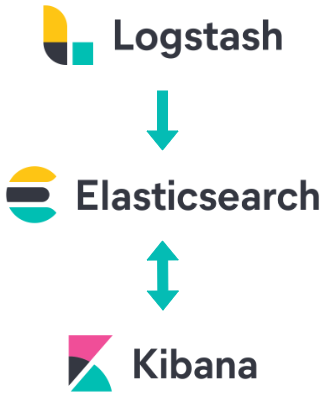
\includegraphics[width=0.45\textwidth]{./descripcion_sonion_imagenes/figura_20_conexion_comp_elastic.png}
        \caption{Conexión de componentes Elastic}
        \label{fig:figura_20_conexion_comp_elastic}
    \end{figure}
        
   \end{section}
   %\pagebreak
   \begin{subsection}{Logstash}
        Logstash es una tubería (en adelante “pipeline”) de procesamiento de datos del lado del servidor que ingesta datos de una multitud de fuentes, los transforma y luego los envía a su destino. Las fuentes de entrada admitidas por logstash son extremadamente amplias, como por ejemplo: syslog, STDIN, TCP, UDP, SNMP, IMAP, entre otras. Posteriormente, Logstash toma los datos sin estructura y los normaliza para crear conjunto ordenado mediante la identificación y conversión de la información a un formato común. Para realizar la tarea anterior, dispone de una gran variedad de filtros que facilitan el procesamiento general, independientemente de la fuente de datos. En este proyecto se utilizó el plugin grok (versión 4.0.4) \cite{grok} como filtro de las fuentes de información. Con los datos ya normalizados, es posible darles un formato específico para un destino en particular, ya que Logstash admite múltiples destinos para la etapa final del pipeline; desde una base de datos, archivos finales o servicios web. Security Onion, por defecto, almacena estos datos normalizados en un formato JSON en la misma pila Elastic, es decir la base de datos Elasticsearch.
   \end{subsection}
   
   \begin{subsection}{Elasticsearch}
        Elasticsearch es una base de datos del tipo NoSQL distribuida y orientada al almacenamiento de documentos. Los datos normalizados provenientes de Logstash son documentos almacenados en índices en Elasticsearch. Cada índice está compuesto por uno o más shards (fragmento), por lo tanto un shard es un subconjunto de documentos, siendo el elemento básico de Elasticsearch y el que permite la escalabilidad del mismo. Un shard es también una instancia de un “índice de Lucene \cite{lucene}", que indexa y almacena un documento en un segmento. Lucene es una librería desarrollada en Java (versión 8) para hacer búsquedas en una base de datos, constituyéndose en un motor de búsqueda que indexa y administra consultas en un conjunto de segmentos. La Figura \ref{fig:figura_21_arq_alm_elasticsearch} muestra la arquitectura de alto nivel del almacenamiento en Elasticsearch.
        
        \begin{figure}[H]
            \centering
            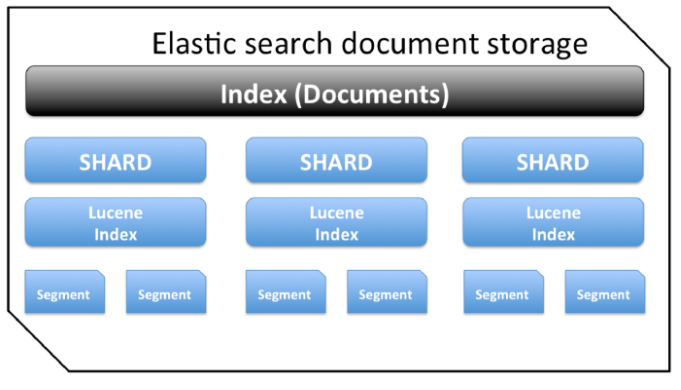
\includegraphics[width=0.7\textwidth]{./descripcion_sonion_imagenes/figura_21_arq_alm_elasticsearch.png}
            \caption{Arquitectura de almacenamiento en Elasticsearch}
            \label{fig:figura_21_arq_alm_elasticsearch}
        \end{figure}
    \end{subsection}
    %\pagebreak
    \begin{subsection}{Kibana}
     Todos los datos almacenados en Elasticsearch pueden ser visualizados por Kibana, una interfaz gráfica perteneciente a la pila Elastic. Kibana permite visualizar los datos en gráficos circulares, de barras, histogramas, etc e interactuar con ellos; también es posible realizar análisis de ubicación cuando se disponen de los metadatos correspondientes mediante el complemento Elastic Maps, realizar análisis de series temporales de una manera rápida y sencilla, dispone de herramientas de inteligencia artificial, que mediante aprendizaje no supervisado permite detectar anomalías y patrones mediante las proyecciones sobre los datos. \par
     Otra de sus características es  la posibilidad de realizar gráficos de correlación y entrecruzamiento, seleccionando campos de interés y filtros lógicos creados por el usuario. Es de destacar que para algunas de estas características es necesario la instalación de plugins complementarios y aunque en su inmensa mayoría son gratuitos, algunos pueden ser pagos ya que utilizan servicios web de la nube de los desarrolladores. 
     \begin{figure}[H]
        \centering
        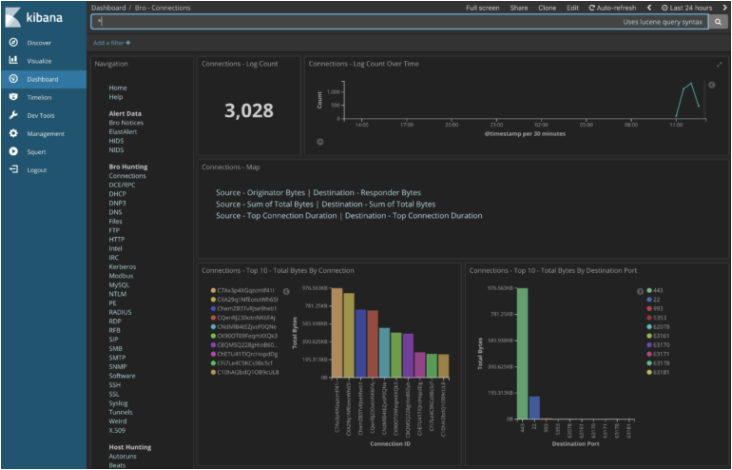
\includegraphics[width=1\textwidth]{./descripcion_sonion_imagenes/figura_22_capt_kibana.png}
        \caption{Captura de pantalla de Kibana\cite{elastic}}
        \label{fig:captura_kibana}
        \end{figure}
   \end{subsection}
   \begin{section}{Elastic, ElastAlert, TheHive y Cortex}
        Security Onion incluye la pila Elastic, cuyos componentes son Logstash quien se encarga de recibir, procesar, normalizar y agregar los datos resultantes a la base de datos  Elasticsearch y Kibana que permite visualizar estos datos. El proceso comienza cuando Logstash recibe los datos sin procesar provenientes de múltiples fuentes, son normalizados por este componente y enviados a Elasticsearch para su almacenamiento. Kibana permite consultar la base de datos mediante una interfaz gráfica de usuario y utilizar esa información para propósitos de análisis de amenazas. \par
        ElastAlert (versión 0.1.39) es un framework que permite identificar y alertar sobre eventos anómalos o patrones de interés sobre los datos de Elasticsearch. También provee múltiples mecanismos para enviar alertas mediante distintas plataformas externas, tales como Slack \cite{slack}, correo electrónico, JIRA \cite{jira}, Telegram \cite{telegram} y muchos más. Tanto ElastAlert como los componentes de la pila Elastic están desplegados sobre contenedores Docker (versión 19.03.12) \cite{docker}. \par
        Es destacable que, aunque Security Onion cubre gran parte de los requerimientos de un SIEM, no posee los elementos que permiten completar un sistema de manejo y respuesta a incidentes; por esta razón y luego de una investigación sobre las alternativas posibles, se incluyó a TheHive (versión 3.3.0) \cite{thehive} y Cortex (3.0.1-1) \cite{thehive} como complemento de Security Onion. TheHive permite la gestión de incidentes de manera detallada y la colaboración con otros CSIRT mediante el uso compartido de información sobre incidentes en tiempo real; mientras que Cortex hace posible la automatización de las respuestas y operaciones ante incidentes utilizando los datos enviados por TheHive. \par

   \end{section}
   \begin{section}{Correlación de eventos: ElastAlert}
   \label{seccion4-5}
     A pesar de que Kibana permite consultar los datos almacenados en Elasticsearch y presentarlos de diversas maneras que resultan en una gran utilidad, carece de la capacidad de generar alertas cuando los datos coinciden con algún patrón, especialmente cuando estos datos son escritos y consultados en tiempo real en la base de datos. Con este objetivo, la plataforma integra a ElastAlert, siendo un componente confiable, modular y simple de configurar. Su funcionamiento se basa en dos componentes principales: reglas y alertas. Las primeras son utilizadas para comparar con los datos resultantes de las consultas que se hacen en forma constante a Elasticsearch, esta comparación consiste en hallar patrones o firmas definidas en las reglas dentro de los datos obtenidos de la consulta; si el resultado de la búsqueda es positivo, una alerta es disparada para notificar el evento. \par
     Las alertas consisten en mensajes que permiten notificar a otro sistema con el objetivo de que este último realice una acción sobre las causas del evento que detectó la regla o bien informar a los analistas y/o responsables definidos. En cualquiera de los dos casos, las alertas pueden incluir toda la información recabada en un formato definido, tales como plantillas o cualquier arreglo configurado a tal fin. \par
     Según la naturaleza de los eventos a clasificar, las reglas cuentan con un conjunto común de paradigmas de monitoreo, estos permiten identificar y generar alertas aprovechando las características de las anomalías al mismo tiempo que optimizan los recursos del resto del CSIRT en términos de hardware y atención de los analistas. Algunos de estos paradigmas se basan en el comportamiento, tales como la frecuencia que consiste en generar una alerta cuando se detectan N cantidad de eventos en un intervalo definido, el cambio de tasas de ocurrencia por arriba o abajo de un límite establecido como normal para un determinado tipo de eventos, cuando en los datos se encuentran presente campos que han sido previamente establecidos como parte de una lista blanca, negra u algún campo cuyo valor coincida con otros tipos de filtros, entre otros. Es posible definir y configurar tantas reglas como alertas sean necesarias. \par

   \end{section}
   \pagebreak
   \begin{section}{El panel de control general: TheHive }
     Como se mencionó en las secciones anteriores, Security Onion requiere de otros elementos capaces de realizar la gestión integral de incidentes y sus respuestas, elementos que sean capaces de condensar y presentar información a los analistas del CSIRT encargados de monitorear y responder a las anomalías e incidentes detectados.  TheHive es la herramienta que se eligió para esta tarea ya que es una plataforma de respuesta a incidentes de seguridad gratuita y de código abierto, cumpliendo así con uno de los requerimientos no funcionales del proyecto, referido al tipo de licencia y accesibilidad al código. Otra de las razones para la elección de esta plataforma en particular ha sido su escalabilidad y su integración con MISP, lo que permite compartir información sobre las amenazas detectadas con otros CSIRT de organizaciones aliadas. Las tres capacidades centrales son la elaboración de casos, la respuesta a estos y la anteriormente mencionada colaboración con otros CSIRT.\par
     \begin{figure}[H]
        \centering
        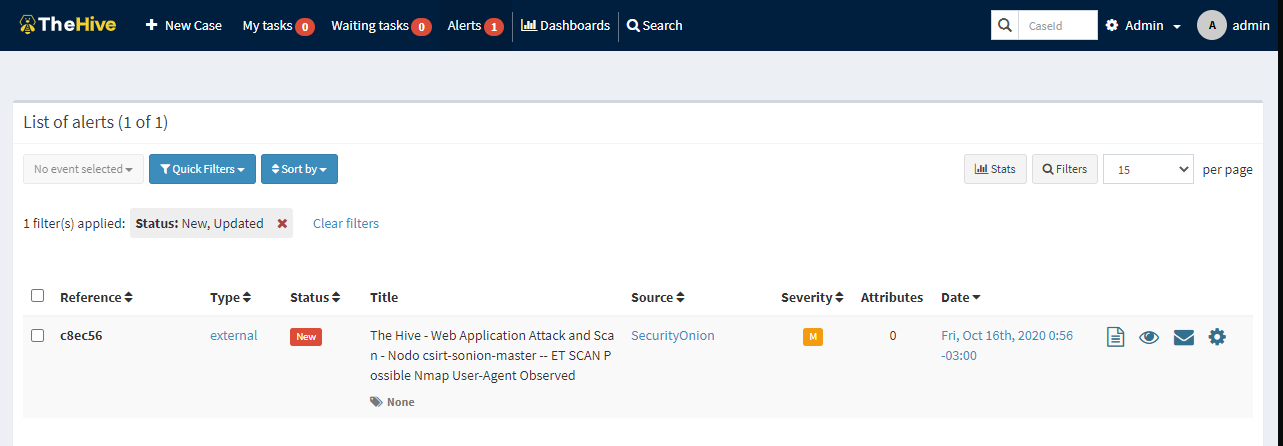
\includegraphics[width=1\textwidth]{./descripcion_sonion_imagenes/figura_23_alerta_panel_thehive.png}
        \caption{ Alertas recibidas en el panel de TheHive\cite{thehive}}
        \label{fig:alerta_panel_thehive}
     \end{figure}
        \FloatBarrier
        En cuanto a la elaboración de casos y tareas asociadas, estas se crean en base a las alertas recibidas \ref{fig:figura_21_arq_alm_elasticsearch}, donde el primer paso consiste en la creación de un caso para luego asociar este a una o varias de las alertas presentes utilizando la plantilla disponible \ref{fig:captura_kibana}, posteriormente es posible agregar tareas asociadas al caso, las cuales se pueden asignar a distintos analistas; a continuación es posible sumar métricas y campos personalizados, reducir el tiempo de búsqueda y recopilación de datos así como automatizar algunas tareas de recopilación de antecedentes en el manejo de incidentes mediante el uso del tablero, tal como se observa en la Figura \ref{fig:alerta_panel_thehive}. En el proceso de creación del caso, TheHive permite agregar cualquier otra información que se considere relevante, como etiquetas, archivos sospechosos de contener malware, etc a modo de evidencias.
        \begin{figure}[H]
        \centering
        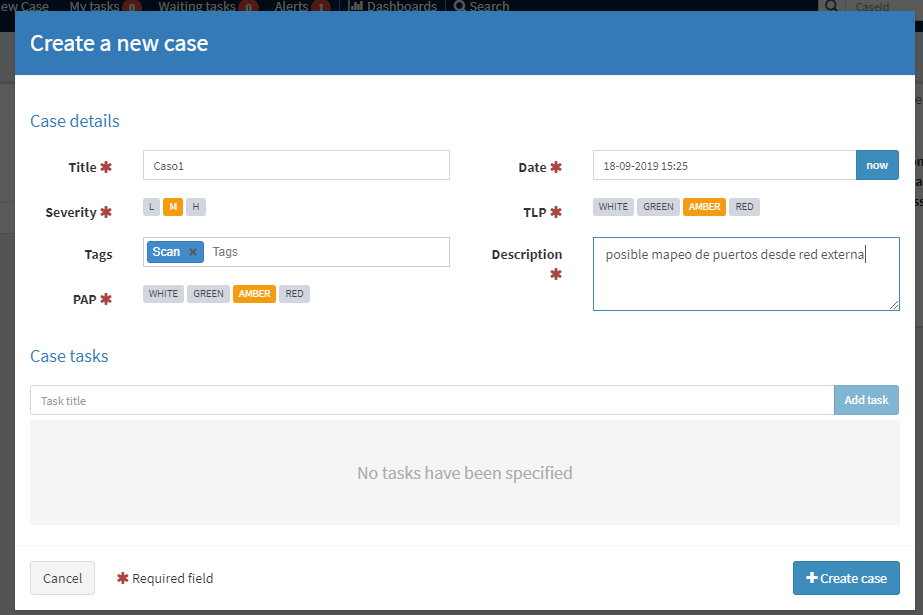
\includegraphics[width=1\textwidth]{./descripcion_sonion_imagenes/figura_24_plantilla_creacion_casos.png}
        \caption{Plantilla para la creación de nuevos casos}
        \label{fig:figura_24_plantilla_nuevos_casos}
     \end{figure}
     \FloatBarrier
     En las figuras \ref{fig:figura_24_plantilla_nuevos_casos} y \ref{fig:dashboard_dinamico} se observan la plantilla de creación de nuevos casos y el tablero que listan los casos existentes, respectivamente.
     \begin{figure}[H]
        \centering
        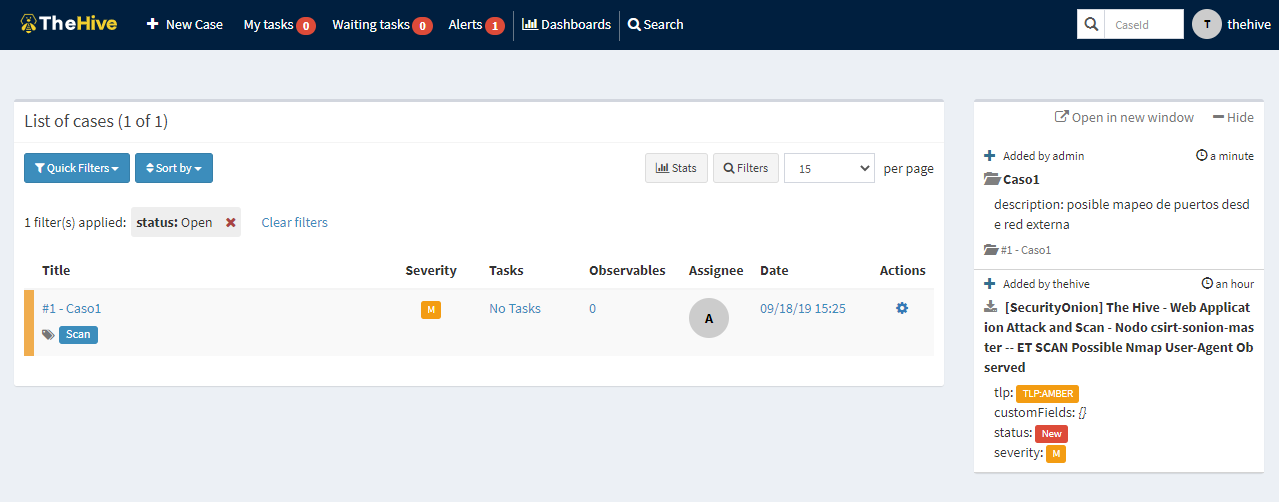
\includegraphics[width=1\textwidth]{./descripcion_sonion_imagenes/figura_25_dashboard_dinamico_thehive.png}
        \caption{Lista de casos de TheHive}
        \label{fig:dashboard_dinamico}
     \end{figure}
     \FloatBarrier
     Luego de la creación de un caso, es posible sumarle todos los “observables” que sean necesarios, donde los observables son todos aquellos campos que se pueden agregar de forma manual y que constituyen fuentes de información para analizar cada caso. Una vez configurado un caso, estos son examinados por scripts llamados “analyzers” que correlacionan y filtran los datos del caso contra los provistos por otras instancias MIPS u otras fuentes de información como la propia base de datos local, servicios de resolución DNS, plataformas como Shodan\cite{shodan}, VirusTotal\cite{virustotal}, Google Cloud Visión\cite{vision-AI}, entre muchas otras. Los observables también se pueden obtener por datos de las alertas recibidas, los cuales son previamente configurados en ElastAlert. Como se mencionó anteriormente ElastAlert realiza consultas a Elasticsearch y con los resultados busca patrones de interés para realizar una notificación, obtenida esta última extrae datos que se consideran de interés para ser enviados a The Hive. Un ejemplo de esto puede ser un número de IP, tipo de protocolo, fecha que se generó el log, puerto de origen y/o destino. La alerta que llega a The Hive contiene todos estos datos, considerados observables. \par
     En la Figura \ref{fig:caso_de_uso_gestion_usuario_conf_thehive} se puede observar los distintos casos de uso para la gestión de usuario que tiene TheHive. Se observa que el administrador puede gestionar usuarios, lo que implica crearlos, bloquearlos o generar API KEYs para ellos. También es posible crear o modificar plantillas de casos y reportes, crear nuevos casos y métricas para estos. Así mismo, existe la posibilidad de  crear Observables, alertas y gestionar estas últimas: TheHive permite ver las alertas recibidas, ejecutar responders y agregar una alerta a un caso existente.\par

     \begin{figure}[H]
        \centering
        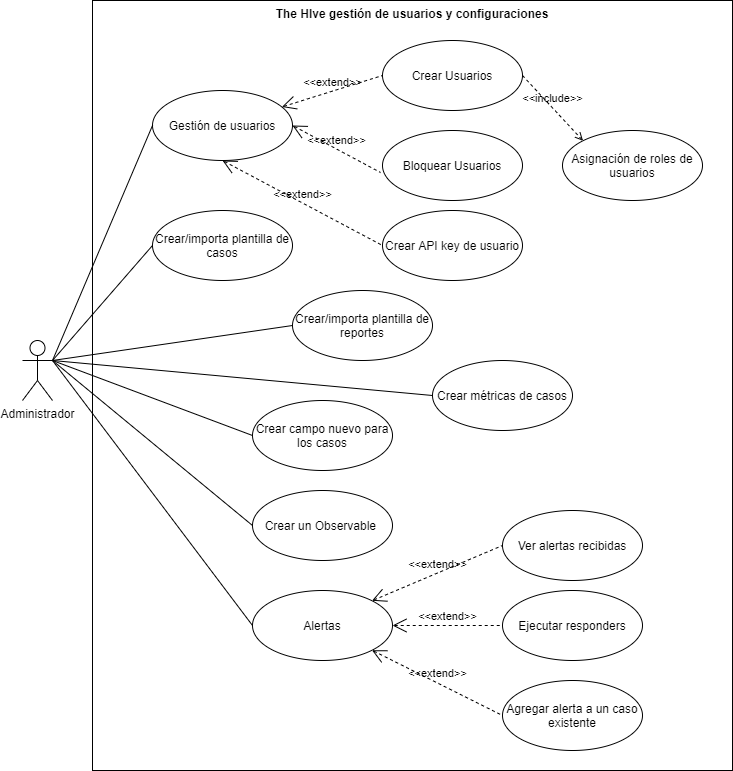
\includegraphics[width=1\textwidth]{./descripcion_sonion_imagenes/figura_28_thehive_user_conf.png}
        \caption{Casos de uso de gestión de usuario y configuraciones de TheHive}
        \label{fig:caso_de_uso_gestion_usuario_conf_thehive}
     \end{figure}
     \FloatBarrier
     En la figura \ref{fig:caso_de_uso_alertas_casos} se muestran las distintas opciones que se le presentan a un usuario de TheHive. Se aprecia que un usuario es capaz de visualizar alertas recibidas, agregar alertas a un caso existente y ejecutar responders de ser necesario. En cuanto a la gestión de casos, un usuario puede ver los casos existentes, crear uno nuevo, eliminar uno existente o unirlo con otro caso, cerrar un caso o en última instancia asignar este último a un usuario diferente. 
     \begin{figure}[H]
        \centering
        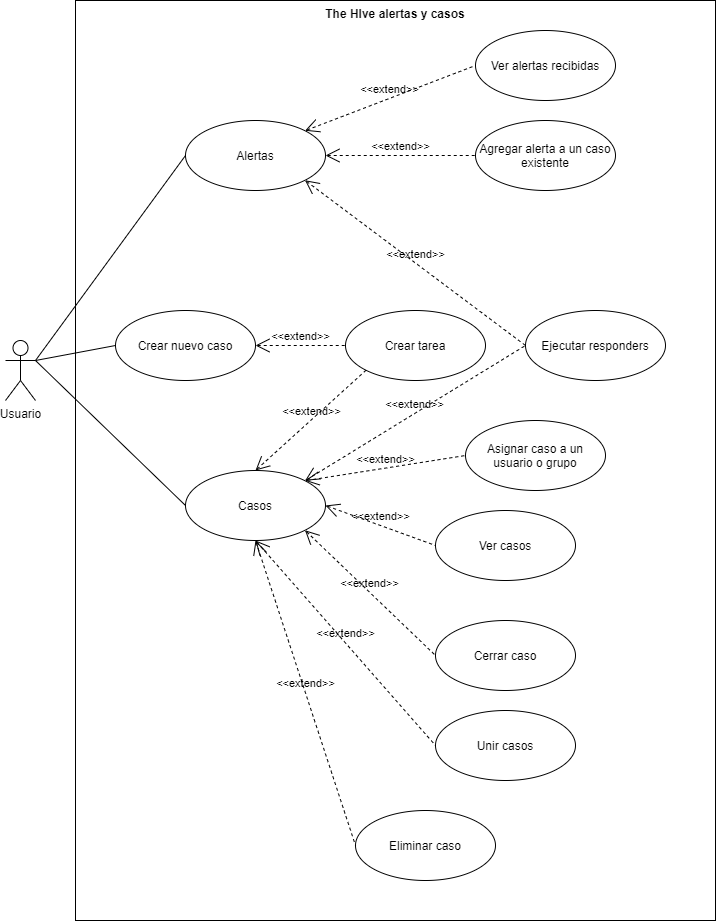
\includegraphics[width=1\textwidth]{./descripcion_sonion_imagenes/figura_29_thehive_alertas_casos.png}
        \caption{Diagrama de casos de uso de alertas y casos}
        \label{fig:caso_de_uso_alertas_casos}
     \end{figure}
     \pagebreak
     \begin{subsection}{Cortex}
        Luego de que el caso fue creado o sobre la misma alerta, el analista puede dar curso a una respuesta mediante “responders” que son scripts en los cuales se encuentra la respuesta del CSIRT a la amenaza. Tanto los responders como los analyzers se encuentran bajo la responsabilidad de Cortex, el subsistema encargado de procesar los casos de TheHive. Al final de esta sección, se presentan los diagramas de casos de uso correspondientes a Cortex.
        En la Figura \ref{fig:analizers_disponibles} se ven los analyzers disponibles. Estos son utilizados por los analistas para contrastar la información disponible con motores de búsqueda especializados como Shodan y VirusTotal. Los responders disponibles se observan en la Figura \ref{fig:ejemplos_responders_cortex}. Los analistas pueden activar o desactivar los mismos desde este panel.
     \begin{figure}[H]
        \centering
        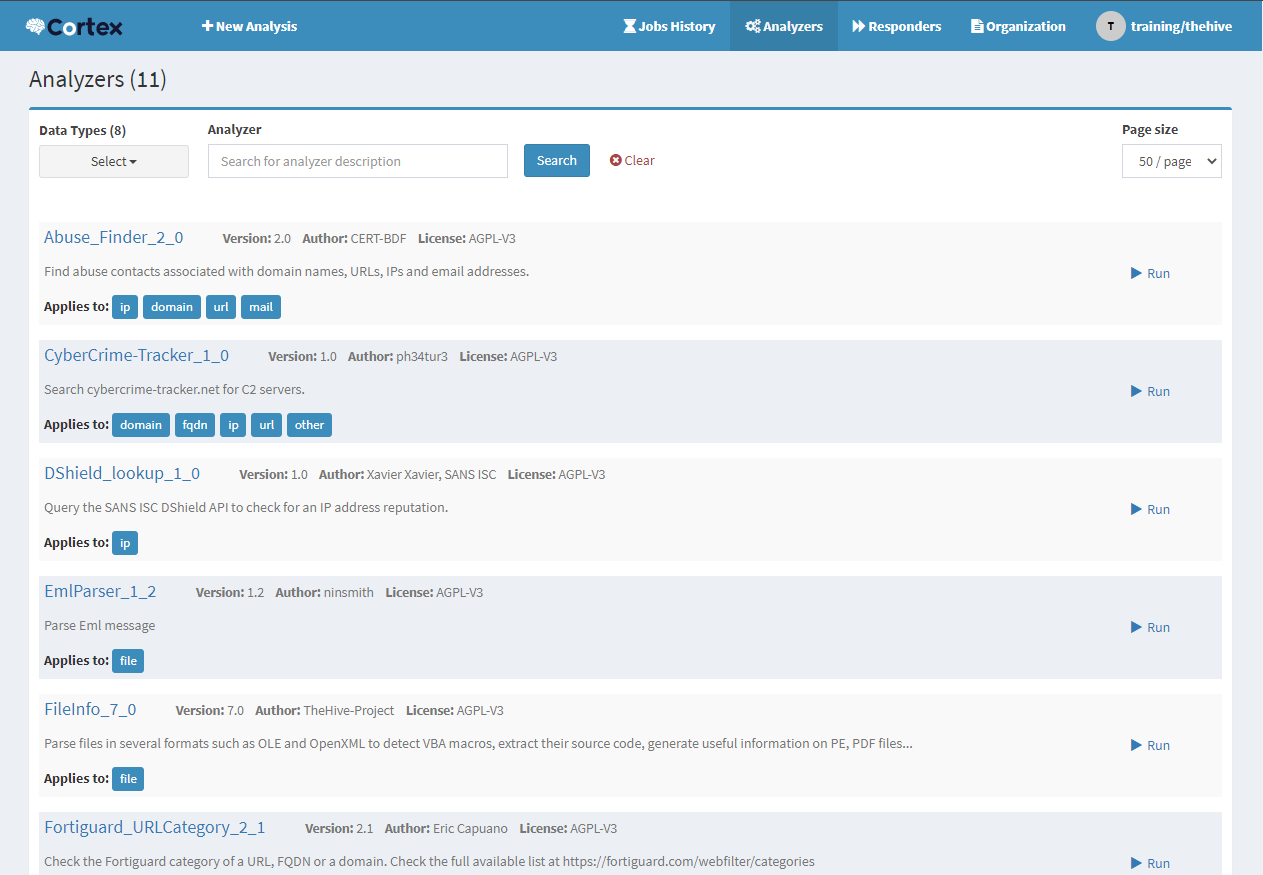
\includegraphics[width=1\textwidth]{./descripcion_sonion_imagenes/figura_26_analyzers_disponibles.png}
        \caption{Algunos de los analyzers disponibles en Cortex}
        \label{fig:analizers_disponibles}
     \end{figure}
     \begin{figure}[H]
        \centering
        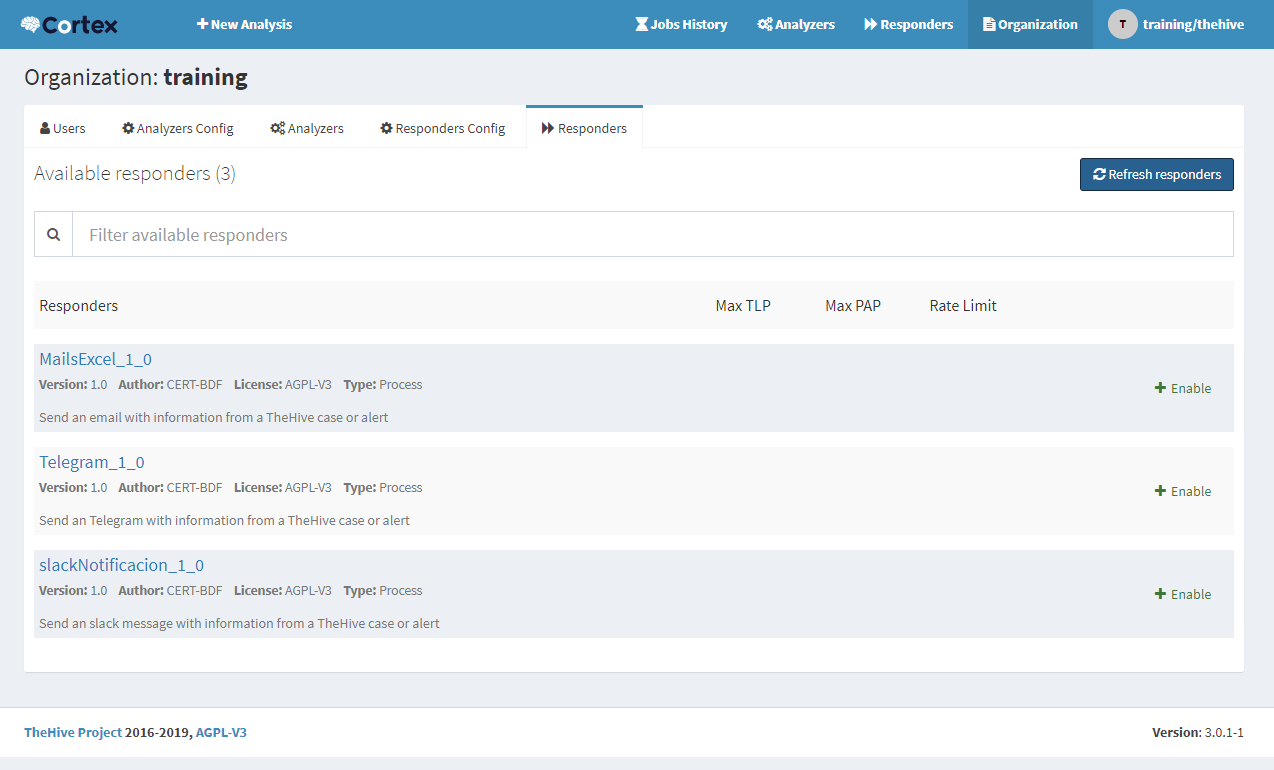
\includegraphics[width=1\textwidth]{./descripcion_sonion_imagenes/figura_27_responders_cortex.png}
        \caption{Ejemplos de responders utilizables en Cortex}
        \label{fig:ejemplos_responders_cortex}
     \end{figure}  
     \FloatBarrier
     En la Figura \ref{fig:caso_de_uso_gestion_usuarios_configuraciones_cortex} se observa el caso de uso de la gestión de usuarios y configuraciones para Cortex. Se muestran las capacidades de gestión tales como crear o bloquear usuarios, crear API KEYs para estos, crear organizaciones y agregarles usuarios a estas. Es posible asignar roles a los usuarios.
     %DIAGRAMA DE CASOS DE USOS DE CORTEX
     \begin{figure}[H]
        \centering
        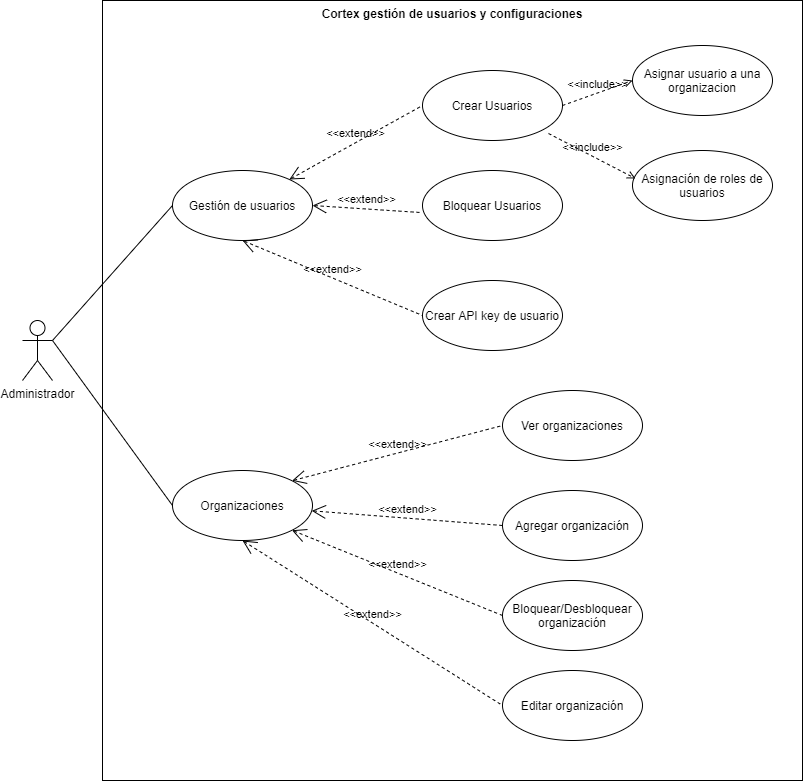
\includegraphics[width=1\textwidth]{./descripcion_sonion_imagenes/figura_30_cortex_user_conf.png}
        \caption{Casos de uso de gestión de usuario y configuraciones de Cortex}
        \label{fig:caso_de_uso_gestion_usuarios_configuraciones_cortex}
     \end{figure}
     \FloatBarrier
     En la Figura \ref{fig:caso_de_uso_tablero_cortex} se observa los casos de usos del panel de Cortex. Las primeras burbujas presentan las pestañas principales del menú de Cortex. El administrador puede crear usuarios de una organización, asignarles roles y permisos, configurar analyzers y responders para una organización.
     \begin{figure}[H]
      \centering
      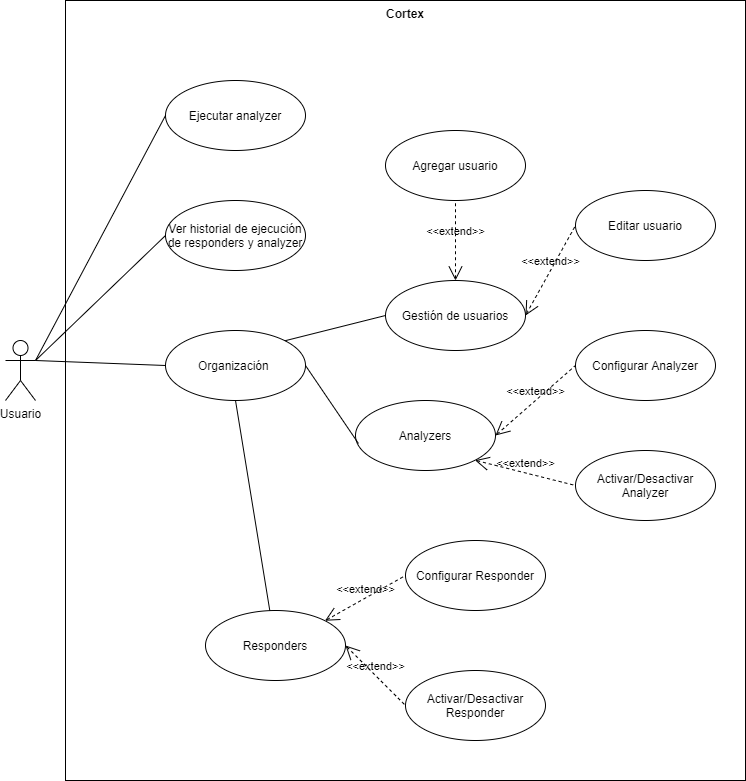
\includegraphics[width=1\textwidth]{./descripcion_sonion_imagenes/figura_31_cortex_tablero.png}
        \caption{Casos de uso del tablero de Cortex}
        \label{fig:caso_de_uso_tablero_cortex}
     \end{figure}
     \end{subsection}
   \end{section}

   \begin{section}{Integración con los sistemas de detección}
        En secciones anteriores se mencionó que Security Onion cuenta con NIDS y HIDS. Durante la configuración inicial del sistema se pueden especificar los NIDS a utilizar, para una configuración rápida de los sensores. Esto permite realizar una primera integración con el hardware disponible. Security Onion cuenta con OSSEC como HIDS para su autodefensa. La implementación de estos sistemas en el SIEM se llevo adelante en otro Proyecto Integrador.
   \end{section}
   \pagebreak
   \begin{subsection}{Suricata, Snort y Ossec}
        Suricata y Snort son motores de detección de amenazas en el tráfico de red. Ambos NIDS se basan en firmas o reglas para realizar la detección de amenazas. Estas firmas son actualizadas constantemente conforme a la aparición de nuevos tipos de ataques, exploits y malware. Si bien estos NIDS son gratuitos y de código abierto, Snort ofrece una versión paga, la cual cuenta con soporte para descargar las firmas actualizadas a la fecha. Por defecto Snort cuenta con las reglas básicas para la detección de amenazas bien conocidas. \par
    	Suricata, por otro lado, es desarrollado y mantenido por los colaboradores de la OISF, los cuales también dan soporte a las firmas ya que se actualizan las existentes y se agregan nuevas en forma permanente. Estas actualizaciones en las reglas son descargadas periódicamente mediante PulledPork, una utilidad que también es usada por Snort cuyo fin es descargar reglas y firmas desde distintos centros de investigación reconocidos en todo el mundo, como el SANS institute, Emerging Threats, entre otros. \par
        En el Cuadro \ref{table:4} se muestran las diferencias entre Snort y Suricata.
        \begin{table}[H]
            \centering
            \begin{tabular}{|m{10em}|m{11em}|m{11em}|}
                \hline 
               \multicolumn{1}{|c|}{Caracteristicas} & \multicolumn{1}{c|}{Snort} & \multicolumn{1}{c|}{Suricata}               \\ \hline % la primera fila se encuentra centrada
                    Desarrollador & CISCO & Open Information Security Foundation (OISF)  \\ 
                \hline
                    Lanzamiento  & 1998 & 2009 \\ 
                \hline
                    Lenguaje del código & C  & C  \\
                \hline
                    Sistema operativo & Linux, Windows y Mac OS X  & Linux, Windows y Mac OS X  \\
                \hline
                    Hilos & Monohilo  & Soporte múltiples hilos  \\
                \hline
                    Soporte IPv6 & Si  & Si  \\
                \hline
                    Reglas de Snort & Si  & Si \\
                \hline
                    Reglas de Emerging Threats & Si  & Si \\
                \hline
                    Formato de logs & unified2  & unified2   \\
                \hline
                    Compatible con Aanval & Si  & Si   \\
                \hline %linea final de tabla
            \end{tabular}
            \caption{Comparación entre Snort y Suricata}
            \label{table:4}
        \end{table}
        \FloatBarrier
        Por otro lado está OSSEC (reemplazado por  Wazuh en las versiones más recientes de Security Onion), es un IDS orientado a hosts (HIDS). Al igual que los NIDS anteriores está basado en firmas para la detección de amenazas, es gratuito y de código abierto. Las reglas pueden descargarse del repositorio disponible en github. \par
   \end{subsection}
   \begin{section}{Corolario del capítulo 4}
        En este capitulo se mostró la solución elegida, sus distintas arquitecturas, sus componentes internos y los subsistemas asociados. Se pudo apreciar a TheHive como una solución complementaria a Security Onion que contribuyo a mejorar la gestión de incidentes.
        En el capítulo siguiente se desarrollo la configuración de un ambiente de prueba y se desplegaron las soluciones mencionadas anteriormente en distintas topologías. Esto permitió dar cumplimiento a los requerimientos funcionales 1 y 3. \par
   \end{section}
    \chapter{\Large Iteración I: “Despliegue e instalación de Security Onion en un ambiente de prueba”}
    En este capítulo describimos la instalación de Security Onion en la topología de red de prueba. Se instalará un nodo \textit{Master}, dos nodos \textit{Forward} y un nodo de \textit{TheHive}. \par
    En este proyecto se trabajó primero sobre un ambiente de prueba y después de producción. En ambos casos se utilizó un servidor central y un sistema operativo de virtualización sobre el que se crearon un conjunto de máquinas virtuales, cada una alojando un servidor con nodos \textit{Forward}, \textit{Master} y el correspondiente a TheHive - Cortex. Se utilizó de guía los componentes, el software y la arquitectura de conexión entre ellos, mencionados en la Descripción de Security Onion. \par
    \begin{section}{Topología de la organización}
    El paso inicial consistió en relevar la topología de la organización, para ello se dispuso de información inicial que fue brindada por los responsables del sector de redes. Posteriormente se realizaron diagramas topológicos con el fin de evaluar la situación y contemplar distintas estrategias para el despliegue de este proyecto.  
    En la Figura \ref{fig:iter1_top_unc} se observa un diagrama que representa la topología de la organización.\par
    Se puede apreciar que las dependencias están conectadas (mediante sus \textit{routers} de borde) entre sí y al mundo exterior mediante el Switch 1 de capa 3 que se encuentra en el \textit{datacenter}. Se observan los servidores 1, 2 y N que representan los activos de información de la organización, éstos están conectados mediante el \textit{Switch} 2 al resto de la organización. Existen M \textit{switches} para otras redes internas del \textit{datacenter}, todos conectados al \textit{Switch} 2. Este \textit{switch}, por lo tanto, conecta las redes internas del \textit{datacenter} y los activos de información con el \textit{Switch} 3, siendo este último el \textit{switch} troncal de la organización. Los enlaces anteriormente mencionados, incluidos los que conectan los \textit{routers} de borde de las dependencias y el \textit{Switch} 3, poseen un ancho de banda de 1 Gbps.\par
    Se observan otros componentes de la infraestructura de la organización, encargados de la conexión exterior con el resto del mundo. Estos son el \textit{Firewall} entre el \textit{Switch} 1 y el \textit{Switch} 5, los \textit{Routers} de borde 1 y 2 junto al \textit{Switch} 6 que se conecta a los proveedores ISP. Todos los enlaces entre estos componentes tienen como característica común un ancho de banda de 10 Gbps. \par
    \begin{figure}[H]
    \centering
    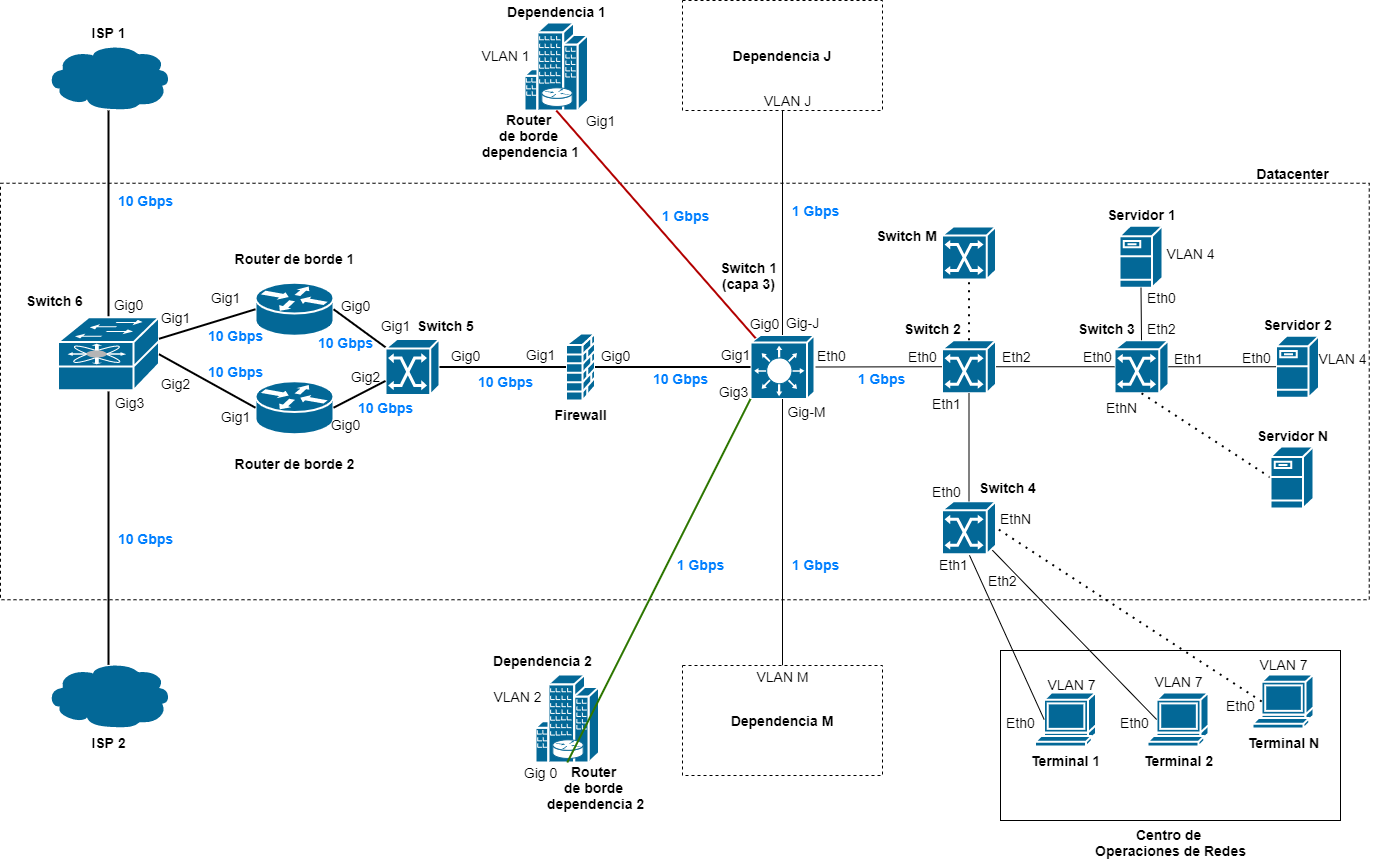
\includegraphics[width=1\textwidth]{./iteracion_1_imagenes/figura_topologia_UNC.png}
    \caption{Topología de la Organización}
    \label{fig:iter1_top_unc}
    \end{figure}
    \FloatBarrier
    \end{section}
    \begin{subsection}{Definición y configuración de las redes a observar}
    Se analizó el ancho de banda de las dependencias existentes y se decidió monitorear dos de ellas. Se seleccionaron las de mayor volumen de tráfico en función de mediciones realizadas a lo largo de una semana y de datos históricos. Las dependencias seleccionadas tenían un enlace con ancho de banda de 1 Gbps cada una. \par
    Las Figuras \ref{fig:figura_35_trafico_dia} muestra el volumen de tráfico medido en un periodo de tiempo de un día (exceptuando las horas en las que la actividad era mínima), mientras que en la Figura \ref{fig:figura_36_trafico_semana} muestra un periodo de una semana. Estos gráficos fueron obtenidos mediante el uso de LibreNMS \cite{librenms} (versión 1.48).\par
    Los datos de las Figuras 5.2 y 5.3 fueron tomados desde la interfaz Gig0 del \textit{Switch} 1 de la Figura 5.1, esto quiere decir que el volumen de tráfico corresponde a la Dependencia1. Las interfaces Gig3, Gig-M y Gig-J del \textit{Switch} 1 tenían un comportamiento similar.\par
    \begin{figure}[H]
    \centering
    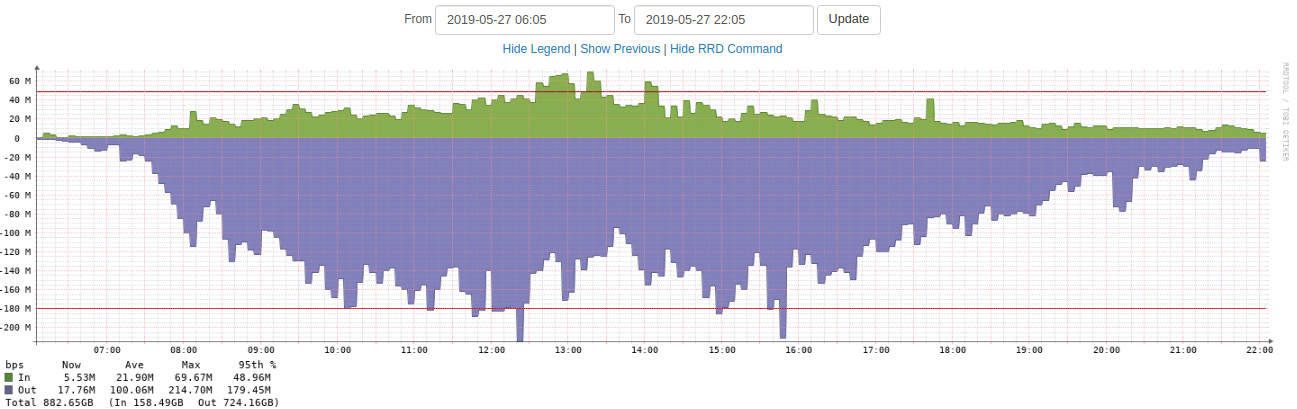
\includegraphics[width=1\textwidth]{./iteracion_1_imagenes/figura_35_trafico_dia.png}
    \caption{Tráfico correspondiente a una dependencia, medido durante un día }
    \label{fig:figura_35_trafico_dia}
    \end{figure}
    \begin{figure}[H]
    \centering
    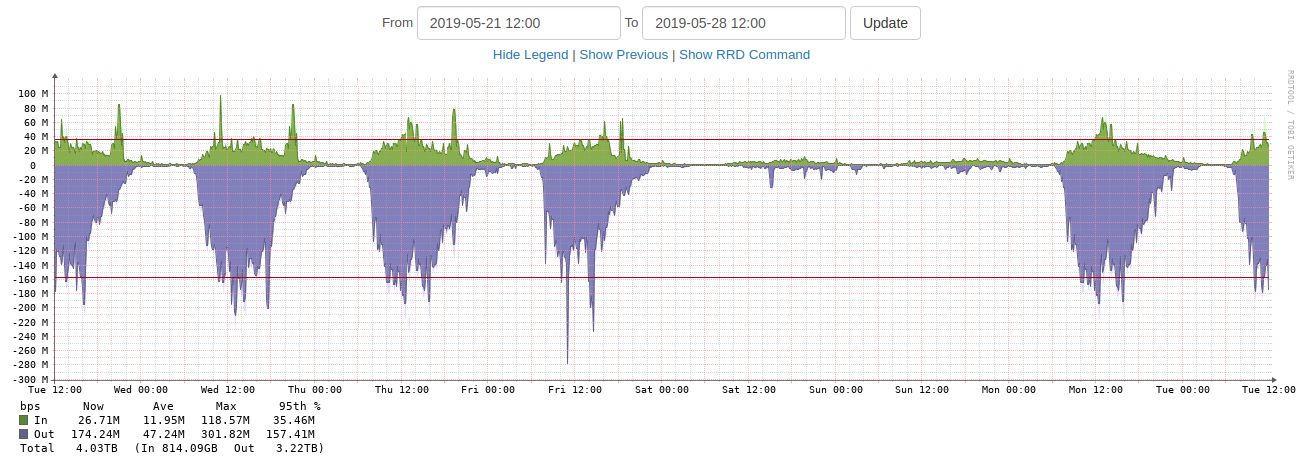
\includegraphics[width=1\textwidth]{./iteracion_1_imagenes/figura_36_trafico_semana_editada.png}
    \caption{Tráfico medido durante el periodo correspondiente a una semana}
    \label{fig:figura_36_trafico_semana}
    \end{figure}
    \FloatBarrier
    En la Figura 5.3 se observa el tráfico de la interfaz Gig0 en el periodo de una semana, donde la velocidad promedio correspondiente a la entrada es de 11,95 Mbps, mientras que de salida es de 47,24 Mbps. Se observaron picos de 300 Mbps de tráfico.\par
    Como la medición corresponde a la interfaz Gig0, el tráfico entrante a esta corresponde al de subida de la Dependencia 1, mientras que el tráfico saliente corresponde al de bajada de esta dependencia.
    \end{subsection}
    \begin{subsection}{Selección de hardware}
    \label{seleccion_hw}
    En primer lugar se examinaron los requisitos de hardware mínimos y recomendados por cada uno de los fabricantes. Para esto se tuvo en cuenta el ancho de banda y el tráfico de los enlaces a monitorear, descritos en la sección precedente. Los requerimientos se presentan a continuación, en los Cuadros \ref{table:15} y \ref{table:5} (para nodos Monolítico y Distribuido, respectivamente). \par
    En base a la Figura \ref{fig:iter1_top_unc}, los datos referidos al tráfico y el ancho de banda de los enlaces a monitorear, se dimensionó el hardware necesario para el servidor central, teniendo en cuenta los requerimientos del fabricante y las limitaciones disponibles en la organización.\par
    %Tabla HW nodo Monolitico
    \begin{table}[H]
    \centering
    \begin{tabular}{|m{10em}|m{10em}|}
    \hline 
    Requerimiento  & Nodo Standalone \\ 
    \hline
    Cantidad de CPU - Arquitectura &  10 nucleos vCPU - x86-64  \\ \hline
    Memoria RAM  &  32 GB  \\ 
    \hline
    Almacenamiento necesario   & 200 GB  \\
    \hline
    Cantidad de interfaces de red  & 2 (administración y monitoreo) \\
    \hline %linea final de tabla
    \end{tabular}
    \caption{Requerimientos de hardware para un nodo Standalone, según el fabricante.}
    \label{table:15}
    \end{table}
     %Tabla HW topología distribuida  
    \begin{table}[H]
    \centering
    \begin{tabular}{|m{9em}|m{9em}|m{9em}|m{9em}|}
    \hline 
    Requerimiento  & Nodo \textit{Master} &  Nodo \textit{Forward} & TheHive y Cortex \\ 
    \hline
    Cantidad de CPU - Arquitectura & Mínimo de 8 núcleos vCPU - x86-64 & Mínimo de 12 núcleos vCPU - x86-64 & Mínimo de 8 núcleos vCPU - x86-64 \\ 
    \hline
    Memoria RAM  & 12 a 128 GB & 128 a 256 GB & A partir de 8 GB \\ 
    \hline
    Almacenamiento necesario & Mínimo de 1 TB  & Mínimo de 540 GB & A partir de 60 GB \\
    \hline
    Cantidad de interfaces de red & 1 (administración) & 2 (administración y monitoreo) & 1 (administración) \\
    \hline %linea final de tabla
    \end{tabular}
    \caption{Requerimientos de hardware recomendados por el fabricante para el monitoreo de un enlace de 1 Gbps}
    \label{table:5}
    \end{table}
    Debido a las restricciones en la disponibilidad del hardware, se realizó una implementación aproximada, teniendo en cuenta los recursos disponibles en la organización. A continuación se muestran los recursos de hardware utilizados, según se trate del despliegue de una topología Monolítica (Cuadro \ref{table:16}) o de una Distribuida (Cuadro \ref{table:12}). \par
    \begin{table}[H]
    \centering
    \begin{tabular}{|m{10em}|m{10em}|}
    \hline 
    Requerimiento  & Nodo Standalone \\ 
    \hline
    Cantidad de CPU - Arquitectura &  4 núcleos vCPU - x86-64  \\ 
    \hline
    Memoria RAM  &  16 GB  \\ 
    \hline
    Almacenamiento necesario   & 500 GB  \\
    \hline
    Cantidad de interfaces de red  & 2 (administración y monitoreo) \\
    \hline %linea final de tabla
    \end{tabular}
    \caption{Requerimientos de hardware utilizados para el despliegue del nodo Standalone.}
    \label{table:16}
   \end{table}
    %En el caso de la topología Distribuida, el hardware que se utilizó para cada nodo se muestra en el Cuadro \ref{table:12}.
    \begin{table}[H]
    \centering
    \begin{tabular}{|m{9em}|m{9em}|m{9em}|m{9em}|}
    \hline 
    Requerimiento  & Nodo \textit{Master} &  Nodo \textit{Forward} & TheHive y Cortex \\ 
    \hline
     Cantidad de CPU - Arquitectura & 8 nucleos vCPU - x86-64 & 10 nucleos vCPU - x86-64 & 8 nucleos vCPU - x86-64 \\ 
    \hline
    Memoria RAM  & 16 GB & 32 GB & 8 GB \\ 
    \hline
    Almacenamiento necesario & 500 GB  & 200 GB & 60 GB \\
    \hline
    Cantidad de interfaces de red & 1 (administración) & 2 (administración y monitoreo) & 1 (administración) \\
    \hline %linea final de tabla
    \end{tabular}
    \caption{Requerimientos de hardware utilizado según el tipo de nodo desplegado.}
    \label{table:12}
    \end{table}
    \end{subsection}
    \pagebreak
    \begin{subsubsection}{Características del hardware empleado}
    Se dispuso de varios servidores centrales en los cuales se albergaron las máquinas virtuales de este proyecto. Si bien cada uno de ellos contaba con distinta capacidad de hardware, estas diferencias eran sólo cuantitativas, ya que las características del hardware para todos los servidores eran las mismas. A continuación, se detallan las más relevantes:
   \begin{itemize}
    \item En cuanto a los núcleos de CPU virtuales, su frecuencia era de 2.4 Ghz, basados en procesadores físicos Intel Xeon E5620.
    \item Las memorias RAM pertenecían a la tecnología DDR3 y su frecuencia de refresco era de 2400 MHz.
    \item Los discos utilizados fueron del tipo mecánico con una velocidad de transferencia para lectura de 196 MB/s y para escritura de 154 MB/s, con interfaz SATA III y 7200 rpm de velocidad de rotación.
    \end{itemize}
    \end{subsubsection}
    
    \begin{subsection}{Pérdidas de paquetes}
    Como consecuencia de no satisfacer los requerimientos de hardware recomendados por el fabricante, para los nodos que contienen sistemas IDS, se detectó una pérdida de paquetes que varía según el volumen de tráfico. El estudio de este problema fue realizado por otro grupo, que llevó a cabo su Proyecto Integrador sobre sistemas IDS. Se realizaron pruebas con diferentes velocidades de tráfico y se observo un porcentaje de paquetes que se perdía dependiendo de la velocidad del enlace, como se aprecia en el Cuadro \ref{table_13}.\par
    \begin{table}[H]
    %\centering
    \resizebox{\textwidth}{!}{
    \begin{tabular}{|c|c|c|} 
    \hline
    Velocidad (Mbps) &  Pérdidas de paquetes (\%) & Alertas sin detectar (\%)\\
    \hline
    800 & 25 & 40 \\
    \hline
    400 & 12 & 20 \\
    \hline
    200 & 0 & 0 \\
    \hline %linea final de la tabla
    \end{tabular}
    }
    \caption{Perdida de paquetes y alertas no detectadas, según la velocidad del enlace}
    \label{table_13}
    \end{table}
    La pérdida de paquetes por parte de los IDS tuvo como consecuencia una disminución en la cantidad de alertas detectadas. En base a pruebas llevadas a cabo con TCPreplay\cite{tcpreplay} enviando PCAPs con ataques a los sistemas IDS, con duración de un día cada prueba, se estimó el porcentaje de alertas sin detectar según el porcentaje de pérdidas de paquetes. Los resultados de estas pruebas se observan en el Cuadro \ref{table_13}.
    \end{subsection}
    \begin{section}{Monitoreo de red}
    A pesar de conocer, por la sección anterior, que el rendimiento de una topología monolítica no es óptimo en entornos de alto rendimiento, se decidió desplegar esta topología en primer lugar para familiarizarnos con la solución.\par
    \end{section}
    \begin{subsection}{Topología Monolítica de Monitoreo}
    \label{subsec-topo-mono}
    En la Figura \ref{fig:figura_33_a}, se observa una topología de prueba desarrollada en una red aislada, a modo de experiencia de laboratorio, en el cual se desplegó la solución con una arquitectura monolítica.\par
    El experimento consistió en demostrar la capacidad de monitoreo y detección de incidentes de Security Onion, mediante el despliegue de un nodo Monolítico y tres terminales de computadoras, una de las cuales (C) simuló ser el atacante.\par
    En primer lugar, se conectaron las terminales “A” y “B” (la del analista y el generador de logs, respectivamente) a un switch al cual se conectó, mediante su interfaz “Eth1”, uno de los enlaces del servidor de Security Onion. Este enlace, llamado “Eth0” en la Figura \ref{fig:figura_33_a}, sirvió a fines de que el analista en el terminal “A” simule consultas y visualice datos en Security Onion, mientras que el terminal “B” envíaba logs mediante Filebeat \cite{filebeat}, conteniendo información contextual de los activos de la red. \par
    \begin{figure}[H]
    \centering
    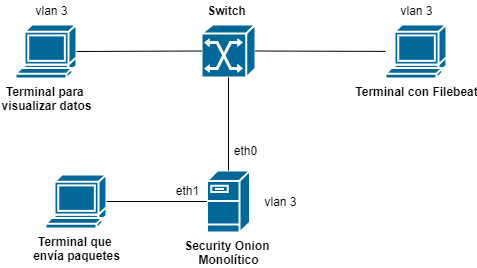
\includegraphics[width=0.8\textwidth]{./iteracion_1_imagenes/figura_33_a_topologia_de_prueba_1.png}
    \caption{Topología monolítica de laboratorio}
    \label{fig:figura_33_a}
    \end{figure}
    El tercer terminal (C) se conectó mediante un enlace a la interfaz “Eth1” del nodo Monolítico, enviando tráfico simulado mediante PCAPS conteniendo acciones ofensivas. Para lograr esta acción, en el terminal C se utilizó TCPreplay \cite{tcpreplay} para reenviar los PCAPS mencionados. Esta interfaz estaba configurada para monitorear el tráfico en busca de paquetes que pudieran contener una acción ofensiva. 
    Posteriormente se colocó en producción un nodo Monolítico. En la Figura \ref{fig:iter1_top_m_unc} se observa la topología de la organización incluyendo la conexión con este nodo. Este tiene su interfaz de monitoreo conectada al Switch 3, donde recibe el tráfico reenviado que se produce entre la Dependencia 1 y el mencionado switch.
    \begin{figure}[H]
    \centering
    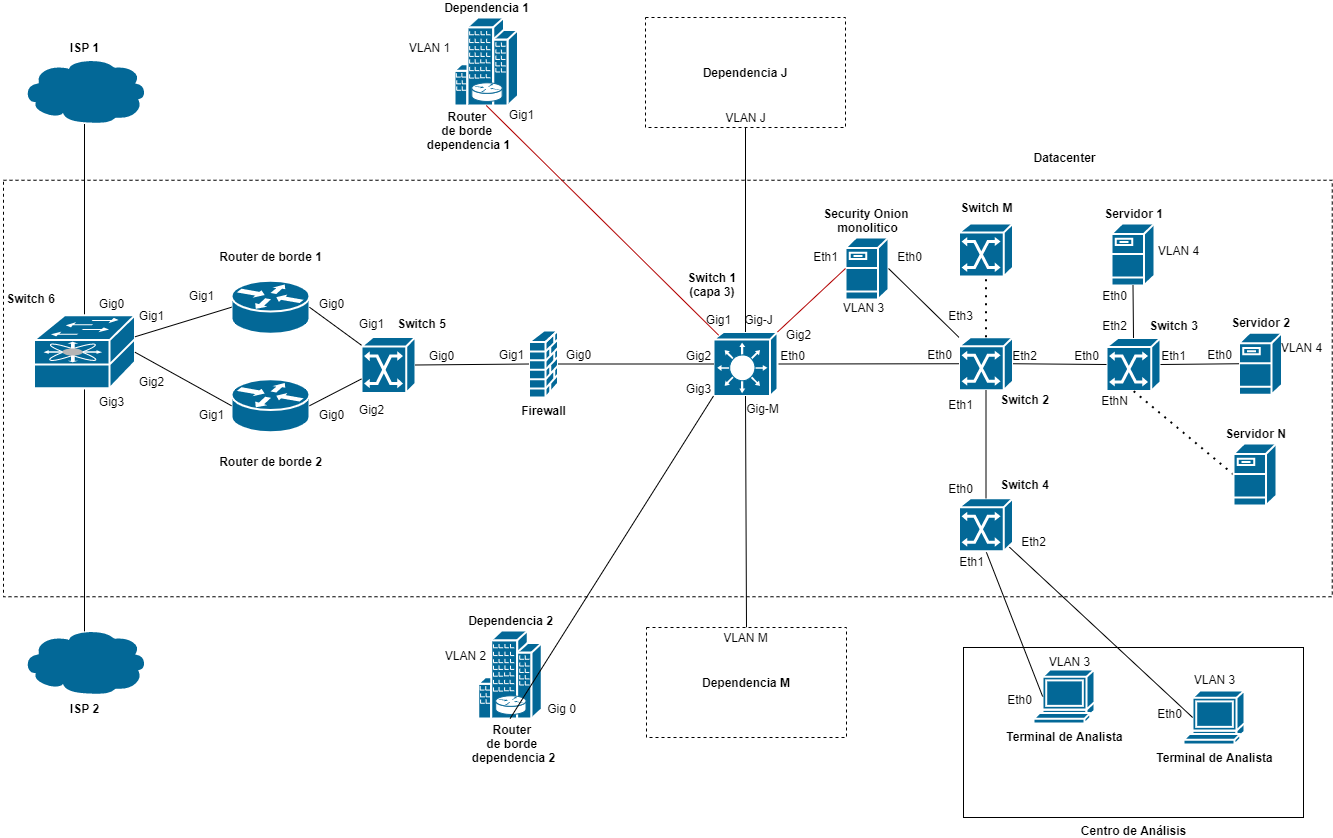
\includegraphics[width=1\textwidth]{./iteracion_1_imagenes/figura_topologia_m_unc.png}
    \caption{Despliegue de una topología monolítica de monitoreo}
    \label{fig:iter1_top_m_unc}
    \end{figure}
    \FloatBarrier
    Se realizaron pruebas de los requerimientos funcionales 1 y 3: se comprobó el funcionamiento de la recolección y almacenamiento de datos de incidentes de seguridad, al recibir y analizar tráfico proveniente de la Dependencia 1. \par
    %El nodo monolítico de Security Onion dispone de dos conexiones. La correspondiente al puerto eth0 es la que permite la administración del sistema y la consulta de sus datos, mientras que la interfaz eth1 es la destina a monitorear el tráfico de una red. En nuestro experimento con esta arquitectura, todo el tráfico fue simulado usando los PCAPS mencionados anteriormente. \par
    %En la Figura \ref{fig:iter1_top_m_unc} se observa la topología de la organización con un nodo Monolítico. Este tiene su interfaz de monitoreo conectada al Switch 3, donde recibe el tráfico reenviado que se produce entre la Dependencia 1 y el mencionado switch.
    
    \end{subsection}
    
    \begin{subsection}{Topología Distribuida de Monitoreo}
    \label{sec_topo_dist}
    Después de comprobar el funcionamiento de los principales componentes de Security Onion y obtener la experiencia descrita en la sección anterior, se procedió a considerar el despliegue de una topología distribuida. Este tipo de topología presenta considerables ventajas respecto de su alternativa monolítica, fundamentalmente en términos de rendimiento del hardware y flexibilidad de adaptación, como se mencionó en el Capítulo~\ref{tipos_de_arquitectura}.\par
    En primer lugar, se desplegó una versión simplificada para verificar el funcionamiento de los componentes de los dos nodos que la componen (nodos \textit{Forward} y \textit{Master}) y la comunicación entre ellos.
    \begin{figure}[H]
    \centering
    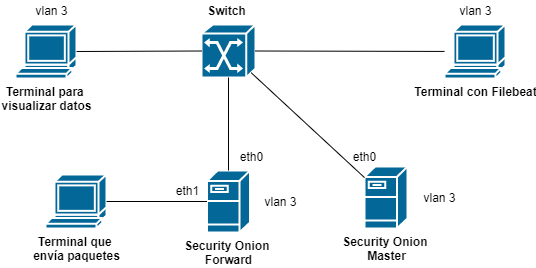
\includegraphics[width=1\textwidth]{./iteracion_1_imagenes/figura_33_b_topologia_de_prueba_2.png}
    \caption{Versión elemental de una topología distribuida}
    \label{fig:topologia_distribuida_1}
    \end{figure}
    Se observa en la Figura \ref{fig:topologia_distribuida_1} los componentes fundamentales de Security Onion para poder llevar a cabo esta topología: un nodo \textit{Forward} conectado a la interfaz a monitorear y un nodo \textit{Master} conectado al switch de la red interna. El nodo \textit{Master} y el \textit{Forward} se comunican mediante un enlace de administración (interfaz eth0 del nodo \textit{Forward}), que es el que está conectado al Switch. \par
    En este caso, como en el descrito en la sección anterior (\ref{subsec-topo-mono}), se utilizaron logs y tráficos de red obtenidos con anterioridad. El objetivo de esta experiencia fue comprobar el correcto funcionamiento de los dos nodos. Adicionalmente, con el motivo de probar la generación de notificaciones de alertas, se comprobó el funcionamiento de ElastAlert, que forma parte de los componentes del nodo \textit{Master}. \par
    La experiencia consistió en enviar logs desde la terminal con Filebeat hacia el nodo \textit{Master}, para que posteriormente fueran filtrados. Para esta tarea se empleó Logstash junto a un \textit{plugin} llamado Grok. Se buscó identificar campos de interés que estuvieran presentes en los \textit{logs} y se hallaron direcciones IP. Se crearon alertas en ElastAlert que se activaron al detectar estas IP y se enviaron mensajes por un servidor de correo electrónico (propio de la organización) y aplicaciones (Telegram y Slack). Los resultados de este experimento verificaron el RF4, que se trata en la iteración II (Capítulo \ref{iteracion2}). \par
    Si bien Security Onion incluye gran parte de los componentes de un SIEM, es necesario un sistema adicional que sea capaz de recolectar las alertas generadas en primera instancia por el nodo \textit{Master} y manipular esta información para lograr un manejo eficaz de los incidentes. Este sistema es TheHive. \par
    TheHive recibe las alertas generadas en el nodo \textit{Master} por ElastAlert y las introduce en un proceso de correlación de incidentes para proporcionar mayor información del mismo a los analistas del CSIRT. Cortex es un componente asociado a TheHive, que permite desarrollar y automatizar respuestas a incidentes. TheHive y Cortex, junto a los componentes del nodo \textit{Master} (Kibana y Squert) son los únicos componentes visibles con los que interactúan los analistas. \par
    
    Luego de la incorporación de TheHive, se volvió a repetir el experimento detallado anteriormente (Figura \ref{fig:topologia_distribuida_1}), esta vez con el objetivo de que TheHive recibiera las alertas generadas en el nodo \textit{Master} mediante ElastAlert. La topología del experimento se observa en la Figura \ref{fig:topologia_distribuida_2}.\par
    \begin{figure}[H]
    \centering         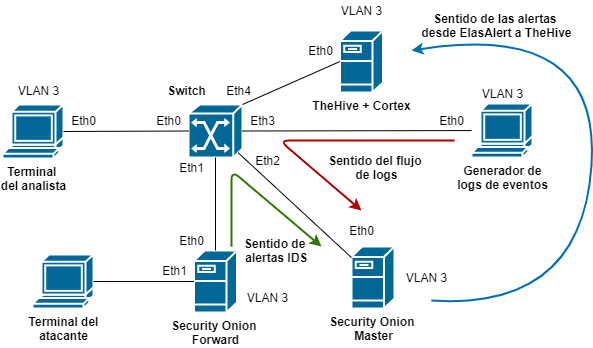
\includegraphics[width=1\textwidth]{./iteracion_1_imagenes/figura_33_e_topologia_de_prueba_3.png}
    \caption{Experiencia de laboratorio de la topología distribuida con todos sus componentes}
    \label{fig:topologia_distribuida_2}
    \end{figure}
    \FloatBarrier
    De esta manera, se completaron los componentes del SIEM al ofrecer un manejo centralizado de los datos de incidentes de seguridad de la información. Cuando el nodo \textit{Forward} identificó un  ataque, notificó al nodo \textit{Master} del mismo. En este último, ElastAlert generó alertas que fueron enviadas al servidor de TheHive, quien las presentó a los analistas junto a información contextual que intentó correlacionar con información presente en su base de datos.\par
    
    Finalmente, se procedió a desplegar la configuración final de la topología de la solución en este proyecto. Esta consistió en agregar un segundo nodo \textit{Forward} para monitorear el tráfico de una dependencia adicional, como se muestra en la Figura \ref{fig:iter1_top_d_unc}.
    \begin{figure}[H]
    \centering
    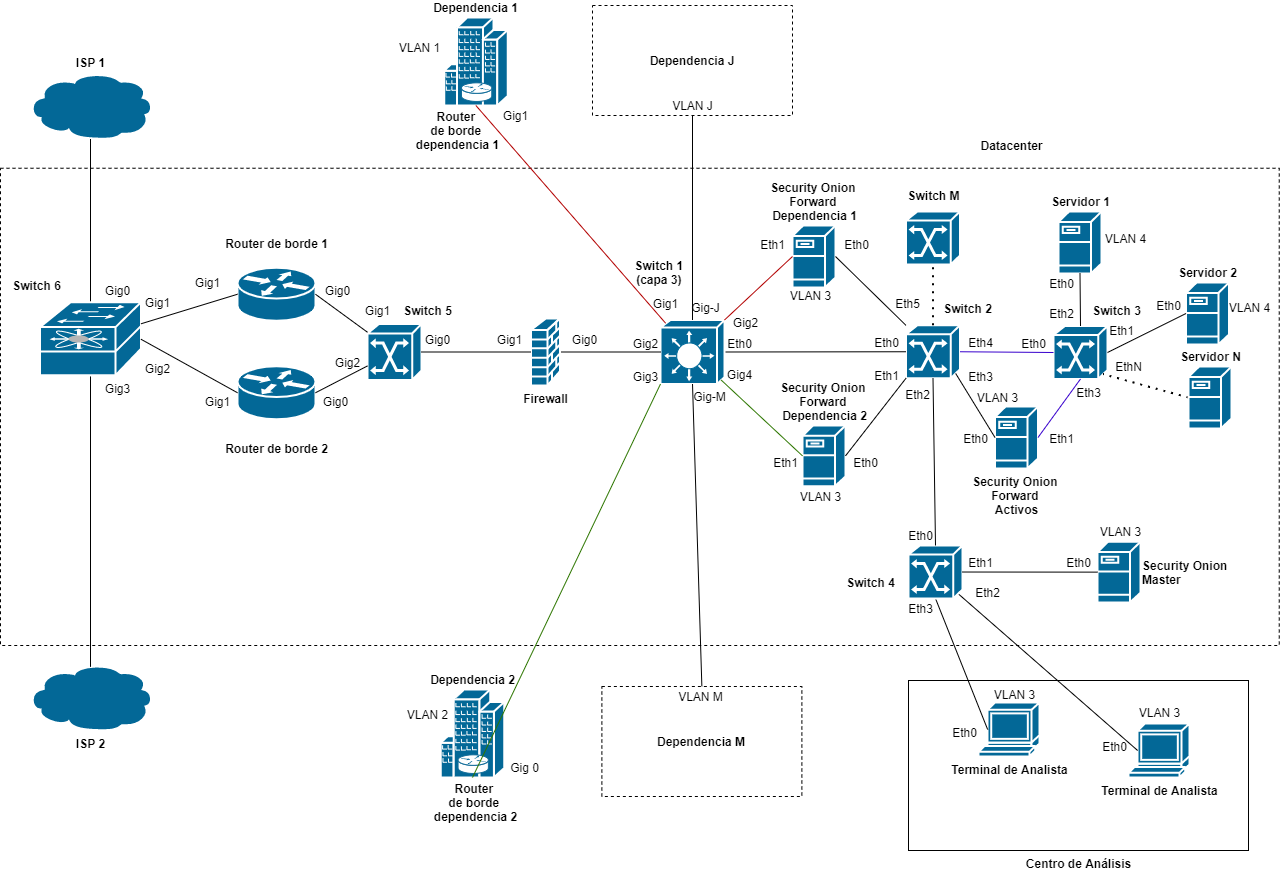
\includegraphics[width=1\textwidth]{./iteracion_1_imagenes/figura_topologia_d_unc.png}
    \caption{Despliegue de una topología distribuida de monitoreo}
    \label{fig:iter1_top_d_unc}
    \end{figure}
    La Figura \ref{fig:iter1_top_d_unc} muestra la topología de prueba donde se instaló Security Onion. Se observan los proveedores de conexión a internet (ISP) y la conexión con el \textit{router} de borde de la organización. Este último se conecta mediante un enlace \textit{gigabit} en el puerto Gig0 al puerto Gig4 del \textit{Switch} 1 (capa 3). \par
    El \textit{Switch} 1 es un dispositivo de red de capa 3, que conecta las dependencias entre sí y con el \textit{datacenter}. Las conexiones mencionadas se implementan físicamente sobre un enlace \textit{gigabit} de fibra óptica, pero virtualmente sobre redes tipo VLAN. De esta manera, por ejemplo, la Dependencia 1 está conectada físicamente por un enlace \textit{gigabit} a través de su puerto Gig1 de su \textit{router} de borde, con el puerto Gig5 del Switch 1 capa 3. Desde el punto de vista lógico, este enlace pertenece a la VLAN 1 de la organización. La situación descrita es análoga para el resto de las dependencias de la Universidad. \par
    Por otro lado, el \textit{Switch} 1 (en adelante SW 1), está conectado a los nodos \textit{Forward} 1 y 2 de Security Onion. Como resultado, es posible reenviar el tráfico entre SW1 y las dependencias 1 y 2 hacia los puertos Gig0 y Gig2 de SW1 que conectan SW1 con los nodos \textit{Forward} 1 y 2. \par
    SW1 está conectado con el \textit{Switch} 2 perteneciente al \textit{datacenter}, al cual se conectan a su vez los terminales de los analistas, los nodos \textit{Master} y \textit{Forward} (1 y 2) de Security Onion y TheHive. Esta topología permite desplegar una arquitectura distribuida de Security Onion, que fue la elegida para este proyecto.
    \end{subsection}
    \begin{section}{Verificación de RF1 y RF3}
    Luego de haber desplegado la topología distribuida que se observa de la Figura \ref{fig:iter1_ver_RF1_RF2}, se verificó el cumplimiento de los requerimientos RF1 y RF3. Para ello se llevó a cabo una acción ofensiva sobre un servidor ubicado en el \textit{datacenter}. Se seleccionó este servidor mediante un acuerdo con los responsables del área, para fines de evaluación de este proyecto. Este activo de la organización fue configurado a modo de prueba con un servidor web Apache versión 2.4.46, que contaba con una formulario web en PHP versión  7.2.21  y una base de datos MySQL versión 8.0.17.\par
    \begin{figure}[H]
    \centering
    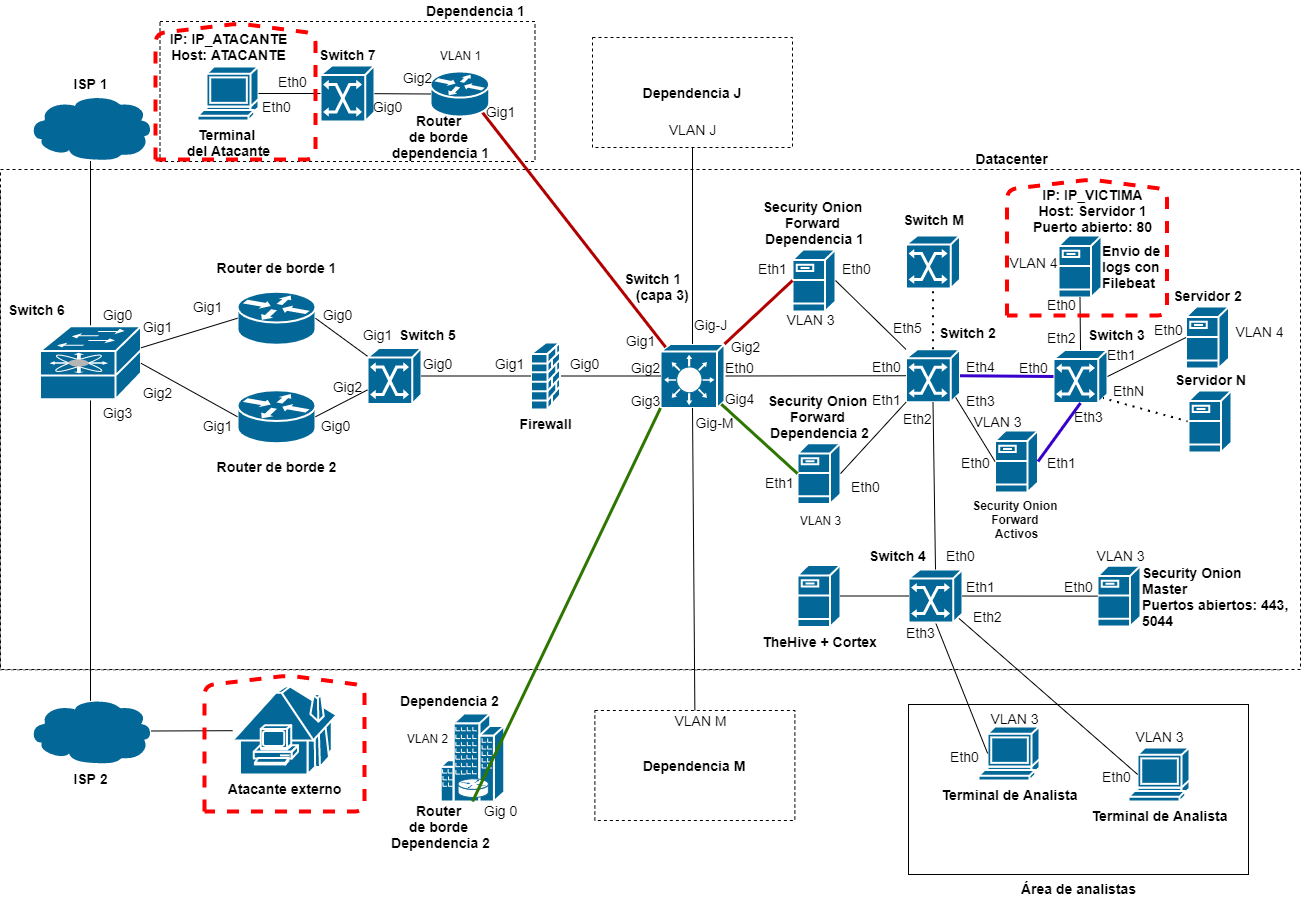
\includegraphics[width=1\textwidth]{./iteracion_1_imagenes/Topologia de despliegue descentralizada RF2, RF6 y RF4.png}
    \caption{Despliegue de una topología distribuida de monitoreo}
    \label{fig:iter1_ver_RF1_RF2}
    \end{figure}
    La acción ofensiva consistió en un ataque de reconocimiento que partió desde el \textit{host} ATACANTE ubicado dentro de la Dependencia 1 hacia la víctima llamada Servidor 1 que se encontraba dentro del \textit{datacenter}.
    Para realizar el ataque de reconocimiento se utilizaron rutinas de NMAP \cite{nmap} (versión 7.80) configuradas a tal fin: \textit{nmap -T4 -A -v IP\_VICTIMA} . Los parámetros utilizados fueron:
    \begin{itemize}
    \item -T4: para un escaneo intensivo (disminuye el tiempo de ejecución entre \textit{scripts})
    \item -A: habilita la detección del sistema operativo de la víctima y su versión, los \textit{scripts} de escaneo y \textit{traceroute}.
    \item -v: habilita el modo “verboso”.
    \item IP\_VICTIMA: es la dirección IP objetivo de este reconocimiento.
    \end{itemize}
    En la Figura \ref{fig:squert-nmap} se observa el panel de visualización de eventos de Squert.  En el recuadro rojo se encuentra la detección del ataque de reconocimiento realizado. El resto de la información que se aprecia en el panel principal corresponde a otros eventos que el sistema estaba detectando. Los eventos se agrupan según la categoría a la que pertenecen y un indicador de colores (barra vertical a la derecha del contador de eventos de cada fila) indica su prioridad de atención. %*Por defecto, Squert tiene su propia categoría de prioridades.
    Luego se observan la cantidad de eventos según su dirección, hora del último incidente ocurrido junto con su ID, una descripción de la firma del evento y el porcentaje de ocurrencia respecto al total de incidentes detectados.
    \begin{figure}[H]
    \centering
    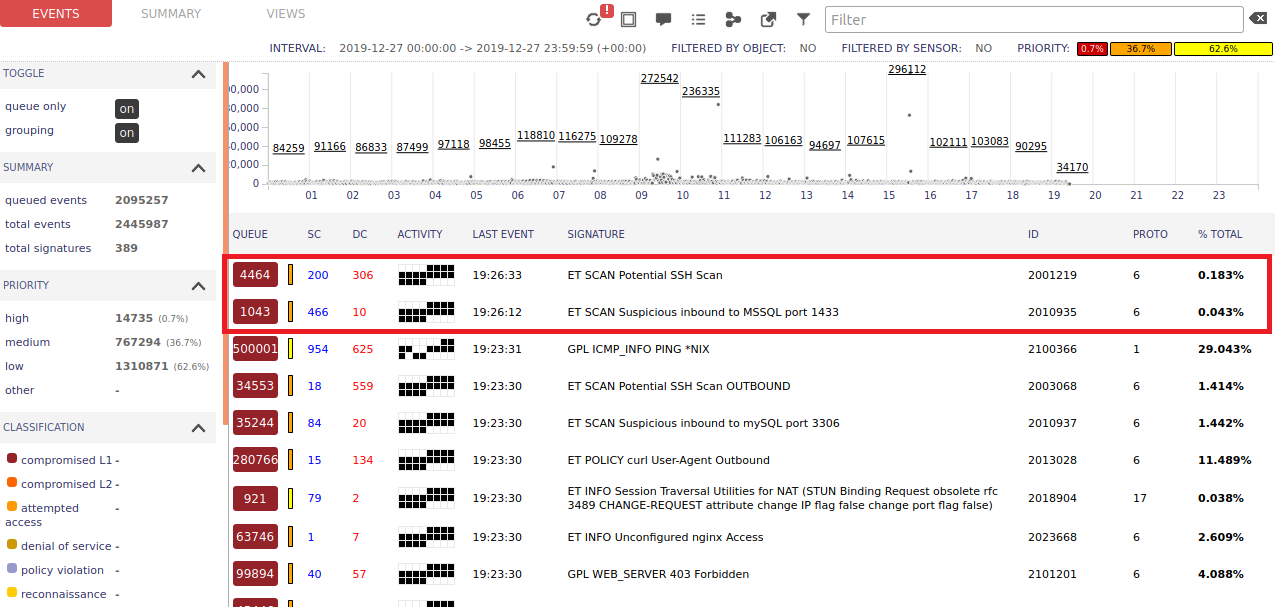
\includegraphics[width=1\textwidth]{./iteracion_1_imagenes/Squert_NMAP.png}
    \caption{Eventos visualizados en Squert}
    \label{fig:squert-nmap}
    \end{figure}
    \FloatBarrier
    En la Figura \ref{fig:thehive-nmap} se observa la visualización de la detección en TheHive. Si bien pueden ser similares, Squert se limita a mostrar los ataques similares agrupados en la misma categoría de incidente al que pertenecen, mientras que TheHive recibe las alertas de ElastAlert y presenta los eventos de manera individual. Esto permite a los analistas crear casos con cada incidente, correlacionarse con otros ataques, etc, lo que conduce a una gestión integral de eventos de seguridad.
    \begin{figure}[H]
    \centering
    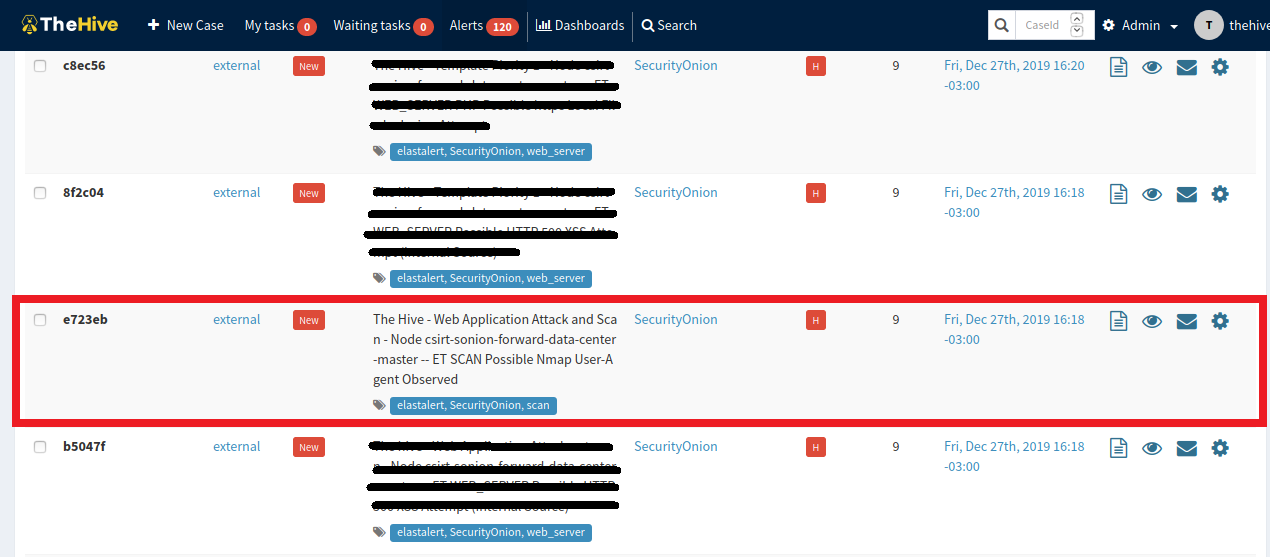
\includegraphics[width=1\textwidth]{./iteracion_1_imagenes/TheHive-NMAPEditado.png}
    \caption{Detección en TheHive del ataque de reconocimiento}
    \label{fig:thehive-nmap}
    \end{figure}
    \FloatBarrier
    Se verificó que las direcciones IP reportadas en el incidente por Squert y TheHive, coincidieran con las de la víctima y el atacante. Además mientras se estaba ejecutando el ataque, se hizo un seguimiento mediante Wireshark \cite{wireshark} filtrando las direcciones IP de origen y destino. Esto permitió corroborar el flujo de datos entre ambos.
    Los ataques fueron detectados por los nodos \textit{Forward} de la Dependencia 1 y \textit{Forward} Activos. \par
    Con esta prueba se verifica el cumplimiento de los requerimientos funcionales 1 y 3: “recolectar y almacenar datos de incidentes de seguridad en la infraestructura de la red corporativa ” y “visualizar las alertas en un tablero de mando”.\par
    \end{section} 
    
    
    \begin{section}{Colorario}
    En cuanto a la topología de la organización (Figura \ref{fig:iter1_top_unc}), podemos concluir que, la mejor opción para monitorear el tráfico entre las dependencias de la organización y el exterior fue conectar los nodos \textit{Forward} al \textit{Switch} 1 (el \textit{switch} troncal), para recibir el tráfico reenviado entre las dependencias y el mencionado \textit{switch}. Por otro lado, con el objetivo de lograr una defensa de punto final sobre activos de información específicos, fue necesario conectar un nodo \textit{Forward} al \textit{switch} (\textit{Switch} 2) al que se encuentran conectados estos activos. Estas conexiones se vieron reflejadas en la Figura \ref{fig:iter1_ver_RF1_RF2}. \par
    Se observó que la topología Monolítica fue ineficiente para el uso en entornos de producción, dado que la pila Elastic y los componentes de los sensores IDS de este nodo demandaron un uso intensivo de hardware. Si bien este tipo de topología fue útil a fines de probar el sistema o para monitorear enlaces de reducido tráfico y poco ancho de banda, resultó ineficaz en entornos más complejos. Esto se debió a los enormes requisitos de hardware necesarios para monitorear un enlace de 1 Gbps y considerando que el despliegue final requirió el monitoreo de múltiples enlaces con este ancho de banda, este tipo de topología fue incapaz de escalar utilizando el hardware disponible.\par
    Como consecuencia de la incapacidad de escalamiento horizontal descrita y siendo esta un requerimiento no funcional de este proyecto, se desplegó una topología distribuida de Security Onion. Los resultados del monitoreo fueron positivos, por lo cual se dio cumplimiento al RNF3, en simultáneo con la verificación de RF1 y RF3.\par
    

    \end{section}
    \chapter{\Large Iteración II: “Información contextual y envió de alertas de seguridad”}
\label{iteracion2}
    Partiendo de la topología definida en la Figura \ref{fig:iter1_top_m_unc} de Iteración I, se procedió a verificar los requerimientos de prioridad media. Para ello se siguió con la misma metodología de prueba, que consistió en un escaneo de puertos desde una terminal dentro de la Dependencia 1 a un activo ubicado dentro del datacenter llamado Servidor 1.
    \begin{section}{Verificación de RF2: Recolección de información contextual}
    Con el objetivo de recibir y procesar información contextual de los activos que se ven afectados durante un incidente, fue necesario configurar el servidor Master de Security Onion, con otros servicios que permitieran recibir información diferente de la provista por los sensores. Esta información refleja el estado de los servicios en un servidor, su conexión a la red, parámetros de uso de hardware como el nivel de ocupación de disco, temperatura, uso de la memoria RAM, los logs referidos al procesamiento de las peticiones que recibe un servidor, etc. \par
     Una anomalía en los datos de esta información no es suficiente por sí misma para confirmar un ataque, pero es útil para indicar que algo puede estar ocurriendo. En el caso de un ataque confirmado, estos datos representan evidencia forense y sirven para enriquecer modelos de amenazas complejas. \par
     Se decidió enviar la información contextual disponible mediante Filebeat. Este es un servicio que permite enviar información a Logstash desde múltiples directorios. El proceso comienza cuando el servicio lee línea por línea los archivos de entrada y envía los logs de la misma manera a Logstash. Este los recibe en su puerto 5044 por defecto, posteriormente puede filtrarlos para separar los campos de los logs o bien almacenarlos sin filtrar. \par
     Al principio se envió los logs del estado de las aplicaciones de un servidor disponible en la organización, mediante Filebeat, a Logstash y sin un procesamiento posterior. Esto generó que ElastAlert no pudiera realizar una correlación al no identificar información clave, como la que se encuentra en los campos de puertos y direcciones IP de origen y destino, estampas de tiempo, tipo de peticiones, etc.\par
     Posteriormente se utilizó el plugin Grok para filtrar los logs que estaba recibiendo Logstash antes de almacenarlos, de manera que la detección basada en correlaciones fue posible.\par
      Como se observa en la Figura \ref{fig:figura_iter2_ataque}, se realizó el envío de logs del Servidor 1 (que se encuentra conectado al Switch 3) mediante Filebeat al nodo Master que se encuentra conectado al Switch 4. Estos logs contenían información de un servidor web Apache, incluyendo consultas realizadas, métodos y otros metadatos de interés. Esta información resultó útil para identificar un ataque de fuerza bruta de estilo “inyección SQL”, que fue simulado utilizando herramientas como “sqlmap”, desarrolladas en Python 3.5. Este tipo de ataque consiste en introducir, de manera iterativa, comandos SQL en un formulario web con el objetivo de lograr recabar información de las bases de datos del Servidor 1 (víctima), modificar e incluso eliminar dicha base de datos. El comando utilizado en sqlmap fue: 
      \textit{python sqlmap.py -u "http://IP\_VICTIMA/login/index.php?id=101" --batch} donde los flags significan:
      \begin{itemize}
          \item \textit{-u}: parámetro para especificar una URL.
          \item \textit{“http://IP\_victima/path/al/formulario?etc”} es el campo que contiene la dirección de un formulario en la página web víctima.
          \item \textit{--batch}: es un switch que sirve para elegir la opción por defecto en paginas donde hay múltiples parámetros. La consecuencia de elegir la opción por defecto es que ahorra tiempo al evitar una elección del usuario.
      \end{itemize}
    \begin{figure}[H]
        \centering
        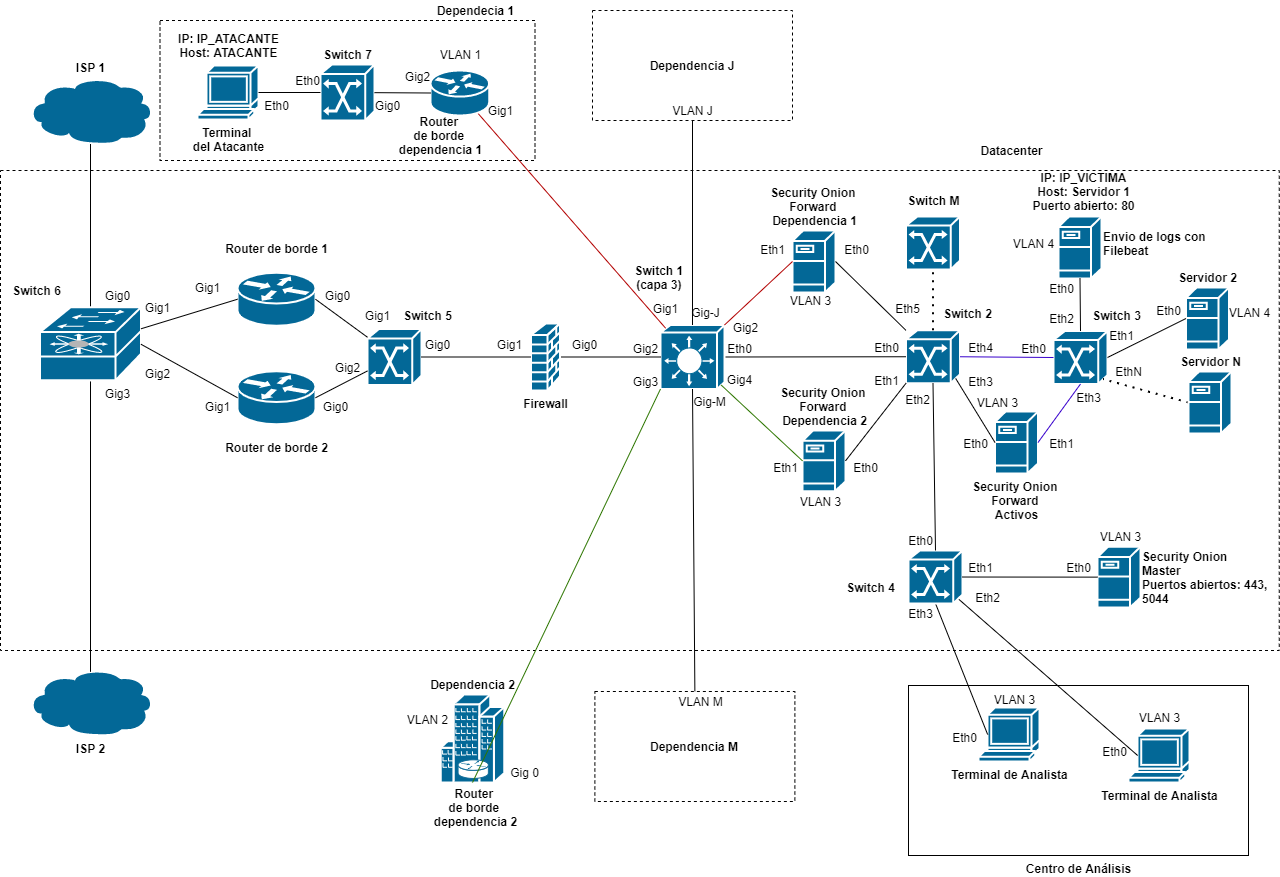
\includegraphics[width=1\textwidth]{./iteracion_2_imagenes/figura_iter2_ataque.png}
        \caption{Topología distribuida para la verificación de RF2, RF6 y RF4}
        \label{fig:figura_iter2_ataque}
    \end{figure}
    \FloatBarrier
    Como se mencionó anteriormente, en primer lugar los logs se almacenaron sin filtrar, lo que ocasionó que no fuese posible realizar algún tipo de correlación con los datos obtenidos. En la Figura \ref{fig:iter2_logs_crudos} se puede observar el almacenamiento de estos registros, con esto queda demostrado el cumplimiento del requerimiento funcional 2.
    \begin{figure}[H]
    \centering
        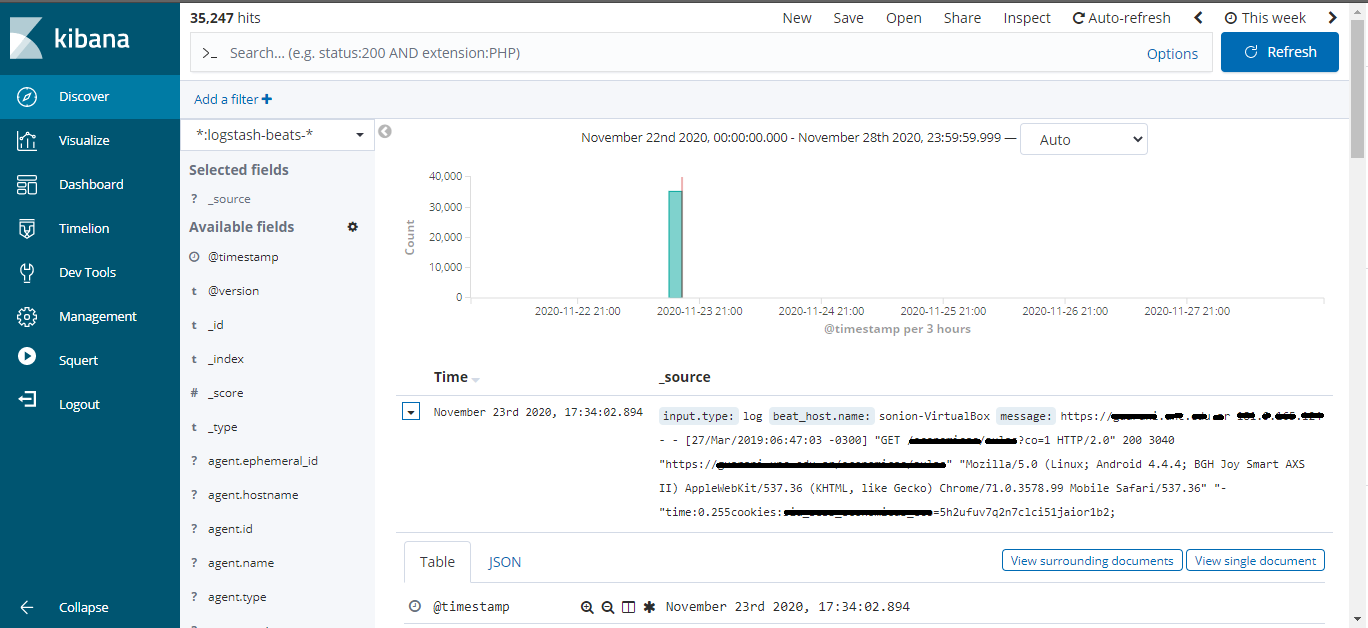
\includegraphics[width=1\textwidth]{./iteracion_2_imagenes/1_kibana_logs_1EDITADA.png}
        \caption{Almacenamiento de logs sin procesar}
        \label{fig:iter2_logs_crudos}
    \end{figure}
    Posteriormente se repitió la experiencia pero esta vez los logs que se recibían en Logstash eran procesados utilizando Grok. Este es un plugin de Logstash que permite filtrar datos sin ningún tipo de estructura y generar información estructurada capaz de ser consultada. \par
    En la Figura \ref{fig:figura_squert-sql} se pudo comprobar que el ataque de inyección SQL fue detectado en Squert.
    \begin{figure}[H]
    \centering
        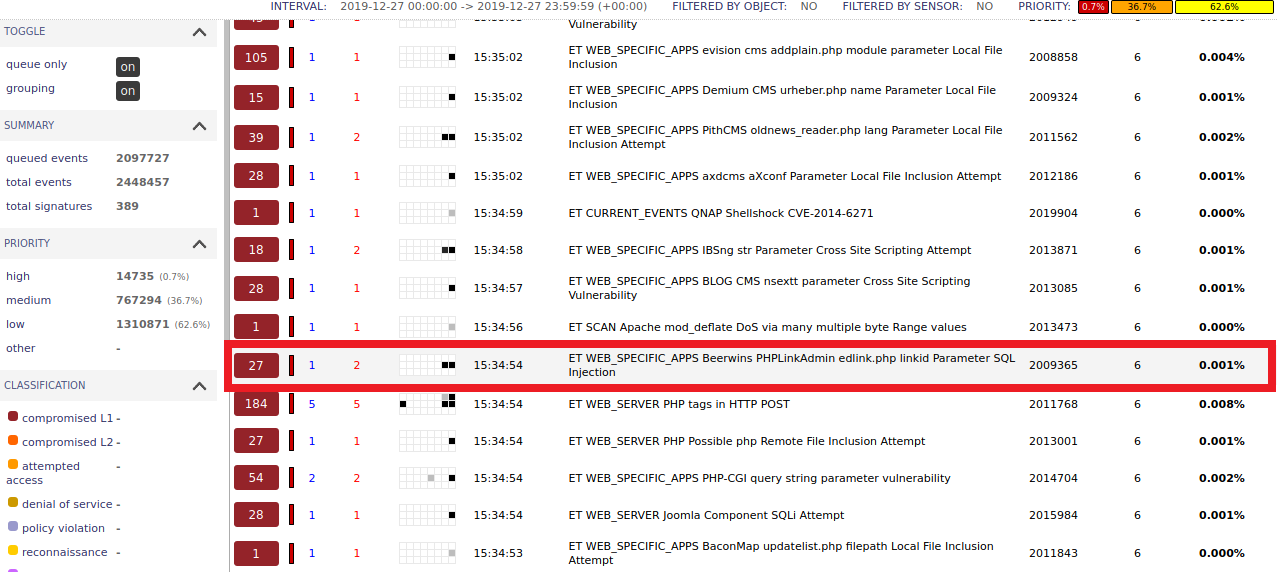
\includegraphics[width=0.7\textwidth]{./iteracion_2_imagenes/squert-sql-injection.png}
        \caption{Detección de un ataque de inyección SQL en el panel de Squert}
        \label{fig:figura_squert-sql}
    \end{figure}
    
    Los resultados en Kibana se ven en la Figura 6.3, donde se registraron las direcciones IP del Servidor 1 (víctima) y la del atacante. \par
    \begin{figure}[H]
    \centering
        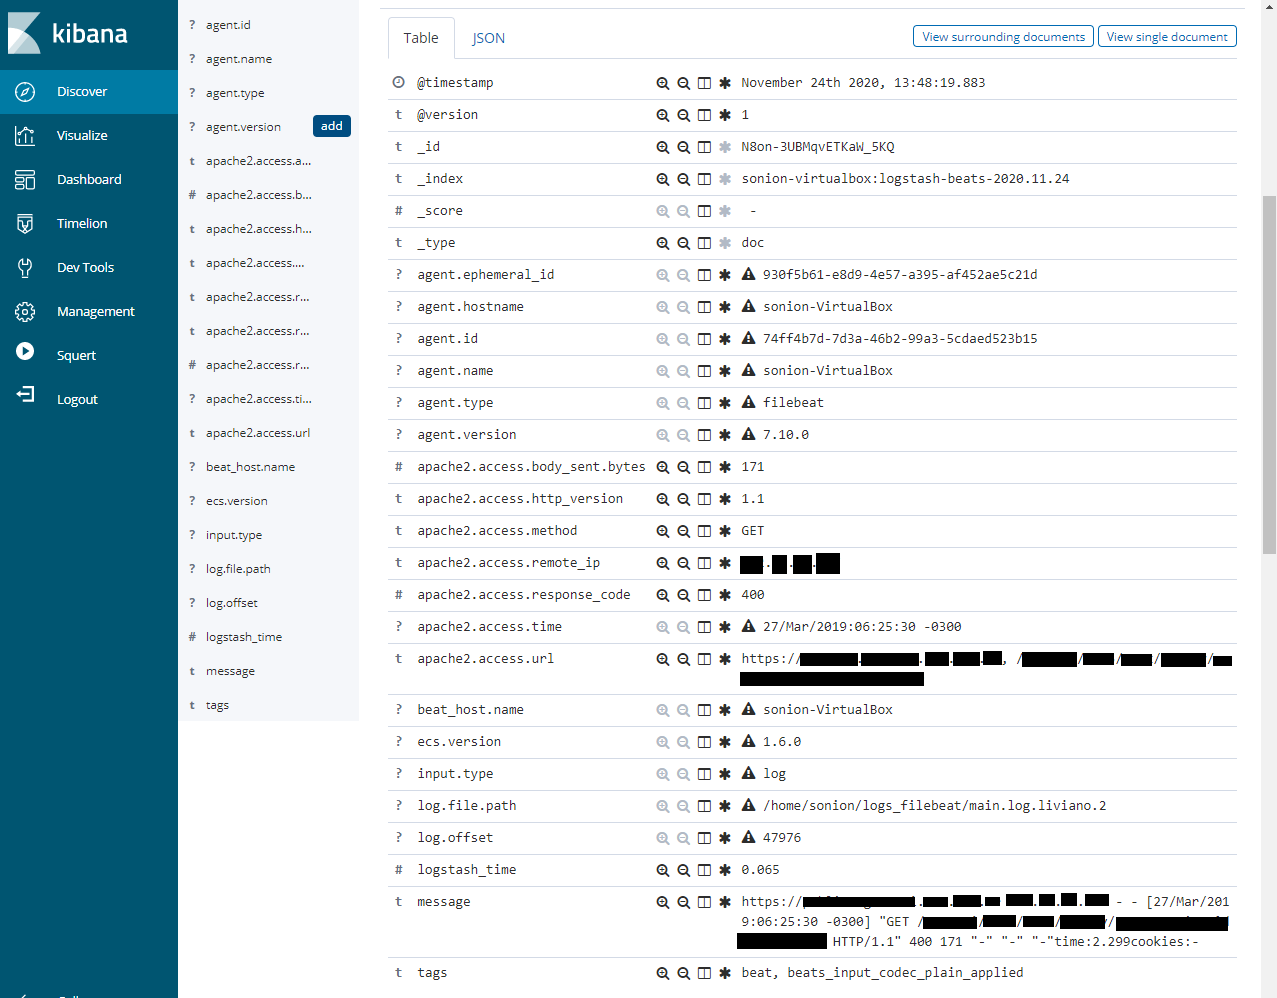
\includegraphics[width=1\textwidth]{./iteracion_2_imagenes/kibana_logs_parseados_2EDITADO.png}
        \caption{Almacenamiento de logs procesados por Logstash}
        \label{fig:iter2_logs_filtrados}
    \end{figure}
    
    Logstash posee varios filtros para todos los tipos de entradas que soporta. 
    Fue posible editar y administrar estos filtros utilizando archivos de configuración ubicados en la carpeta \textit{/etc/logstash/conf.d.available/}. Para este proyecto se eligió editar el filtro que procesa los datos provenientes de Filebeat, como se indicó anteriormente.\par
    Es importante mencionar que la información almacenada en Elasticsearch, es consultada constantemente por ElastAlert. Este último componente es el encargado de correlacionar los campos de los logs y enviar notificaciones.
    \end{section}
    \pagebreak
    
    \begin{section}{Verificación de RF6 y RF4: implementación de un sistema de correlación y envió de alertas de seguridad}
    El envío de alertas de seguridad y la notificación a los responsables de los activos que se ven afectados, fue realizado en este trabajo mediante ElastAlert. Este componente fue seleccionado ya que permite correlacionar la información presente en los campos de logs guardados en elasticsearch, así como enviar notificaciones cuando se produce la detección de incidentes. \par
    ElastAlert es un framework que detecta patrones en los datos consultados a Elasticsearch, como anomalías, picos, etc. Como se mencionó en la sección 4.5, basa su funcionamiento en dos componentes: reglas y alertas. \par
    Las alertas consisten en mensajes que permiten notificar a un usuario final o a otro sistema, sobre un evento de seguridad que ha ocurrido. Para esta prueba se decidió realizar nuevamente un escaneo de puertos desde el Atacante ubicado en la Dependencia 1 al Sevidor 1 víctima ubicado en el datacenter. Para esto se configuro a ElastAlert para que notifique por correo electrónico si este detectaba algún tipo de ataque de categoría “scan”.\par
     En la Figura \ref{fig:iter2_diagrama_envio_alertas} se observa un diagrama de secuencia del envío de una alerta.
    La secuencia comienza cuando los logs que llegan a Logstash son filtrados y enviados de forma estructurada (JSON) al puerto 9200 de Elastisearch. ElastAlert, por otro lado, realiza consultas periódicas a Elasticsearch. Cuando ElastAlert recibe una respuesta a su petición, procede a analizar los resultados en búsqueda de patrones que se puedan identificar en los logs recibidos. \par
    Independientemente de la coincidencia o no de algún patrón y la eventual notificación de alerta a los correspondientes responsables, ElastAlert vuelve a consultar a Elasticsearch por otros logs y procede a repetir el procedimiento descrito, mientras este activo como servicio.\par
    \begin{figure}[H]
    \centering
        \includegraphics[width=1\textwidth]{./iteracion_2_imagenes/2-diagrama-de-secuencia-envio-alerta.png}
        \caption{Diagrama de secuencia del envío de una alerta}
        \label{fig:iter2_diagrama_envio_alertas}
    \end{figure}
    Los patrones a buscar están definidos en las reglas habilitadas de ElastAlert y si se produce una coincidencia, se procede a enviar una notificación por los medios especificados en las reglas. Como se mencionó anteriormente, para esta prueba el medio elegido fue el correo electrónico de la organización. En la Figura \ref{fig:iter2_notificacion_alertas} se observa el correo electrónico recibido cuando se disparó una alerta sobre un ataque de reconocimiento. Con esto damos por verificado los RF4 y RF6, dado que para que la notificación haya sido enviada, previamente se tuvo que ejecutar una correlación, como se describió anteriormente.\par
    \begin{figure}[H]
    \centering
        \includegraphics[width=1\textwidth]{./iteracion_2_imagenes/notificacion_alertas_1EDITADO.png}
        \caption{Notificación recibida debido a una alerta por reconocimiento de puertos}
        \label{fig:iter2_notificacion_alertas}
    \end{figure}
    
    \end{section}
    \chapter{Iteración III: “Priorización de alertas”}
    En Security Onion y otros sistemas, el elemento descriptor que identifica y procesa a cada definición de incidente en particular es la regla. Las reglas comprenden una serie de campos que describen con precisión la naturaleza de un incidente dado y por lo tanto, existen tantas reglas como amenazas en circulación. \par
    Cuando un nuevo malware es descubierto por el equipo de algún CSIRT con la capacidad de investigación suficiente o reportado a un laboratorio apropiado para este fin, es posible realizar un estudio de sus características y una vez identificadas estas últimas, proceder a crear una regla y agregarla al repositorio correspondiente para que otros CSIRT actualicen sus IDS con esta nueva definición y así contar con un filtro (la regla) que permita detectar este malware. Las reglas tienen un conjunto de campos donde se detallan características del paquete y su contexto, tales como el puerto de origen y destino, protocolo empleado, dirección IP, etc y unos campos dedicados a la naturaleza del incidente (clasificación, mensaje, prioridad, etc). Algunos de estos campos son comunes a todas las reglas y permiten agruparlas para administrar eficientemente las alertas generadas cuando una regla coincide con la descripción de un incidente. Dado que estos campos también se pueden considerar observables, es posible utilizarlos por TheHive para gestionar incidentes y crear casos. \par

    \begin{section}{Verificación del requerimiento funcional 5: Definición de criterio para priorizar alertas.}
    Como se indicó anteriormente, la estructura de las reglas consisten en dos partes bien definidas: un encabezado (header) que es obligatorio  y un conjunto de campos opcionales. Dentro del header encontramos la acción (alerta, notificación, etc), el protocolo (tcp, udp), puertos de origen y destino, el sentido del evento (entrante o bidireccional) y las direcciones IP de origen y destino. \par
    La segunda parte de las reglas incluye dos tipos de campos: los que describen la naturaleza del evento y aquellos que contienen información del paquete de datos. Dentro del primer grupo encontramos aquellos tales como msg (descripción del evento), sid (id de la firma), classtype (clasificación de reglas o alertas), priority (prioridad de la firma y/o alerta), target (especifica de qué lado está el objetivo, es decir puerto de origen y puerto de destino), entre otros. El segundo grupo contiene datos extraídos que provienen desde de la capa de red hasta la de aplicación de la pila OSI. Se pueden mencionar a los campos “GeoIP” (localización geográfica de la IP), “Fragbits” (presencia del bit de fragmentación), “ACK” (presencia del campo ACK en paquete TCP), “itype” (número del tipo de mensaje ICMP), “http.method” (tipo de método HTTP usado), entre otros.
    \begin{figure}[H]
        \centering
        \includegraphics[width=0.7\textwidth]{./iteracion_3_imagenes/figura_41_estructura_regla.png}
        \caption{Estructura general de una regla}
        \label{fig:figura_41_estruc_regla}
    \end{figure}
    
    Como los campos están presentes en todas las reglas, es posible hacer uso de algunos de ellos para agrupar reglas que describen amenazas pertenecientes a un mismo grupo o categoría de malware, intentos de intrusión, reconocimiento, escalado de privilegios, etc y por lo tanto son útiles para gestionar los incidentes. \par
	Es posible configurar esta gestión a través de un archivo que relaciona campos como categorías de eventos con prioridades de la alerta generada. Este archivo llamado “classification.config” se encuentra bajo el directorio que almacena las reglas descargadas desde diversas fuentes; en particular relaciona los campos “classtype” con “priority”, de manera tal que cualquier regla cuyo campo classtype contenga a los descritos en este archivo, generará una alerta con prioridad definida también en este. De esta manera, es posible administrar un enorme número de reglas agrupadas en un reducido grupo de categorías y modificar el nivel de prioridad que tendrá en el sistema las alertas que generan. \par
	El objetivo de asignar distintos niveles de prioridad a las alertas generadas por los eventos que sucedan radica en la naturaleza de los eventos, su importancia y la gestión de la atención de los analistas del CSIRT. Esto se debe a las necesidades de optimizar el uso de los recursos técnicos y humanos del centro de respuesta a incidentes para cumplir de la manera más eficiente posible con los objetivos y políticas de la organización a la cual pertenece. De esta manera, la naturaleza de los incidentes determina su elegibilidad para una respuesta automatizada al tener en cuenta por un lado su estructura bien conocida y por el otro su alta tasa de repetición en un periodo determinado. En estos casos, sería inutil destinar valiosos recursos como la atención de un analista ya que conoce perfectamente la estructura del incidente y por lo tanto la respuesta apropiada o en aquellos casos en los que aún conocida su estructura, el incidente proviene en simultáneo de múltiples fuentes en muy poco tiempo, de manera que la capacidad humana de responder de a uno a la vez estaría tan sobrepasada que no sería efectiva. Estos son los casos de ataques de reconocimiento y los de denegación distribuida de servicio, entre otros. \par
	De aproximadamente cuarenta y siete (47) categorías de incidentes disponibles por defecto, consideramos para el máximo nivel de prioridad a siete clasificaciones dado su nivel de ocurrencia y nivel de impacto para la organización. 
    \begin{itemize}
        \item Web-application-attack: esta categoría engloba a un conjunto enorme de malware y ataques a nivel de capa de aplicación. Gusanos, ransomware, ataques de reconocimiento entre otras amenazas comparten esta categoría. Sobre el caso particular de los ataques de reconocimiento, se aplicaron filtros para separarlos de los demás ya mencionados. 
        \item Unsuccessful User: intentos repetidos de ganar acceso en ciertos activos e infraestructura de la organización.
        \item Attempted-dos: intentos de ataque de denegación de servicio y su variante distribuida
        \item Known client side exploit attempt: intento de ejecución de exploits en el lado del cliente.
        \item Exploit Kit Activity Detected: detección de actividad de un kit de exploits
        \item A suspicious filename was detected: detección de nombres de archivos sospechosos
        \item Network Trojan: detección de un virus troyano de red.
    \end{itemize}
    
    Para verificar el cumplimiento del requerimiento funcional 5, se procedió a editar el archivo  classification.config que se encuentra en el path /etc/nsm/rules/. En la Figura \ref{fig:squert-L2} se observa la detección de un incidente de reconocimiento en Squert. Este incidente pertenece a la categoría “attempted-recon” y en el archivo classification.config esta categoría tiene un nivel de prioridad 2, tal como se muestra en la figura (barra vertical naranja). Esto se puede observar con más detalle al analizar los campos de la alerta en Kibana, como se muestra en la Figura \ref{fig:Kibana-L2}. Se remarcó el campo “priority”, donde se vio que efectivamente el valor de la prioridad es 2.
    \begin{figure}[H]
        \centering
        \includegraphics[width=1\textwidth]{./iteracion_3_imagenes/squert_ataque_vnc_L2-EDITADO.png}
        \caption{Incidente de reconocimiento en Squert. Prioridad nivel 2}
        \label{fig:squert-L2}
    \end{figure}
    \begin{figure}[H]
        \centering
        \includegraphics[width=1\textwidth]{./iteracion_3_imagenes/kibana_ataques_L2_1EDITADO.png}
        \caption{Incidente de reconocimiento en Kibana. Prioridad nivel 2}
        \label{fig:Kibana-L2}
    \end{figure}
    \FloatBarrier
    Se modificó el archivo \textbf{classification.config} para elevar el nivel de prioridad de los eventos asociados a la categoría “\textit{attempted-recon}”, que pasó del nivel 2 al nivel 1. Posteriormente se reiniciaron los sensores mediante el comando “\textit{so-sensor-restart}” y se procedió a comprobar los resultados de la modificación. Se repitió el ataque de reconocimiento y se pudo observar en las Figuras \ref{fig:squert-L1} y \ref{fig:kibana-L1} que Squert detectaba el ataque con prioridad 1 (barra vertical roja) y en Kibana se observó que el campo “priority” contenía el valor 1. Con esto se da por cumplido el requerimiento funcional 5.
    
    \begin{figure}[H]
        \centering
        \includegraphics[width=1\textwidth]{./iteracion_3_imagenes/squert_ataque_vnc_L1-EDITADO.png}
        \caption{Incidente de reconocimiento en Squert. Nivel 1}
        \label{fig:squert-L1}
    \end{figure}
    \begin{figure}[H]
        \centering
        \includegraphics[width=1\textwidth]{./iteracion_3_imagenes/kibana_ataques_L2_2-EDITADO.png}
        \caption{Incidente de reconocimiento en Kibana. Nivel 1}
        \label{fig:kibana-L1}
    \end{figure}
    
    \end{section}
    
    \pagebreak
    \begin{section}{Requerimiento no funcional 4: Se requiere un despliegue automatizado de la solución}
    Para el despliegue automatizado de la solución se utilizó Ansible  2.8.4. Ansible es una herramienta de automatización de administración de servidores, utilizada en la organización donde se desplegó este proyecto. Esta herramienta permite ahorrar tiempo y esfuerzo al automatizar tareas repetitivas, disminuir errores y aumentar la productividad general cuando se trata del despliegue e instalación de infraestructura básica, como instalar sistemas operativos, realizar la configuración inicial de estos, etc. Es por esta razón que la organización requirió el desarrollo de scripts de instalación de nuestra solución en Ansible.\par
    En primer lugar, se desplegó una máquina virtual para probar el resultado de estos scripts. En esta máquina se instaló el sistema operativo Ubuntu Server 16.04 junto a los prerrequisitos para desplegar Ansible: Python en sus versiones 2.7 y 3.5, junto a su módulo pexpect (versión 4.7) y se configuraron las credenciales SSH entre esta máquina y el servidor desde el cual ordenamos el despliegue.\par
    Posteriormente se desarrolló un archivo de configuración de Security Onion para su despliegue. Si bien este archivo incluyó numerosos campos y variables, resaltan los correspondientes a la configuración de red, el tipo de rol (Master o Forward) y en base a esto las interfaces de monitoreo o administración, así como configuraciones de almacenamiento de logs, etc.\par
    Establecida la comunicación entre la máquina de destino y el servidor, se dio paso al inicio de la ejecución del script de Ansible. Para esto se ejecutó el comando “\textit{ansible-playbook -i hosts -l master so\_setup.yml --extra-var "target=sonionmaster"\hspace{1 mm} --ask-become-pass}”. En este caso, el comando especifica el despliegue de un nodo Master, sus flags y variables son las siguientes:
    \begin{itemize}
        \item \textit{ansible-playbook}: almacenan y ejecutan funciones de configuración, despliegue y orquestación de Ansible. Configura los pasos generales de un proceso de infraestructura IT y específica políticas para los sistemas remotos. 
        \item \textit{- i hosts}: flag que describe el inventario donde se encuentran los hosts. Esta varible \textit{host} es un archivo que describe las direcciones IP de las maquinas disponibles.
        \item \textit{- l}: opción utilizada junto al flag “\textit{-i}”, selecciona un subconjunto de hosts del inventario.
        \item \textit{--extra-var}: flag que configura variables adicionales como clave/valor o YAML/JSON. En nuestro ejemplo selecciona la opción \textit{sonionmaster} indica que se instaló un nodo Master de Security Onion.
        \item --ask-become-pass: flag que solicitó una contraseña de privilegio de usuario cuando fue necesario.
    \end{itemize}
    En el caso de la instalación de un nodo Forward, hubo que cambiar las opciones del  comando que se mencionó anteriormente. El resultado fue: “\textit{ansible-playbook -i hosts -l forward\_nodes so\_setup.yml --extra-var "target=sonionforward"\hspace{1 mm} --ask-become-pass}”. \par
    En el caso de la instalación de TheHive y Cortex, el proceso es análogo al descrito en el párrafo anterior.\par
    El comando para TheHive quedó de la siguiente manera: "\textit{ansible-playbook -i hosts -l thehive setup.yml --extra-var "target=thehiveuser"\hspace{1 mm}  --ask-become-pass}", mientras que en el caso de la instalación de Cortex, el comando resultante se muestra a continuación:
    "\textit{ansible-playbook -i hosts -l cortex setup.yml --extra-var "target=thehiveuser"\hspace{1 mm} --ask-become-pass}".\par
    Entre las acciones que realizó Ansible durante la ejecución de los scripts, se destacaron las de descargar e instalar los paquetes de Security Onion, para luego configurar el sistema operativo utilizando el archivo de configuración mencionado anteriormente. En el caso de la instalación de un nodo Forward, durante la configuración del sistema se debió ingresar la clave ssh para conectarse con el nodo Master.\par
    Finalmente se dio por satisfecho este requerimiento no funcional al comprobar que el sistema funcionaba correctamente.\par

    

    \end{section}
    \chapter{\Large Conclusión}
Haber desplegado una solución SIEM y en consecuencia, dotar al incipiente CSIRT de la Universidad Nacional de Córdoba con herramientas de monitoreo y gestión de eventos de seguridad de la información, permitió sumar nuevas capacidades de ciberseguridad a la Universidad. Estas consisten en poder monitorear el tráfico desde y hacia la universidad, incluyendo sus dependencias, infraestructura y activos de información.
 \par
Se logró desarrollar el sistema de monitoreo mediante el despliegue y configuración de Security Onion. A partir de este momento la Universidad pudo observar y analizar los eventos de seguridad de la información que estaban ocurriendo en su tráfico de datos.  \par
Fueron enfrentados varios desafíos, algunos de los cuales pudieron superarse con éxito y otros permanecen como tareas pendientes para posteriores trabajos. En cuanto a los problemas que pudieron ser resueltos se destacan la priorización de categorías de eventos, el aprendizaje y uso de las correlaciones que resuelve ElastAlert. Además fue posible aprender sobre la creación de filtros de eventos para disparar notificaciones específicas, identificar el comportamiento de determinados tipos de eventos, la administración inteligente del espacio en el disco y el desarrollo de scripts en TheHive. \par

Otro hecho a destacar es haber podido implementar este proyecto en un entorno complejo y con hardware de alto rendimiento, como es la infraestructura de redes de datos de la Universidad Nacional de Córdoba. Esto nos permitió experimentar y poner a prueba nuestro proyecto bajo condiciones reales y en un ambiente altamente demandante. Fue posible contemplar el desempeño de la solución y poner a punto el sistema. \par
Finalmente pudimos adquirir conocimientos y experiencia, en el área de la seguridad de redes de la información en particular y en ciberseguridad en general. Ensayamos el proceso, vimos sus efectos y consecuencias, de desplegar este tipo de soluciones a gran escala. Fue una gran experiencia haber explorado esta área profesional y haber adquirido aptitudes para desarrollar en el futuro. \par



    \chapter*{Futuros trabajos}
    
    % Bibliografía 
    \printbibliography
    \chapter*{\Large Anexos}
\addcontentsline{toc}{chapter}{Anexos}
    

\end{document}
